% template from https://fachschaft.tf.uni-freiburg.de/informationen/dokumentvorlagen
%
%
%
% documentclass options:
\documentclass[11pt,
  a4paper,
  parskip=half, % This is some extra vertical space between paragraphs, the suggestion is 2cm which is really ugly, so we use what koma script gives us
  % you can also set it to full for even more space. But there is a bad tex style decision: parskip also changes the spacing between listitems such as
  % enumerate and itemize. For this purpose we include the enumitem package and set itemsep=.5em, of course you can change this
  BCOR=10mm, % BCOR is binding correction
  ngerman,
  % if you'd rather have a one sided thesis, add `oneside' to the documentclass
  % onside,
  % ngerman is needed for hyphenation if the thesis contains parts written in German, switch order with english if you write mainly in English.
  % Remember to change order in the babel package (below) as well.
  % Last language is the preferred one.
  english]{scrbook}
\usepackage[ngerman,english]{babel} % If you write mainly in English change order to ngerman, english. Also change that in the documentclass options above.
% Include of titling must happen before \title etc.
% that's why it's not in setup.tex
\usepackage{titling}
\title{HybridCite: a Hybrid Embedding-IR Citation Recommendation System}
\author{Ashwath Sampath}

% Change to your first examiner
% The ~ enables non sentence spacing after a period
\newcommand{\firstexaminer}{Prof.~Dr.~Georg Lausen}
% Change to your second examiner, some undergraduate studies don't have a second examiner
% in this case just comment out the following line
\newcommand{\secondexaminer}{Dr.~Fang Wei-Kleiner}
% Change to your adivers
\newcommand{\advisers}{Dr.~Michael F{\"{a}}rber}

% include all packages and define commands in setup.tex

%------------------------------------------------------------------------------
%       package includes
%------------------------------------------------------------------------------
    % font encoding is set up for pdflatex, for other environments see
    % http://tex.stackexchange.com/questions/44694/fontenc-vs-inputenc
    \usepackage[T1]{fontenc}  % 8-bit fonts, improves handling of hyphenations
    \usepackage[utf8]{inputenc}  % remove if engine is switched to xelatex
    % provides `old' commands for table of contents. Eases the ability to switch
    % between book and scrbook
    \usepackage{scrhack}

    % better looking fonts
    \usepackage[tt=false, type1=true]{libertine}
    \usepackage{libertinust1math}


    % ------------------- layout, default -------------------
    % adjust the style of float's captions, separated from text to improve readabilty
    \usepackage[labelfont=bf, labelsep=colon, format=hang, textfont=singlespacing]{caption}
    % With format = hang your caption will look like this:
    % Figure 1: Lorem ipsum dolor sit amet,
    %           consectetuer adipiscing elit.
    %           Ut purus elit, vestibulum
    % If you instead want
    % Figure 1: Lorem ipsum dolor sit amet,
    % consectetuer adipiscing elit. Ut purus
    % elit, vestibulum
    % change to format=plain
    \usepackage{chngcntr}  % continuous numbering of figures/tables over chapters
    \counterwithout{equation}{chapter}
    \counterwithout{figure}{chapter}
    \counterwithout{table}{chapter}

    % Uncomment the following line if you switch from scrbook to book
    % and comment the setkomafont line
    %\usepackage{titlesec}  % remove "Chapter" from the chapter title
    %\titleformat{\chapter}[hang]{\bfseries\huge}{\thechapter}{2pc}{\huge}
    \setkomafont{chapter}{\normalfont\bfseries\huge}

    \usepackage{setspace}  % Line spacing
    \onehalfspacing
    % \doublespacing  % uncomment for double spacing, e.g. for annotations in correction

    % ------------------- functional, default-------------------
    \usepackage[dvipsnames]{xcolor}  % more colors
    \usepackage{array}  % custom format per column in table - needed on the title page
    \usepackage{graphicx}  % include graphics
    \usepackage{subfig}  % divide figure, e.g. 1(a), 1(b)...
    \usepackage{amsmath}  % |
    \usepackage{amsthm}   % | math, bmatrix etc
    \usepackage{amsfonts} % |
    \usepackage{calc}  % calculate within LaTeX
    \usepackage[unicode=true,bookmarks=true,bookmarksnumbered=true,
                bookmarksopen=true,bookmarksopenlevel=1,breaklinks=false,
                pdfborder={0 0 0},backref=false,colorlinks=false]{hyperref}
    \usepackage{etoolbox} % if-else commands


    %==========================================
    % You might not need the following packages, I only included them as they
    % are needed for the example floats
    % ------------------- functional, custom -------------------
    \usepackage{algorithm,algpseudocode}
    \usepackage{bm}  % bold greek variables (boldmath)
    % \usepackage{tikz}
    % \usetikzlibrary{positioning}  % use: above left of, etc

    % Improves general appearance of the text
    \usepackage[protrusion=true,expansion=true, kerning]{microtype}
    % \usepackage[protrusion=true]{microtype} % in case a switch to xelatex is
    %                                           necessary
    \usepackage{enumitem}

    % usually you don't need this, just for demonstration of a longer caption
    % \usepackage{lipsum}

    % toprule/midrule style tables
    \usepackage{booktabs}
    % make footnotes in tables work
    \usepackage{footnote}
    \makesavenoteenv{tabular}
    \makesavenoteenv{table}
    % enable listings
    \usepackage{listings}
    \lstset{literate=
      {Ş}{{\c{S}}}1 {ğ}{{\v{g}}}1,
      frame=top,frame=bottom,
      breaklines=true,
      basicstyle=\linespread{1}\footnotesize\ttfamily,
      escapeinside={(*}{*)},
      title=\lstname
    }
    % enable appenix
    \usepackage[toc,page]{appendix}
    \noappendicestocpagenum
    % long table for appendix
    \usepackage{longtable}
    % nice hyphens for citation lists
    \usepackage{cite}

%------------------------------------------------------------------------------
%       (re)new commands / settings
%------------------------------------------------------------------------------
    % ----------------- referencing ----------------
    \newcommand{\secref}[1]{Section~\ref{#1}}
    \newcommand{\chapref}[1]{Chapter~\ref{#1}}
    \renewcommand{\eqref}[1]{Equation~(\ref{#1})}
    \newcommand{\figref}[1]{Figure~\ref{#1}}
    \newcommand{\tabref}[1]{Table~\ref{#1}}

    % ------------------- colors -------------------
    \definecolor{darkgreen}{rgb}{0.0, 0.5, 0.0}
    % Colors of the Albert Ludwigs University as in
    % https://www.zuv.uni-freiburg.de/service/cd/cd-manual/farbwelt
    \definecolor{UniBlue}{RGB}{0, 74, 153}
    \definecolor{UniRed}{RGB}{193, 0, 42}
    \definecolor{UniGrey}{RGB}{154, 155, 156}


    % ------------------- layout -------------------
    % prevents floating objects from being placed ahead of their section
    \let\mySection\section\renewcommand{\section}{\suppressfloats[t]\mySection}
    \let\mySubSection\subsection\renewcommand{\subsection}{\suppressfloats[t]\mySubSection}


    % ------------------- marker commands -------------------
    % ToDo command
    \newcommand{\todo}[1]{\textbf{\textcolor{red}{(TODO: #1)}}}
    \newcommand{\extend}[1]{\textbf{\textcolor{darkgreen}{(EXTEND: #1)}}}
    % Lighter color to note down quick drafts
    \newcommand{\draft}[1]{\textbf{\textcolor{NavyBlue}{(DRAFT: #1)}}}


    % ------------------- math formatting commands -------------------
    % define vectors to be bold instead of using an arrow
    \renewcommand{\vec}[1]{\mathbf{#1}}
    \newcommand{\mat}[1]{\mathbf{#1}}
    % tag equation with name
    \newcommand{\eqname}[1]{\tag*{#1}}


    % ------------------- pdf settings -------------------
    % ADAPT THIS
    \hypersetup{pdftitle={\thetitle},
                pdfauthor={\theauthor},
                pdfsubject={Master's thesis at the Albert Ludwig University of Freiburg},
                pdfkeywords={citation recommendation, recommender system, data set, master thesis},
                pdfpagelayout=OneColumn, pdfnewwindow=true, pdfstartview=XYZ, plainpages=false}


    %==========================================
    % You might not need the following commands, I only included them as they
    % are needed for the example floats

    % ------------------- Tikz styles -------------------
    % \tikzset{>=latex}  % arrow style

    % ------------------- algorithm ---------------------
    % Command to align comments in algorithm
    \newcommand{\alignedComment}[1]{\Comment{\parbox[t]{.35\linewidth}{#1}}}
    % define a foreach command in algorithms
    \algnewcommand\algorithmicforeach{\textbf{foreach}}
    \algdef{S}[FOR]{ForEach}[1]{\algorithmicforeach\ #1\ \algorithmicdo}

    % line spacing should be 1.5
    \renewcommand{\baselinestretch}{1.5}

    % set distance between items in a list, for more details see the
    % enumitem package: https://www.ctan.org/pkg/enumitem
    \setlist{topsep=0pt,itemsep=0ex,partopsep=1ex,parsep=0ex}


\begin{document}
    \pagestyle{empty} % no header and no page number
    % disable hyper links to remove warning "destination with same identifier"
    % this means within this section nothing can be referenced with a hyperlink
    \hypersetup{pageanchor=false}

    % enable/disable, depending on your chosen language
    
\begin{titlepage}
\begin{center}

\newcommand{\HorizontalLine}{\rule{\linewidth}{0.3mm}}

{\Large Master's Thesis}\\[1.3cm]


% _____________________________________________________________________________
\HorizontalLine \\[0.4cm]
% Write your title in a fancy way like this if you want to customize it, otherwise simply let tex do it for you
% \begin{spacing}{3}
%     {\huge \bfseries The Long, Long } \\
%     {\huge \bfseries Long Long} \\
%     {\huge \bfseries Title}\\
% \end{spacing}
{ \huge \bfseries \thetitle }
\HorizontalLine \\[1.5cm]
% _____________________________________________________________________________


{\Huge \theauthor} \\[2cm]


\begin{tabular}[hc]{>{\huge}l >{\huge}l}
  Examiners: & \firstexaminer \\[0.3cm]
             & \secondexaminer \\[1.2cm]
\end{tabular}
\vfill  % move the following text to the bottom

\Large {
    Albert-Ludwigs-University Freiburg\\
    Faculty of Engineering\\
    Department of Computer Science\\
    Chair of Databases and Information Systems\\[1cm]

    June 26\textsuperscript{th}, 2019\\
}
\end{center}
\end{titlepage}

\thispagestyle{empty}
% title page back
\ \vfill \ \\  % at least one space required before vfill
\
\textbf{Writing Period}            \smallskip{} \\
15.\,10.\,2018 -- 26.\,06.\,2019   \bigskip{} \\
\
\textbf{First Examiner}                  \smallskip{} \\
\firstexaminer                     \bigskip{} \\
\
% If there is a second examiner include it
\ifdef{\secondexaminer}
	{
	% Include
	\textbf{Second Examiner}       \smallskip{} \\
	\secondexaminer                \bigskip{} \\
	\
	}
	{
	% No second examiner, ignore
	}
\textbf{Supervisor}                  \smallskip{} \\
\advisers

    %\begin{titlepage}
\begin{center}

\newcommand{\HorizontalLine}{\rule{\linewidth}{0.3mm}}

{\Large Master-Thesis}\\[1.3cm]


% _____________________________________________________________________________
\HorizontalLine \\[0.4cm]
% Write yourtitle in a fancy way like this if you want to customize it, otherwise simply let tex do it for you
% \begin{spacing}{3}
%     {\huge \bfseries Der Lange, Lange } \\
%     {\huge \bfseries Lange Lange} \\
%     {\huge \bfseries Titel}\\
% \end{spacing}
{ \huge \bfseries \thetitle }
\HorizontalLine \\[1.5cm]
% _____________________________________________________________________________


{\Huge \theauthor} \\[2cm]


\begin{tabular}[hc]{>{\huge}l >{\huge}l}
  Gutachter: & \firstexaminer \\[0.3cm]
             & \secondexaminer \\[1.2cm]
\end{tabular}
\vfill  % move the following text to the bottom

\Large {
    Albert-Ludwigs-Universität Freiburg\\
    Technische Fakultät\\
    Institut für Informatik\\
    Lehrstuhl für Datenbanken und Informationssysteme\\[1cm]

    26 June 2019
    \\
}
\end{center}
\end{titlepage}

\thispagestyle{empty}
% title page back
\ \vfill \ \\  % at least one space required before vfill
\
\textbf{Bearbeitungszeit}            \smallskip{} \\
15.\,10.\,2018 -- 26.\,06.\,2019   \bigskip{} \\
\
\textbf{Erstgutachter}                  \smallskip{} \\
\firstexaminer                      \bigskip{} \\
\
% If there is a second examiner include it
\ifdef{\secondexaminer}
	{
	% Include
	\textbf{Zweitgutachter}        \smallskip{} \\
	\secondexaminer                \bigskip{} \\
	\
	}
	{
	% No second examiner, ignore
	}
\textbf{Betreuer}                  \smallskip{} \\
\advisers


    \pagestyle{plain} % remove chapter name from top, page number at the bottom
    % use \pagestyle{headings} for having the chapter on top of the pages
    % if you want a more fancy header use \usepackage[automark,headsepline]{scrlayer-scrpage}
    % and read about it in the KOMA script documentation, https://www.ctan.org/pkg/koma-script
    \frontmatter  % roman page numbers
    % official declaration from the examination office; to be sure double
% check the wording on their website
% (https://www.tf.uni-freiburg.de/studies/exams/thesis/thesis_formatting.html#erklaerung)

\chapter*{Declaration}

I hereby declare, that I am the sole author and composer of my thesis and that no other sources or learning aids, other than those listed, have been used. Furthermore, I declare that I have acknowledged the work of others by providing detailed references of said work.  \newline
I hereby also declare, that my Thesis has not been prepared for another examination
or assignment, either wholly or excerpts thereof.
\\[3\normalbaselineskip]
\begin{tabular}{p{\textwidth/2} l}
  \rule{\textwidth/3}{0.4pt}   &   \rule{\textwidth/3}{0.4pt} \\
  Place, Date                  &   Signature
\end{tabular}

    \chapter*{Abstract}
The rate of publication of scientific papers has grown exponentially in recent years. As a result, it has become increasingly difficult for a researcher to find papers related to their research topic that are 'cite-worthy'. As in search engines, e-commerce and other fields which have had to deal with the information explosion problem, recommender systems have come to the rescue. Citation recommendation systems, which have been actively researched in the last few years, recommend citations for either a complete paper or a small portion of text called a \textit{citation context}. The process of recommending citations for citation contexts is called local citation recommendation, and is the focus of this thesis.
The Microsoft Academic Graph (MAG) data set, which has not been used in the local citation recommendation setting so far, is used in this thesis to train models using several algorithms based on embeddings, topic modelling and information retrieval techniques. The MAG data set is a rich data set containing both citation data and paper metadata, making it ideal for this task. 
The models created using the aforementioned algorithms are evaluated extensively offline using the MAG and other data sets created expressly for that purpose. Another data set created from the MAG helps to prove that citation contexts describe the cited paper more than the citing paper.
The best-performing algorithms are combined into a hybrid algorithm, which is evaluated offline as well as online by conducting a user study. The results show that a hybrid model containing embedding and information retrieval-based components outperforms its individual components by a large margin, and outperforms the other algorithms used in the thesis as well. This hybrid model is used to create a running recommender system, which is made available to the public.

\chapter*{Zusammenfassung}
Die Veröffentlichungsrate von wissenschaftlichen Arbeiten ist in den letzten Jahren exponentiell gestiegen. Infolgedessen ist es für einen Forscher immer schwieriger geworden, zu seinem Forschungsthema passende Arbeiten zu finden, die „zitierwürdig“ sind. Wie in Suchmaschinen, E-Commerce und anderen Bereichen, die sich mit dem Problem der Informationsexplosion befassen mussten, sind Empfehlungssysteme zur Rettung gekommen. Zitierempfehlungssysteme, die in den letzten Jahren aktiv erforscht wurden, empfehlen Zitate für eine vollständige Arbeit oder einen kleinen Teil des Textes, der als \textit{Zitierkontext} bezeichnet wird. Der Prozess der Empfehlung von Zitaten für Zitierkontexte wird als lokale Zitierempfehlung bezeichnet und steht im Mittelpunkt dieser Arbeit.
Der Microsoft Academic Graph (MAG)-Datensatz, der bisher nicht für lokale Zitierempfehlung verwendet wurde, wird in der Arbeit zum Trainieren von Modellen mit verschiedenen Algorithmen verwendet, die auf Einbettungen, Themenmodellierung und Information Retrieval-Techniken basieren. Der MAG-Datensatz ist ein umfangreicher Datensatz, der sowohl Zitierdaten als auch Papiermetadaten enthält und sich ideal für diese Aufgabe eignet.
Die mit den genannten Algorithmen erstellten Modelle werden weitgehend offline mit dem MAG und anderen eigens dafür erstellten Datensätzen ausgewertet. Ein anderer Datensatz, der aus dem MAG erstellt wurde, hilft zu beweisen, dass Zitierkontexte das zitierte Papier mehr beschreiben als das zitierte Papier.
Die leistungsstärksten Algorithmen werden zu einem Hybridalgorithmus kombiniert, der durch eine Anwenderstudie sowohl offline als auch online ausgewertet wird. Die Ergebnisse zeigen, dass ein Hybridmodell, das eingebettete und auf dem Abruf von Informationen basierende Komponenten enthält, seine einzelnen Komponenten um ein Vielfaches übertrifft und auch die anderen in der Arbeit verwendeten Algorithmen übertrifft. Mit diesem Hybridmodell wird ein laufendes Empfehlungssystem erstellt, das der Öffentlichkeit zugänglich gemacht wird.
    \tableofcontents
    %\listoffigures
    %\listoftables
    \hypersetup{pageanchor=true}  % re-enable hyperlinking

    \mainmatter  % Arabic page numbers
    \chapter{Introduction}\label{chap:introduction}
\section{Motivation}
Citations are the lifeblood of academic research papers. They provide a measure of trustworthiness, and can be used to either back up the authors’ claims using earlier research, to improve upon existing methods, or even to criticise research done previously. Moreover, citations are a way for researchers to give their readers an opportunity to compare and contrast the research in their papers with the research of other authors. 

%TODO This doesn't lead into the next para properly
The number of new scientific publications has been on a steep upward curve in recent years (detailed statistics in \cite{stm2008}). While this has made research more accessible than at any point in history, it has also made the researcher's task of finding a suitable paper to refer to and cite more difficult than ever before. All this has led to an increased amount of research being done on citation recommendation -- the process of finding and recommending prior work based on a passage of text.
This passage of text, usually called the \textit{citation context}, can be of different lengths: from a phrase or sentence, to a few sentences, to a paragraph or two.

\section{Problem setting}
If recommendations are made for the entire paper, the recommendations are \textit{global} and coarse-grained. Some of the earliest papers on citation recommendation covered global citation recommendation (~\cite{McNeeACGLRKR02}, ~\cite{StrohmanCJ07} and \cite{NallapatiAXC08}), but it has also been researched in multiple papers recently, for example, in ~\cite{Bhagavatula2018}, ~\cite{YangZCDMGD18} and \cite{CaiHY18}.

In this thesis, however, we will focus more on \textit{local citation recommendation}, in which a relatively small citation context (1-3 sentences or 50-100 words, for instance) is used. This type of fine-grained recommendation, sometimes also referred to as \textit{context-aware citation recommendation} in contemporary research papers, was first explored in \cite{He2010} and \cite{He2011}. 

This thesis will use the Microsoft Academic Graph (MAG) data set \cite{Sinha2015}, which has not been used in any of the papers in the area of local citation recommendation. Two papers have used the old version of Microsoft Academic in 2015 (\cite{ChakrabortyMNN15, Gao15}). However, both these papers do not implement local citation recommendation. 

Another important point to mention here is that there are 'personalised' approaches such as \cite{Ebesu2017} and \cite{YangZCDMGD18} which use the author and venue metadata as input for their algorithms. These obtain better scores on the evaluation metrics. However, as explained in \cite{Bhagavatula2018}, this is due to the fact that prediction of obvious citations (citations by the same author, for example) result in better scores on the metrics. This thesis will not consider such personalised approaches.

Now that we have seen what problem this thesis attempts to solve, it's time to briefly outline the methods that will be used to solve this problem in the next section.
\section{Method}
In conjunction with the data set prepared from MAG (which will be made available to the public), we will adapt different approaches to the problem of citation recommendation -- \textit{embedding approaches}, topic modelling approaches and standard Information Retrieval approaches. These will be discussed in detail in the following chapters.

A number of data sets based on the MAG are prepared, with restrictions made on the language and discipline (English and Computer Science respectively). The other data sets used are the Arxiv data set~\footnote{https://arxiv.org/}, the ACL-ARC data set~\cite{BirdDDGJKLPRT08} and a data set created from the open Unpaywall database~\footnote{https://unpaywall.org}. All of these are mapped to the MAG, combined with it, and made publicly available as well. 

Two existing deep-learning based embedding methods are adapted: one based on the Hyperdoc2vec paper by Han et al \cite{ShiSZZH18} and the other based on the Paper2vec paper by Ganguly et al \cite{GangulyP17}. In addition, a BM25-based recommender is prepared, along with baselines based on Latent Dirichlet Allocation (LDA) \cite{BleiNJ03} and Paragraph Vectors \cite{LeM14}. The best-performing methods are finally combined in a weighted hybrid recommendation system, which improves scores on the metrics markedly. 

The evaluation consists of two phases, an offline and an online one. The metrics used are ones which are commonly used in recommender systems research: MAP, Recall, MRR and NDCG. These metrics are calculated at different values of k for all the data sets.
While the offline evaluation phase provides one measure of how well the recommender system works, it is useful to have an online phase to manually judge the quality of recommendation results. Even if the list of recommendations does not contain the papers present in the ground truth, it is possible that the results might still be relevant. The online evaluation is therefore implemented as a user study. Here, randomly sampled citation contexts from the MAG test set are used to make predictions based on the aforementioned algorithms, and the results are evaluated manually.

Finally, a running citation recommendation system is created, with two hybrid models (based on two different MAG data sets) plugged in. This system, which gives the user options to restrict recommendations based on the number of citations, is made available to the public .
\section{Contributions}\label{sec:contributions}
The contributions of this thesis are as follows:
\begin{enumerate}
    \item A hybrid citation recommendation system built from recommendation algorithms based on Information Retrieval neural network embeddings.
    \item Offline and online evaluation of the hybrid recommender as well as its component algorithms based on the MAG data set, which hasn't been used in any local citation recommendation papers so far.
    \item Combination of existing full-text data sets with MAG to create new data sets for offline evaluation.
    \item A case study to prove that citation contexts describe the cited paper more than the citing paper. A special MAG data set is created for this purpose which has the citation contexts of a citing paper in the cited paper's content.
    \item \textit{HybridCite}, a running online citation recommendation system based on the hybrid embedding-information retrieval model. This system is made available to the public.
\end{enumerate}
\section{Document structure}\label{sec:documentstructure}
The rest of the thesis is organised as follows. In Chapter 2, we look at the related work. Chapter 3 explains the concepts used in the thesis and defines important terms. Chapter 4 talks about the MAG data set as well as the other data sets created after mapping to MAG. In Chapter 5, we discuss the methodology and explain the methods and algorithms used for citation recommendation in detail. The running recommender system, HybridCite, is described at the end of this chapter.
Chapter 6 describes the evaluation metrics used as well as the offline and online evaluation. This chapter contains graphs showing the evaluation results of the various algorithms on the various data sets, as well as a case study to show that citation contexts describe the cited paper more than the citing paper.
The conclusion and future work chapters (chapters 7 and 8) round off the thesis.
    \chapter{Related Work}\label{chap:relatedwork}
Citation recommendation as a field has been around for quite some time. But as Figure~\ref{fig:citationyears} shows, it took some time before it became popular. McNee~\cite{McNeeACGLRKR02} was probably the first to delve into this field -- a global recommendation system was explained in this paper from 2002. There was a gap of 5 years before research into citation recommendation systems continued with Strohman et al.~\cite{StrohmanCJ07}, which describes another two-stage global citation recommender system. Since then, there have been a multitude of papers about both global and local citation recommendation.
\begin{figure}[h]
    \centering
    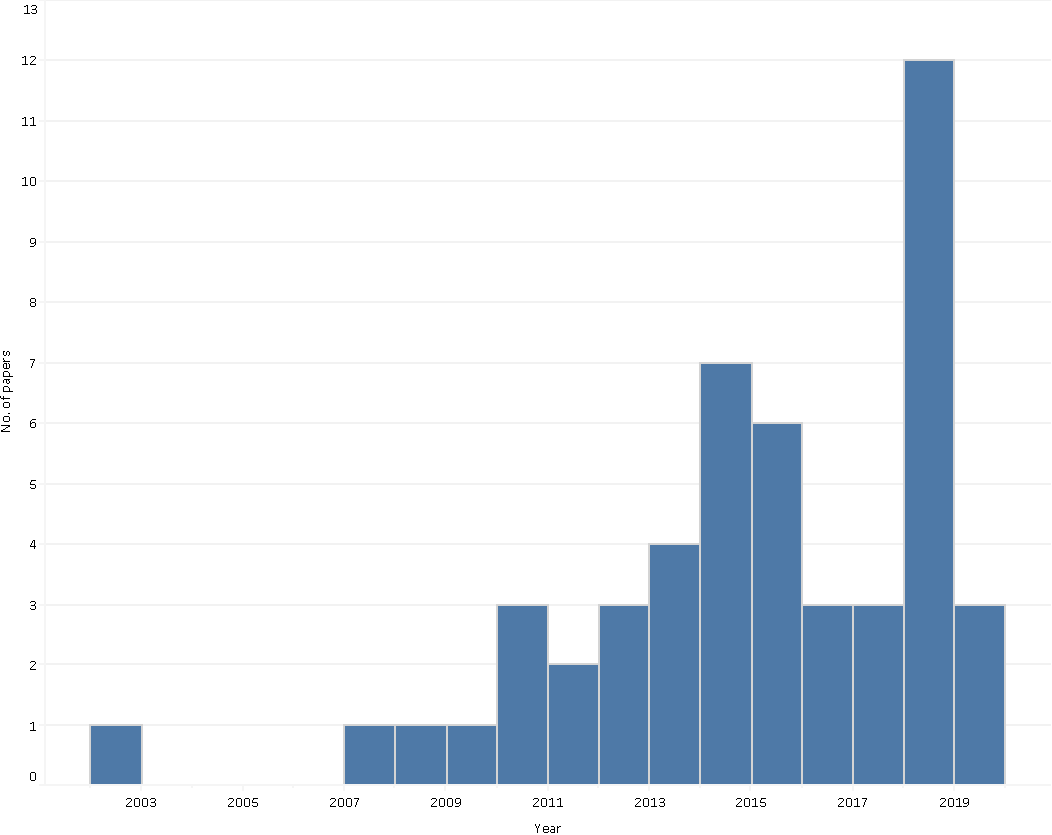
\includegraphics[width=10cm]{figures/yearcitations.pdf}
    \caption{Popularity of Citation recommendation as a field (based on no. of papers published)}
    \label{fig:citationyears}
\end{figure}
\section{Local Citation Recommendation}
The term 'context-aware' recommendation only came into being in 2010 with the seminal He et al. paper~\cite{He2010}. This was the first paper which covered local recommendation (alongside global or context-oblivious recommendation). The same authors followed up this study with a statistical machine translation model in~\cite{He2011}. This idea of using a machine translation model is then taken forward to Huang et al, 2012~\cite{HuangKCMGR12}, where they use the idea that specific keywords in the contexts (source language) are translated to cited documents (target language). Their system, in essence, is a de-facto machine translation system for citation recommendation. 
\section{Embedding-based Approaches}
Embeddings are low-dimensional representations of high-dimensional vectors. 
Mikolov et al~\cite{MikolovSCCD13} was the famous paper that introduced Word2Vec, which is a method of converting words into fixed low-dimensional vectors. This led to the paper by Le and Mikolov~\cite{LeM14}, which extended word vectors to paragraph vectors which could be computed for a set of words or an entire document. 
Paragraph vectors were combined with a graph-based random walk method called DeepWalk (Perozzi et al.~\cite{PerozziAS14}) in Ganguly et al.~\cite{GangulyP17}, which is covered in much more detail in Chapter 5. The aim of this paper was not for citation recommendation, but rather for node classification and link prediction. However, we adapt it for citation recommendation in chapter 5. 

There have been a number of embedding-based approaches in the citation recommendation field. The first one was probably Tang et al, 2014~\cite{TangWZ14}, which used TF-IDF vectors to construct cross-language embeddings for local citation recommendation. Jiang et al.'s two papers (\cite{JiangLL18,JiangYGLL18}) also use embeddings in the context of cross-language citation recommendation, but in the global recommendation area. Cai et al, 2018~\cite{CaiHY18} and Zhang et al, 2018 \cite{ZhangYCD18} (which uses paragraph vectors) are also embedding-based global citation recommendation approaches.

Moving back to local citation recommendation embedding approaches, Huang et al, 2015~\cite{Huang2015} was one of the follow-up papers to Huang et al, 2012~\cite{HuangKCMGR12}. Here, they continue their focus on translation models, but add in distributed word representations of the words and cited documents in the citation contexts (Mikolov et al~\cite{MikolovSCCD13}). 

The Hyperdoc2vec paper~\cite{ShiSZZH18} is one of the most recent papers which use embedding-based neural networks. In this paper, the authors aim to learn two representations of each document -- one by treating it as a citing document and the other by treating it as a cited document. They use the full text of the citing and cited documents and claim that their method works better according to four criteria: content awareness, context awareness, newcomer friendliness, and context intent awareness. This approach is adapted in this thesis due to these features. It will be covered in detail in Chapter 5. 
\section{Topic Modelling, Information Retrieval and Random Walks}
Topic modelling and in particular LDA~\cite{BleiNJ03} have been used in multiple citation recommendation papers (\cite{KatariaMB10, DBLP:Jiang13, NallapatiAXC08, LiuYGSG14}). In this thesis, we use LDA as a baseline.

Information retrieval techniques have also been used in previous papers, from TF-IDF-based text comparison, to BM25. Duma et al's two papers (\cite{DumaKLRC16, DumaLCRK16}) both treat citation recommendation as an information retrieval task, while a few papers like Ebesu et al.~\cite{Ebesu2017} use BM25 as a simple baseline. BM25 plays an important role in the hybrid recommendation system created in this thesis. 

Random walks through a citation graph are used in multiple papers (\cite{JiangLL18, JiangYGLL18, CaiHY18, ChakrabortyMNN15} among others). We use random walks to enrich paragraph vectors in the Paper2Vec approach.
Random walks, LDA and BM25 are explained in more detail in Chapter 3, and used in Chapter 5.

One set of algorithms which we won't cover in this thesis go by the name of \textit{personalised citation recommendation} algorithms. These are algorithms which include the author details and other information such as details of the venue/conference, and use them to get personalised recommendations. These tend to perform better, but there is a degree of bias introduced, and it also requires these details to be provided during the prediction phase. 
These personalised algorithms are common in other types of recommender systems, but Liu et al.~\cite{LiuYY13} was probably one of the first to implement a personalised algorithm for citation recommendation. There have been multiple other personalised approaches based on deep learning recently, including Ebesu et al.~\cite{Ebesu2017} (which includes author information), Yang et al.~\cite{YangZCDMGD18} (which includes venue and author information), Cai et al, 2018~\cite{CaiHY18} and Zhang et al, 2017.~\cite{Zhang2017}
\section{Hybrid recommender systems}
It would be expedient to mention hybrid recommender systems at this point of time. Burke \cite{Burke2002, Burke2007} provides an excellent introduction/survey about hybrid recommender systems. Hybrid recommender systems are systems which take predictions from two or more disparate recommender systems, and combine them in different ways. The famous example for hybrid recommendations is that of combining a collabarative-filtering based recommender and a content-based recommender. 
There are a myriad of ways in which recommendations of two systems can be combined according to Burke~\cite{Burke2002}: weighted, switching, mixed, feature combination, cascade, feature augmentation and meta-level. 

In the citation recommendation context, Hsiao et al.\cite{HsiaoCD15} use a hybrid recommendation system which combines results from two disparate systems.
A two-step process (candidate generation, ranking) to citation recommendation is followed in several papers including Zarrinkalam~\cite{Zarrinkalam2013}, Rokach et al.~\cite{Rokach2013}, Bhagavatula et al.~\cite{Bhagavatula2018} and McNee~\cite{McNeeACGLRKR02}, but these aren't hybrid systems per se -- they only use two different algorithms for candidate generation and ranking.
A hybrid citation recommendation system is built as part of this thesis and is explained in Chapter 5.
    \chapter{Background}\label{chap:background}
This chapter will be divided into two subsections. The first subsection will contain definitions of terms related to citation recommendation. The second subsection explains concepts related to the algorithms used in Chapter 5.

\section{Definitions related to citations and citation recommendation}

\textbf{Citation}: \\
In the context of scientific papers, a citation is a symbolic link from a paper to papers or other external sources it references.

\textbf{Citation context}:\\
A citation context is a set of sentences which contain a reference to an external paper. Citation contexts usually have one or more citation markers, which are defined next.

\textbf{Citation marker/placeholder}: \\
A citation marker is an indicator of the location in the text where a paper has to be cited. Authors uses citation markers to point their readers to other papers which they can read for related information.
Citation markers can be of different forms. They can include the author name and year -- (Smith 2008, p. 1), or the authors and the year -- Padgett and Powell (2012), or just the reference number -- [x].

\textbf{Citing document/paper}:\\
Papers that have citation markers which point to external papers/resources are called citing papers. They contain citation markers which have corresponding entries in the reference section. The reference section contains details about the external papers/resources.

\textbf{Cited document/paper}:\\
Papers which are referenced by other (citing) papers are called cited papers. Citing papers are linked to cited papers through citation contexts and citation markers. Details about cited papers are present in the reference section of the citing paper.

Figure~\ref{fig:citingcitedpaper} shows a citing paper with a few citation contexts. Each of the citation markers in the paper, which are referenced in the reference section, point to external cited papers. 

\begin{figure}
 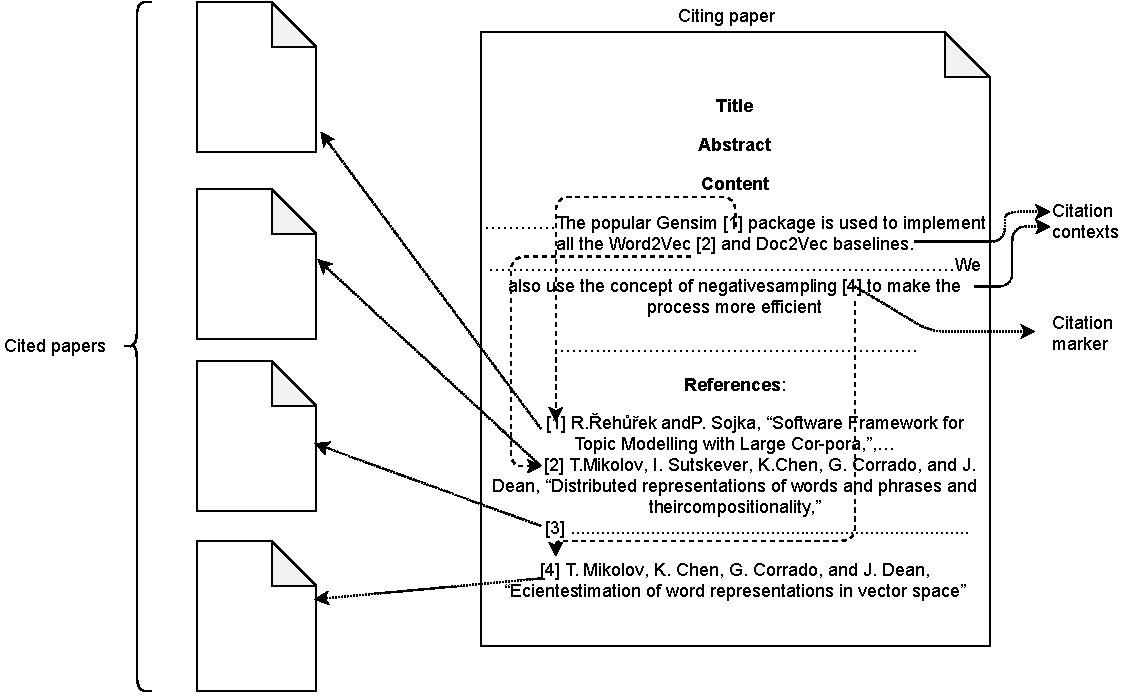
\includegraphics[keepaspectratio, width=13cm]{figures/Background/citedcitingpaper.pdf}
  \caption{Concepts related to citations}
  \label{fig:citingcitedpaper}
\end{figure}

\textbf{Citation Graph}
Citations provide a mechanism by which a set of papers can be visualised in the form of a graph G = <V,E>. Here, the Vertices V are the scientific papers themselves, which contain different citation contexts. There is an edge between two papers if one cites the other. 
A small portion of an example citation graph is shown in Figure~\ref{fig:citationgraph}. In the portion of the graph we're looking at, there are 6 papers published at different points of time. Citation markers (which are part of citation contexts) are shown in square brackets in the figure. A dashed arrow indicates that the paper at the head of the arrow is cited by the paper at the tail of the arrow. So, Paper D cites A,B and C, Paper C cites A and B, Paper E cites A and D, Paper F cites D.

\begin{figure}
 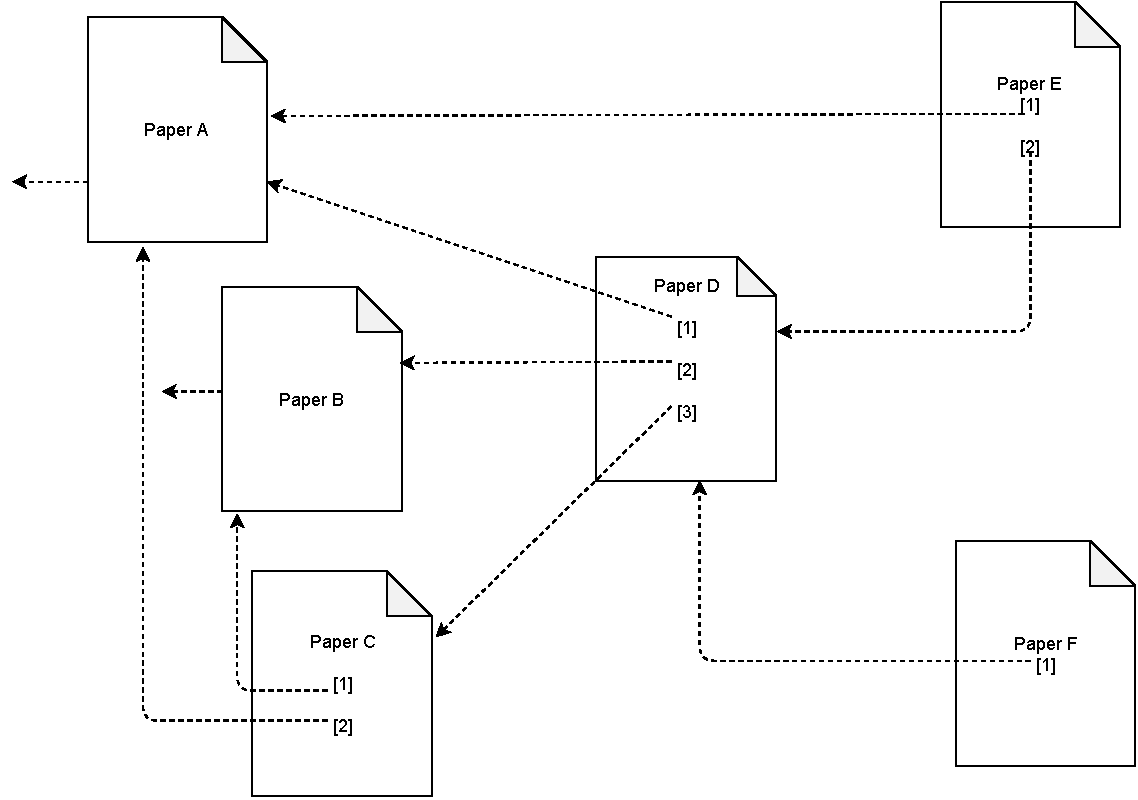
\includegraphics[keepaspectratio, width=13cm]{figures/Background/citationgraph.pdf}
  \caption{Simplified citation graph}
  \label{fig:citationgraph}
\end{figure}
\textbf{Recommender system}: \\
Recommender systems are systems which have the capability of predicting future ratings of items and recommending the predicted items with highest ratings to their users. They are in general either content-based or collaborative filtering-based.
Recommender systems are omnipresent today -- they are used in web searches, e-commerce, paper recommendation, and in a variety of other places. 

\textbf{Citation Recommendation}:\\
Citation recommendation is the process by which cited papers are recommended for citing papers. Citation recommendation can be \textit{global} or \textit{local}. 

In global citation recommendation, references in the reference section are recommended based on the entire content and/or metadata of a paper. 

Local citation recommendation, on the other hand, is the type of citation recommendation in which cited papers are recommended for a citation context. Local citation recommendation can sometimes use metadata along with the citation context as well.

E.g.: Consider the citation context, "The popular Gensim package is used to implement all the Word2Vec and Doc2Vec baselines.". The following recommendations may be retrieved for this context: \textit{Distributed Representations of Words and Phrases
and their Compositionality}\cite{MikolovSCCD13} and \textit{Software Framework for Topic Modelling with Large Corpora}\cite{rehureklrec}.

\textbf{Citation Recommendation System}:\\
This is the actual system used to carry out citation recommendation. If it is a local citation recommendation system, the user of the \textit{citation recommendation system} is recommended a particular number of papers (say, 10) for each citation context.

\textbf{Hybrid Recommender Systems}:\\
Hybrid recommender systems are recommender systems which combine the recommendations of two or more recommenders to return a single set of recommendations.
The combination can be done in a variety of ways: weighted, switching, mixed, feature combination, cascade, feature augmentation and meta-level. These are covered in detail in Burke~\cite{Burke2002}.

\textbf{Weighted hybrid recommender systems}:\\
In a weighted hybrid recommender system, the final scores for an item are computed from the corresponding scores of its composite recommender systems. A weight is assigned to each recommender system to indicate how important it is to the final recommendation. These systems make an important assumption -- \textit{that the relative value of the different techniques is more or less uniform across the space of possible items (entities to recommend)} \cite{Burke2002}. If this assumption is not satisfied, a switching or mixed system might be preferable.
Weighted hybrid recommender systems may use a linear combination of recommender scores, or can use a more complex consensus scheme.


\section{Technical concepts relating to the algorithms}

\textbf{Vector Space Model}\\
The Vector Space Model (VSM) is an important model in the field of natural language processing. In this model, words are converted into vectors. There are different models which are based on the VSM (including word embeddings), but they all follow one basic tenet: words which often occur in the same context are semenatically similar. These words are close to each other in vector space in any vector space model.

\textbf{Bag-of-words Model}\\
A bag-of-words (BOW) model is a common, but simple representation used in information retrieval. Here, a document is represented as a multiset of words. These models do not take the word order into account, but do consider the word frequency of repeated words. So, 'the man has a dog' and 'the dog has a man' will have the same BOW representations.

\textbf{Embeddings}\\
Embeddings are low-dimensional representations of high-dimensional vectors. Embeddings simplify the process of doing machine/deep learning on large inputs. A well-trained embedding places semantically similar inputs close together in the embedding space. Once an embedding is learned, it can be reused across different models.

\textbf{Word embeddings}\\
Word embeddings are embedding models which map words or phrases into numerical vectors. These vectors can be generated by different methods such as neural networks and probabilistic models. 
Word embeddings have become increasingly important in the field of natural language processing. Some popular deep-learning based word embedding models include Word2Vec \cite{MikolovSCCD13}, GloVe \cite{pennington2014glove}, FastText \cite{BojanowskiGJM16} and ELMo \cite{Peters:2018}. 

\textbf{Cosine Similarity}\\
Cosine similarity is a similarity measure used to measure the angle between two non-null vectors. It is very commonly used to compare two word vectors produced by embedding models. The smaller the angle between two word representations, the closer they are semantically. 

\textbf{Softmax}\\
In a multi-class algorithm (which is one lens through which we can look at citation recommendation), a softmax function returns probabilities for each output class.

\textbf{Word2vec}\\
Word2Vec \cite{MikolovSCCD13} is an efficient neural network-based model to compute vector representations for words. John Rupert Firth, the great English linguist, famously said, \textit{"You shall know a word by the company it keeps"}. This is the principle by which Word2Vec works. Words are predicted based on their surrounding words. 

As a result, it can be used to find synonyms and words with the same semantic relations. The stereotypical Word2Vec example shows the 'gender' semantic relation. This oft-repeated example is King: Queen, Man:?. 
Word2Vec throws up 'Woman' as the vector having the closest relation (angle) to 'Man' as 'Queen' has to 'King'. This happens because they are used in similar contexts. 

The neural network model that Word2Vec uses has an input layer, a single hidden layer and a softmax classifier as the output layer. 
The trick used in Word2Vec is that the weights of the trained neural network can be used for other tasks. Here, the size of the hidden layer is the size of each word vector. Each of the rows of the hidden layer's input weight matrix corresponds to individual word vectors. In this thesis, these word vectors will be referred to as IN word vectors. OUT word vectors come from the weights matrix between the hidden and output layers. 

OUT vectors are not generally used, but Nalisnick et al.~(\cite{NalisnickMCC16}) posit that comparing two IN vectors (IN-IN), two OUT vectors (OUT-OUT) or an IN and an OUT vector (IN-OUT) have different meanings semantically.

\textbf{Word2Vec: CBOW and Skip-Gram}\\
Word2Vec has two different flavours: Continuous Bag of Words (CBOW) and Skip-Gram. In CBOW, the target word is predicted from the surrounding source words. The window size for the number of surrounding words has to be defined. For example, consider the following sentence: 'Xi is the President of China' and a window size of 5. Here, each word is predicted in turn based on the surrounding words. After 'Xi' is predicted from  ('is', 'the', 'President', 'of', 'China'), the window slides, and the next word is predicted from its neighbours.

The Skip-gram model flips things around. Here, the surrounding words are predicted from the 'centre' word, i.e. the neighbours are predicted based on a single word. Using the same sentence as an example, the word 'China' would \textit{predict the words ('Xi', 'is', 'the', 'President', 'of'}.

For both the models, the surrounding words form a \textbf{context window} and the number of surrounding words is a hyperparameter which has to be defined.
Another important hyperparameter is the acual size of the word vectors.

\textbf{Paragraph vectors (Doc2Vec)}\\
Mikolov and Le's extension of their Word2Vec paper \cite{MikolovSCCD13} resulted in the concept of paragraph vectors \cite{LeM14}. This has been popularised as 'Doc2Vec' by the Gensim package \cite{rehureklrec}. A paragraph vector is a vector which represents the meaning of a paragraph or a whole document. 

Just like Word2Vec, Doc2Vec is trained using a similar neural network with a single hidden layer. In this thesis, we refer to the vectors from the weight matrix betweeen the input and hidden layers as the IN document vectors. The vectors from the weight matrix between the hidden and output layers are called the OUT document vectors.

\textbf{Doc2Vec PV-DM and PV-DBOW}\\
The PV-DM (Distributed memory version of paragraph vectors) is an extension of the CBOW model. Here, word vectors in the context are combined (averaged/concatenated) with a special paragraph ID to predict the centre word. 

The PV-DBOW (Paragraph Vector- Distributed Bag of Words) model is an extension of the Skip-gram model. Here, an individual document vector is used to predict the words in the document. 

Like Word2Vec, the size of the context window and the vector size are important hyperparameters. 

\textbf{Sampling rate}\\
The sampling rate is an important hyperparameter for Word2vec and Doc2Vvc which indicates the probability with which a word is kept in the vocabulary. Higher sampling rates result in many frequent words being removed from the vocabulary. 

\textbf{Negative sampling}\\
Negative sampling \cite{MikolovNegsamp} is a method used to make the training of Word2vec and Doc2vec models more efficient. While training the neural networks, only certain weights of the output layer are updated for each training example. Some negative samples are chosen for each word (words which do not often occur together are negative samples). The weights for these negative words (say, 5) and the positive word are the only weights updated, and the rest of the weights are not touched.

\textbf{Topic Modelling}\\
Topic modelling is used to discover abstract topics that occur in a collection of documents. It assigns topics to each document, such that similar documents will have a number of common topics.

\textbf{Latent Dirichlet Allocation}\\
The Latent Dirichlet Allocation (LDA) \cite{BleiNJ03} is a popular topic modelling technique which we will use as a baseline in this paper. In LDA, a document is described by a distribution of topics and a topic is described by a distribution of words. 

\textbf{Hyper-document}\\
In Han et al (\cite{ShiSZZH18}, the authors define what they call a hyper-document. A hyper-document is a collection of words and document IDs, with the document IDs substituting for citation placeholders. Consider a citing document $d_s$, which cites a document $d_t$. Let the words in the citation context be C. Then the document $d_s$ is a hyper-document which has a hyperlink <$d_s, C, d_t$>.

\textbf{Random walk}\\
A random walk in a graph is a succession of random steps in the graph. This stochastic process results in a random path being described, as well as a random destination node being reached.

\textbf{DeepWalk}\\
DeepWalk is a popular algorithm for learning node embeddings introduced by Perozzi et al (\cite{PerozziAS14}). They treat nodes as pseudo-words, and the training process is hence similar to training word embeddings. They first perform random walks on nodes in the graph. The resulting node sequences are run through the Skipgram algorithm (also used in word2vec) to get the final embeddings.

\textbf{Genetic algorithms}\\
In general, genetic algorithms are "stochastic search and optimization algorithms that mimic natural selection to find a good solution" \cite{Mueller17}. These algorithms use analogies from microbiology -- the terms to draw from are called chromosome pools. 
Genetic algorithms cover a succession of steps, as explained in \cite{Mueller17}:\\
1. Initialize Population: A random population of chromosomes is created from the chromosome pool.\\
2. Fitness score: the 'fitness' of each chromosome is evaluated using a function.\\
3. Selection: A random selection with replacement is made from the population of chromosomes based on the fitness score.\\
4. Cross-over: Pairs of chromosomes are mated -- parts of their chromosome information are exchanged.\\
5. Mutation: A low probability that some of the chromosomes may be altered or replaced is introduced.\\
6. Solution Set: Once the stopping condition is reached (when a certain fitness score is reached/a particular number of iterations is reached), the chromosomes that are left form the solution set.
    \chapter{Data sets}\label{chap:dataset}

The amount and quality of data used for training a deep learning/machine learning model is arguably more important than the quality of the actual algorithms used. So the preparation of the input data is a critical step in the whole process. 
In the following section (4.1), we will discuss 4 existing data sets which are used as 'base' data sets. In Section 4.2, we will talk about the data preparation phase. In this phase, the base data sets are combined and made into a form usable for the approaches described in Chapter 5.

\section{Description of base data sets}
Four data sources are used in this thesis: MAG, Arxiv, ACL-ARC and Unpaywall. Details about the specific versions of the data sets that we use are given in Appendix~\ref{chap:offlineevalfilter}. These four 'base data sets' are described below.
\subsection{The MAG Data set}
The Microsoft Academic Graph data set (MAG), a relatively new data set, has close to 220 million papers by 240 million authors (as of 22 May 2019). Papers in the data set range all the way from 1800 to 2019. \footnote{Latest statistics for Microsoft Academic can be found at https://academic.microsoft.com/home}. MAG was created using a combination of automatic crawling (using Microsoft's search engine Bing), and manual file sourcing from different sources (publishers like ACM) \cite{Sinha2015}. MAG gets monthly updates, leading to an ever-increasing amount of paper coverage. 

These papers encompass many different disciplines (fields of study in MAG parlance) and languages. As per Microsoft's 2015 paper \cite{Sinha2015}, the Microsoft Academic graph is modelled as a "heterogeneous graph consisting of six types of entities: field of study, author, institution (affiliation of author), paper, venue and event". The links between the entities are explained in the same paper. Since then, more entities have been added, including paper URLs and paper resources.  

Furthermore, MAG supplies files containing individual citation contexts, with the citing and cited papers' internal MAG identifiers provided alongside. Also provided are files with references, abstracts and language indicators for the papers. A detailed analysis of the MAG data can be found in \cite{Herrmannova2016}, while \cite{Paszcza2016} compares MAG to other scholarly databases. An analysis of the citations in MAG has been carried out in \cite{Hug2017}. 

All the data and metadata are provided by Microsoft in the form of monthly dump files on Azure, its cloud computing system. The dump files will be used in the data preparation phase, the phase which makes the data usable by the recommendation algorithms. The data preparation for MAG is described in Section 4.2.2. 

There are a number of reasons why we think MAG will be used extensively in research. Apart from the huge amount of coverage across a myriad of disciplines (fields of study), there is a possibility to drill down into sub-disciplines for most of the papers. There are papers from multiple languages, and a comprehensive amount of metadata about authors, journals, conferences, affiliations etc. The additional presence of citation and reference information facilitates research into citation recommendation, along with other research fields like paper recommendation, bibliometrics and scientometrics. The one downside to using MAG has is that full text is not provided for any papers. When needed, this has to be obtained from other sources. However, the pros of using MAG (data from many disciplines, availability of citation and reference information, and the sheer amount of metadata) outweigh the cons. This thesis therefore built around this data set.

In the citation recommendation context, the 2015 version of the MAG data set, just called Microsoft Academic, was used to get citation recommendations from a set of keywords in Chakraborty et al.\cite{ChakrabortyMNN15}. It was also used in Gao et al.~\cite{Gao15}, in which the impact of time on citation recommendation is studied by creating TF-IDF vectors and author profiles. Both these papers, however, do not consider the problem of context-aware citation recommendation. They also do not use the citation contexts provided in MAG.
\subsection{Arxiv}
Arxiv \footnote{https://arxiv.org/}, an initiative by Cornell University, provides open access to the full text of papers from  mainly 5 disciplines -- mathematics, computer science, physics, biology and economics. While citation contexts are not directly available, the full text in PDF as well as \LaTeX files can be obtained from Arxiv. 

Although Arxiv does not quite match the breadth of coverage in MAG, it still contains a substantial number of papers. 
The total number of submissions, as of 22 May 2019, is over 1.5 million \footnote{current stats available at https\://arxiv.org/stats/monthly\_submissions,\, https\://arxiv.org/help/stats}. 

The authors of \cite{SaierF19} have extracted the plain text from the aforementioned \LaTeX source files. This is the version of Arxiv data that will be used in this thesis. Their \LaTeX extraction process is described in brief in Section 4.2.3, along with the final data preparation process (which includes combining Arxiv and MAG data) for the approaches in Chapter 5. At the end of their process, we get full text which is clean. This is in contrast to the MAG, where we don't have full text, and the data is not always clean. 
\subsection{ACL Anthology}
The ACL Anthology Reference corpus (ACL-ARC) is a comparatively tiny dataset which covers only computational linguistics and natural language processing. It contains close to 11,000 papers and stretches from 1965 to 2006. The ACL data we use for the thesis has been preprocessed as per \cite{Faerber2018} to contain a set of sentences, with references and metadata available in a separate file. This is further described in Section 4.2.4, which covers the data preparation phase for the ACL data and the process of combining it with MAG.
\subsection{Unpaywall}
Unpaywall \footnote{https://unpaywall.org} is a cross-domain open source database of 23,268,544 scholarly articles (at the time of writing). The organisation responsible for Unpaywall also provides a freely-downloadable database snapshot every few months in the Jsonlines format \footnote{https://unpaywall.org/products/snapshot (snapshot used: September 2018)}. 
The Jsonlines file has a JSON record for each paper, with each record containing the paper's DOI and some other metadata, along with links from which the papers can be freely downloaded. The DOI can be used to link the papers in this Jsonlines file to other data sets such as MAG. The data preparation using Unpaywall and MAG is covered in Section 4.2.5. 
\section{Data set preparation}\label{sec:data-set-creation}
In this section, we will take a look at the methods behind the creation of the the final data sets from the base data sets described in the previous section. The first thing we do is to restrict the data sets to only computer science papers. There are multiple advantages to using only one discipline -- the recommendations are likely to be better, and the training time for the embedding-based algorithms is reduced. The price we pay is that we miss out on cross-domain recommendations. 

The full-text base data sets (Arxiv, ACL-ARC, Unpaywall) are supplemented with additional content from MAG. This content is made up of what is referred to in this thesis as \textit{'pseudo full-text'}. The pseudo full-text for a paper consists of its title, abstract and all its citation contexts (i.e., citation contexts where it acts as a citing paper) from MAG. This is done so that we have at least some content for papers which have been cited by the papers in the full-text base data sets, but which are not in the respective base data sets themselves. 

The process to create the MAG pseudo full-text, which is common to the data preparation phases of all the full-text data sets, is described in Section 4.2.1. The data preparation phases for the individual data sets are explained in Sections 4.2.2-4.2.5.

Two additional data sets based on the MAG are created for evaluation. These data sets are called MAG50 and MAG-Cited, and they are explained in Section 4.2.6. These two data sets also play a big role in the final running recommender system, \textit{HybridCite}, which is described in the next chapter.

The end result after the data preparation phase is a single training file for each of the data sets. All the training files have citation markers of the form $=-=$MAG ID$-=-$, as all the papers in even the non-MAG data sets are mapped to MAG IDs.

Table~\ref{tab:MAGdatasets} contains some details about the training sets created for the MAG data sets (the main MAG data set, MAG50 and MAG-Cited). 
Table~\ref{tab:nonmagdatasets} gives an overview of the training sets created from the full-text data sets in conjunction with MAG (pseudo full-text extracted from MAG).
The filter criteria used to prepare these data sets are explained in detail in Appendix~\ref{chap:offlineevalfilter}.

\textbf{Note about test set preparation}:
A test set containing citation contexts is also created for each of the data sets. All the test set citation contexts are extracted from the respective data source (Arxiv/ACL AAN/MAG), and are subject to a few filter criteria as well. In addition to the filter criteria used for creating the training sets, each of these test contexts must have at least 9 words after removing stop words. We remove stop words quite aggressively, based on \cite{StoneDK11}. All the stop words removed are given in \ref{chap:preprocessing}.

\begin{table}
\centering
    \begin{tabular}{ccc}
    \toprule
    Data set & \#Papers & Years \\
    \midrule
       MAG & 1,620,841 & 1800-2017 \\
       MAG50 & 126,666 & 1800-2017 \\
       MAGCited & 1,629,106 & 1800-2017\\
    \bottomrule
    \end{tabular}
    \caption{Overview of MAG training sets (after data preparation phase). Filter criteria used for the data preparation can be found in Appendix~\ref{chap:offlineevalfilter}.}
    \label{tab:MAGdatasets}
\end{table}

\begin{table}[]
    \centering
    \begin{tabular}{ccccc}
    \toprule
    Data set & \#Papers & \#Full-text papers & \#Pseudo full-text papers & Years \\
    \midrule
        ACL-MAG & 11,217 & 9,166 & 2,051 & 1965-2005 \\
        Arxiv-MAG & 286,272 & 53,614 & 232,658 & 1991-2016 \\
        Unpaywall-MAG & 1,185,090 & 397,687 & 787,403 & 1800-2017\\
        \bottomrule
    \end{tabular}
    \caption{Overview of training sets which include full-text from the respective data sources and pseudo full-text from MAG. Filter criteria used for the data preparation can be found in Appendix~\ref{chap:offlineevalfilter}.}
    \label{tab:nonmagdatasets}
\end{table}

\subsection{MAG \textit{Pseudo full-text} preparation}
Since the MAG data set does not contain full text but contains citation contexts and plenty of metadata, a mechanism is needed to combine the contexts and metadata into a form usable by the algorithms in Chapter 5. So, the title, abstract and citation contexts are retrieved for each paper and concatenated to form text which acts as a substitute for the full text (hence the name, \textit{pseudo full-text}). 

For each citation context, the MAG ID of its cited paper is inserted at its mid-point. If a citation context has 11 words, the citation marker is inserted after the 5th word. The reason that this has to be done is that the MAG citation data contains only one reference ID (cited paper ID) per citation context. If a citation context cites 2 papers, duplicate rows are present in the MAG citation data, each with one cited paper's reference ID associated with it. As there is no way to figure out which citation marker a reference ID corresponds to when there are two or more citations, we simply insert the reference ID at the mid-point of the context. 

In case of the non-MAG data sets, the data preparation phase involves mapping to MAG, and getting additional data of papers cited in the respective data sets. For example, an Arxiv paper (with full text available) might cite a total of 10 papers, out of which only 2 are within the Arxiv data set. Let's assume 6 of the remaining 8 papers have data available in MAG. We map these papers to MAG (the specific mapping methodology is different according to the data set, and is explained in the respective subsections), from which we get their title, abstract and the citation contexts. These fields are concatenated to form psuedo full-text.

The newly-obtained citation contexts in turn reference other papers within the MAG database. Again, the respective MAG IDs of these papers are inserted as citation markers at the exact mid-point of the respective citation context.  

The reason we go through this process to get the pseudo full-text is that one of the embedding algorithms used in Section 5 (Hyperdoc2vec) requires representations for every citing and cited paper. This algorithm creates two types of embeddings -- one based on citation contexts and the other based on content, so we require the title and abstract (to use as content) as well as the citation context in the pseudo full-text. 

Pseudo full-text plays an important role in training all our algorithms. Table~\ref{tab:nonmagdatasets} shows that two of the prepared non-MAG data sets finally contain more pseudo full-text papers than full-text papers.
\subsection{MAG}
To prepare the MAG \textbf{training set}, the dump files mentioned in Section 4.1.1 are first loaded into several PostgreSQL tables. From the PostgreSQL tables, the pseudo full-text (title, abstract and concatenated citation contexts) is prepared for each paper as described in Section 4.2.1. 
All the algorithms, whether embedding-based, information retrieval-based or topic modelling-based, work better when there is as much text as available. While having the full text would have been ideal, MAG does not contain full text. Therefore, using the title and abstract with all the citation contexts as pseudo full-text is the best we can do.

We do not use the entire MAG data for creating the training set. We use only computer science papers in English from 1800-2017 because this is a discipline which is familiar to the writer, and has a relatively large number of papers. A few other filter criteria are applied as well while preparing the training set. These filter criteria are explained in Appendix~\ref{chap:offlineevalfilter}.

The \textbf{test set} uses citation contexts from computer science papers in English which were published in 2018 and 2019. The MAG citation contexts are not always clean, and a few unclean contexts do get through the cracks into the test set (as well as the training set). These contexts are best avoided, and a machine learning algorithm with handcrafted features was developed to discard 'incomplete' contexts. However, the machine learning algorithm was trained on a small set of citation contexts with manually selected labels. It wasn't clear if it would work well on a large amount of data or if it would generalise across the computer science sub-fields, so this ML algorithm was not applied.

These incomplete contexts bring down the metric scores when the evaluation is done, but this can only be partially prevented. The restriction mentioned in the previous subsection is imposed: citation contexts with 9 or fewer words (excluding stop words) are not included. The papers which are not present in the training set are discarded as well.  

The MAG citation data has a citing and cited MAG ID associated with each citation context. The cited MAG ID acts as the ground truth. As mentioned in the previous section, this citation data has separate (duplicate) records for contexts with two or more citation markers. In the test set preparation, these contexts are grouped (by the paper id and the context) resulting in a single record with multiple cited papers in the ground truth. 

\subsection{Arxiv-MAG}
Saier et al \cite{SaierF19} present an approach to convert \LaTeX source files provided by Arxiv into text files. They extract the text into text files and create a database in which they map the papers in the reference section of each paper to MAG. They also obtain the precise positions of the citation markers corresponding to each of the references in the paper text, and insert placeholders with unique IDs at these locations.

These text files and the aforementioned mapping database act as the starting point for the preparation of the Arxiv-MAG \textbf{training file} in this thesis. The MAG ids from the references database are inserted at the positions in the Arxiv text files with unique IDs, replacing the citation placeholders. Arxiv provides a metadata file \footnote{https://arxiv.org/help/bulk\_data}, which is indexed in Apache Solr \footnote{https://lucene.apache.org/solr/} at this stage.

A couple of filter conditions are applied on the data set of Arxiv papers -- only computer science papers from 1991-2016 are considered, and papers which have been cited less than five times are discarded. Appendix~\ref{chap:offlineevalfilter} shows all the filter criteria.

As our final data set will contain additional data from MAG (pseudo full-text), it is necessary to map all the Arxiv IDs to MAG IDs. The title and published year are retrieved from the Arxiv Solr metadata index for each of the papers in the Arxiv corpus. These fields are normalized, and mapped to the MAG metadata tables by performing an exact match on the paper title and published year. If there is no match, another attempt is made to map just the Arxiv title to the MAG metadata title. All the Arxiv papers which cannot be mapped to MAG are not included in the training set. 

Pseudo full-text is fetched from the MAG tables for the cited papers which are not within the reduced Arxiv data set, as explained in Section 4.2.1. This pseudo full-text includes only those citation contexts which cite papers within either the reduced Arxiv data set or the set of papers which the original Arxiv papers cite.

To prepare the \textbf{test set}, citation contexts of computer science papers from 2017 are extracted from Arxiv. Like in the training set, the Arxiv IDs of the cited papers are mapped to MAG IDs, and act as the ground truth. The ground truth contains one paper in most cases, but can have one main reference, and possible 'adjacent' references. These adjacent references are ones that are at most 5 characters apart or are part of a group of citations. ”[25,26]”, ”[25], [26]” or ”[25] and [26]" are examples of cases where adjacent citations are present. Again, references which are not in the training set are discarded from the ground truth.  
\subsection{ACL-MAG}
In \cite{Faerber2018b} and \cite{Faerber2018}, the authors describe a method to detect citation contexts from ACL Anthology (and Arxiv) papers. They also provide the data for \cite{Faerber2018b} online \footnote{\url{http://citation-recommendation.org/publications/}}. In this data, they have obtained the references of each paper and mapped them to GC/DBLP.  The data has been divided into 3 files for each paper: a text file containing text and annotations for citation markers, a references file, and a metadata file. 

To create the \textbf{training set}, we make use of just the text files and consider only the annotations which have been mapped to DBLP. The method to get the MAG ID in place of the DBLP annotations is described below. The text files are iterated through and the DBLP URL is obtained from the DBLP annotations. This DBLP URL is scraped, and the paper's title is obtained. This title is used to map to MAG in the same way as for Arxiv in Section 4.2.3. The annotations are replaced by the MAG IDs to obtain the full text. The training data contains all papers from 1965 to 2005.
Again, additional MAG pseudo-text is added for these papers' reference papers, as described in Section 4.2.1.

The \textbf{test set} contains contexts from ACL Anthology papers in 2006. The papers in the ground truth are fetched from the references and mapped to MAG in the same way as the training set. Any papers not in the training set are removed from the ground truth. Unlike Arxiv, all the test set contexts have only one paper in the ground truth. 
\subsection{Unpaywall-MAG}
The steps to prepare the \textbf{training data} from the Unpaywall JSONlines is described below. The DOIs in the Unpaywall JSONlines file are mapped to the MAG metadata tables directly and a mapping table is created. The Unpaywall JSON file has links from which the papers can be downloaded. Only DOIs which belong to papers from the computer science field of study in MAG, and written in English before 2018, are included in the mapping table.

The required PDFs are downloaded using a program and stored. The GROBID \cite{GROBID} tool is then executed on the PDF files to convert them to tei.xml files. GROBID parses PDFs and finds references authomatically. The tei.xml files contain the full text with references replaced by generated reference IDs. These IDs are mapped to bibliographic data in the references section of the tei.xml files. 

These tei.xml files produced by GROBID are iterated through and a single text file for all the data is produced in which the references are replaced by the respective MAG IDs. The MAG IDs are obtained, like in the case of Arxiv-MAG, by mapping the title and published year to the MAG metadata.
Additional pseudo full-text data from MAG is added to the file using the same method as the other non-MAG data sets.

The \textbf{test file} used is the same as the test file used for MAG in Section 4.2.2.

\subsection{Additional MAG Data sets}

\subsubsection{MAG-50}
The data preparation is very similar to the normal MAG data set (see Appendix~\ref{chap:offlineevalfilter}), but only those papers which have at least 50 citations are included in the training set. This considerably reduces the total number of total papers in the prepared training set, but will produce better results using the approaches described in the next chapter. However, this means that papers without citations (for example, new papers) will never get recommended. This data set is used to do a case study comparing the results to the main MAG data set where no restriction is made on the number of citations. It is also used in the final recommender system.

\subsubsection{MAG with cited contexts (MAG-Cited)}
\cite{HuangKCMGR12} and \cite{Huang2015} claim that "a citation’s context contains explicit words explaining the citation". They say that the words in the context explain the cited paper rather than the citing paper. This thesis also does a small case study to prove this claim by creating the MAG file in a similar way to Section 4.2.2. But instead of using each paper's own citation contexts in its pseudo full-text, citation contexts from papers which cite the paper are used. For example, consider a situation wherein a paper A cites two papers B and C, but A is \textit{cited by} 3 other papers D, E and F. The content of A is made up of A's title and abstract, and citation contexts from D, E and F which reference A (unlike the data set in Section 4.2.2 which would have A's title and abstract and citation contexts).
    \chapter{Approach}\label{chap:approach}

Citation recommendation, like so many other fields in computer science, has been taken over recently by deep learning/neural networks. There are approaches which use different types of RNNs~\cite{Kobayashi2018, YangZCDMGD18} and CNNs~\cite{Ebesu2017, YinL17}. But in the context of this thesis, we are more interested in approaches which use the concept of embeddings in some form or the other. Embeddings have been used in both global and local citation recommendation, as explained in Chapter 2. 
The global recommendation approaches include  \cite{JiangLL18}, \cite{JiangYGLL18}, \cite{CaiHY18} and \cite{ZhangYCD18}. 
In the local citation recommendation field, which is our focus, \cite{TangWZ14} and \cite{Huang2015} are two examples. 

In this chapter, we will look at a number of potential component algorithms which might be used in the final hybrid recommendation system. We start by describing two methods of generating embedding vectors. 
Paper2Vec~\cite{GangulyP17}, one such embedding approach which combines document vectors (paragraph vectors) with random walks, is discussed in Section 5.1. While the authors of the Paper2Vec paper use it for other purposes, it is adapted for citation recommendation here.
Hyperdoc2vec~\cite{ShiSZZH18}, whose purpose is to generate task-independent embeddings of hyper-documents (documents with either hyperlinks or citations links to other documents within their text). Hyperdoc2vec is described in Section 5.2. Section 5.3 covers 2 approaches initially earmarked as baselines: citation recommendation using topic modelling (LDA) and information retrieval (BM25). 

A semi-genetic hybrid algorithm is presented in Section 5.4, which combines the recommendations from BM25 and Hyperdoc2Vec stochastically, and returns a new list of recommendations. 

An improved hybrid algorithm called Hybrid23 is described in Section 5.5. This algorithm exploits two data sets at the same time to improve its recommendation performance. While the first data set is the normal MAG data set (described in Section 4.2.2), the second data set (MAG-Cited, described in Section 4.2.6) is the one which makes a lot of difference in the recommendation quality. Hybrid23 is used in the running recommender system, which is described in Section 5.6. 
\section{Paper Embeddings: Paper2Vec}
The Paper2Vec paper by Ganguly et al~\cite{GangulyP17} provides a mechanism to produce document vectors (paragraph vectors~\cite{LeM14}) enriched by random walks. Their algorithm learns embeddings by combining text information and citation information in two distinct steps. These embeddings are later used for our purpose of citation recommendation. 
\subsection{Training process}
A two-step process is described in the original paper. This is explained in brief here, along with an additional intermediate step. The flowchart in Figure~\ref{fig:p2vtrain} shows the entire process. 

In the first step, document and word vectors are produced for all the papers in our corpus using the Gensim package \cite{rehureklrec}. 
For this, the Skip-gram algorithm is used to learn word vectors, and the pv-dm algorithm~\cite{LeM14} is used to learn document vectors. According to the authors of Paper2Vec, pv-dm~\footnote{Chapter 3 explains pv-dm, pv-dbow and Skip-gram} worked better than pv-dbow. The Gensim package for this is called Doc2vec, and when used with pv-dm, it produces a set of document vectors for all the papers in the training set, and a set of word vectors for the words in the training set. Negative sampling is used to make the training more efficient. 

It is vital to note that neither the citation markers nor the citation links contribute to the produced vectors at this stage. The first step is essentially a content-based Doc2Vec embedding. The preprocessing done is making words lower-case, removing stop words, expanding contractions and removing extra white spaces (see Appendix~\ref{chap:preprocessing} for more details and the complete stop word list).
\\
The pv-dm training step proceeds as follows. A sliding window of size 10 is used, and each word in this window is predicted by averaging the word vectors of the surrounding words and the document vector. This is repeated after sliding the window multiple times through the document, reducing the loss in each step using stochastic gradient descent. For each word in each window, the average log probability is maximised using the multi-class softmax function as given by the following equation.
\begin{equation}
    P(w_j|{w_i, d_k}) = \frac{exp(w_j^Tw_i + w_j^td_k)}{\sum_{t=1}^{C_1}{exp(w_t^Tw_i + w_t^Td_k)}}
\end{equation}
Here, $w_j$ is the word vector to be predicted from the surrounding word vectors $w_i$ and document vector $d_k$.

So we maximise the following equation: 
\begin{equation}
    \sum\limits_{w_i, w_j \in c_1}^{|C_1|} log P(w_j|{w_i, d_k})
\end{equation}
Figure~\ref{fig:pvdm} shows the pv-dm process for an example window size of 3. Here, a word 'paragraph' is predicted from the document vector for the citing paper Le and Mikolov (2012) and the words surrounding 'paragraph'. This is repeated for every word through a stochastic gradient descent to train the algorithm.
At the end of Step 1, the hope is that papers whose content is semantically similar are close together in the vector space. 
\begin{figure}
\centering
 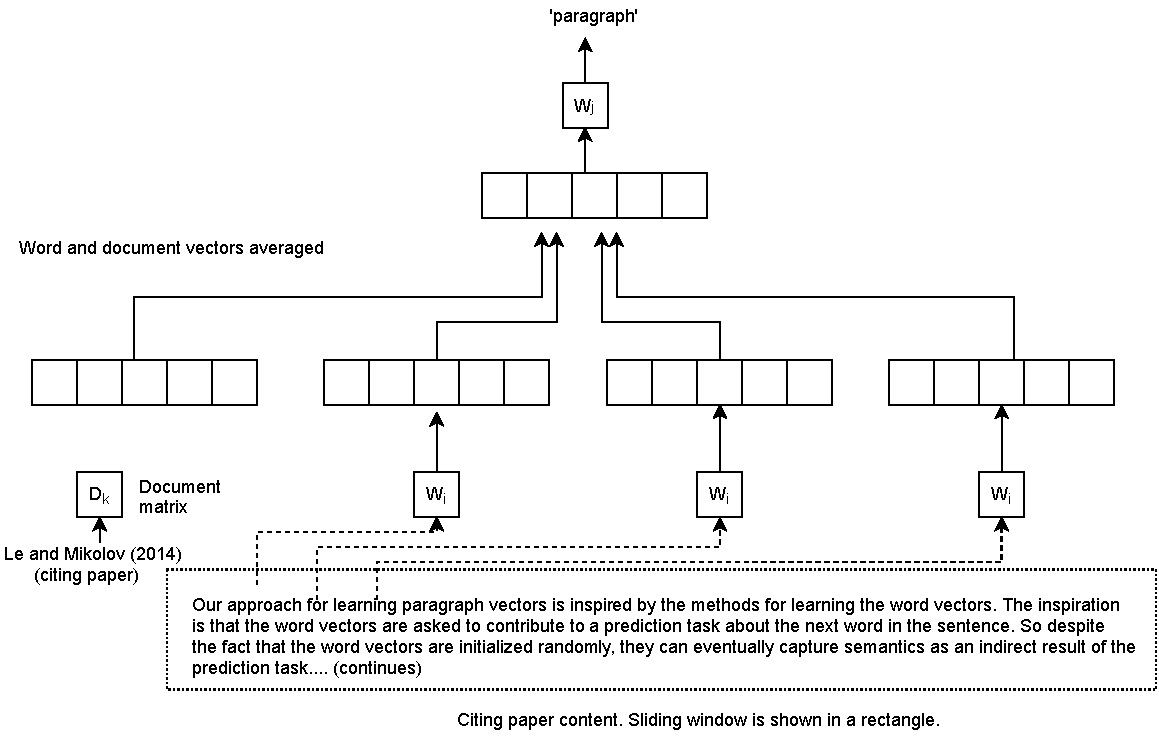
\includegraphics[keepaspectratio, width=13cm]{figures/Approach/pvdm.pdf}
  \caption{Step 1 of Paper2Vec \cite{GangulyP17}: framework for the Doc2vec (pv-dm) model}
  \label{fig:pvdm}
\end{figure}
Before starting Step 2, an intermediate step is carried out in which the set of references for every paper in the training set are obtained. Any references which are not contained within the set are removed. This set of references is obtained during the data preparation phase of Arxiv-MAG, Unpaywall-MAG and ACL-MAG as a by-product. For the MAG data sets, the references are obtained directly from a table containing paper references. These references form a citation graph G = <V,E> with a link appearing between two papers when one cites the other. These edges are assumed to be undirected. So, A citing B is equivalent to B citing A.

\begin{figure}
\centering
 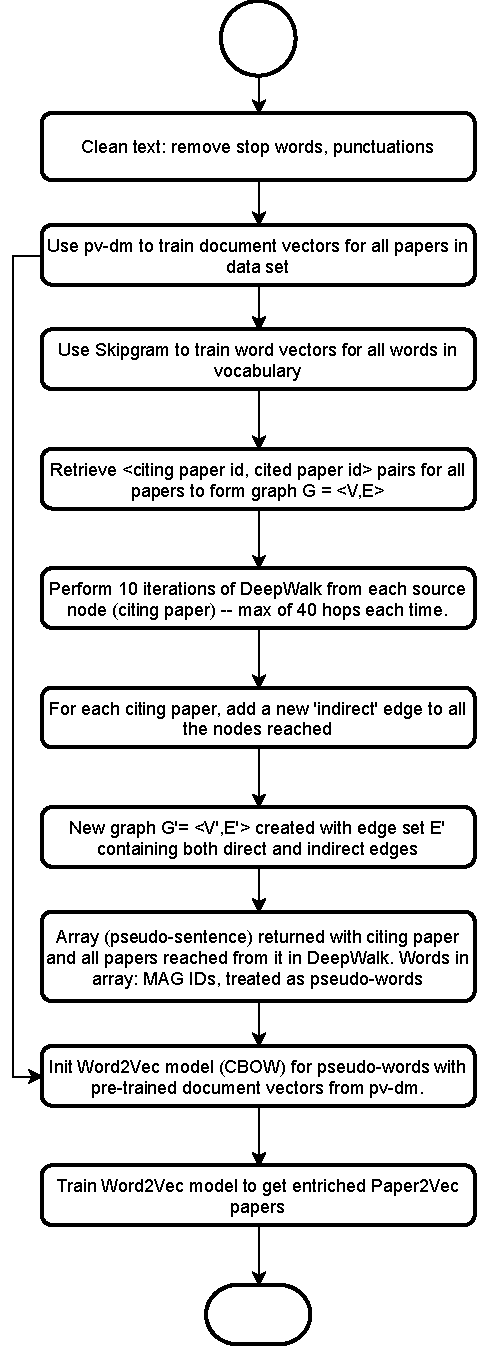
\includegraphics[keepaspectratio, width=8cm]{figures/Approach/paper2vecflowchart.pdf}
  \caption{Flowchart: Paper2Vec~\cite{GangulyP17} training process}
  \label{fig:p2vtrain}
\end{figure}
The document vectors are enriched in Step 2 by creating additional links between the papers through a random walk (based on DeepWalk \cite{PerozziAS14}) step. The graph from the intermediate step contains a number of edges (one edge for each citing-cited paper link)in set E. DeepWalk uses two hyperparamteters for its random walk step: 'number of walks', and 'path length'. 
The 'number of walks' hyperparameter indicates how many times the random walk process should run for a citing paper. The 'path length' hyperparameter indicates how many hops are made in one random walk (DeepWalk) step. Path length is set to 40 and number of walks is set to 10 for all the data sets used in this thesis.

DeepWalk works as follows. The source node (citing paper) of each edge is taken as a starting point and a maximum of 40 hops are made (if an unconnected node is reached, the random walk process ends). This is repeated for 10 iterations. All the nodes reached are returned as an array, and an edge is created between the citing paper (source node) and the nodes reached from it in the 10 DeepWalk iterations. \\
So the new graph at this point is G' = <V, E'> with E' containing the edges in E and all the new edges created during the DeepWalk process. For each citing paper, DeepWalk returns an array containing all the papers reachable from it. These arrays are treated as pseudo-sentences and passed to a Word2Vec CBOW model with negative sampling. The vectors for each pseudo-word (MAG paper IDs) are initialised using the corresponding Doc2vec (pv-dm) vectors produced in Step 1.\\
The idea is that we start from each node in G', and predict each node from its neighbours. The model is trained for a few epochs (5) after the initialising the vectors from those produced in Step 1.
The log probability of the following function is maximised: 
\begin{equation}
    P(v_j|{v_i}) = \frac{exp(v_j^Tv_i)}{\sum_{t=1}^{C_2}{exp(v_t^Tv_i)}}
\end{equation}
where $C_2$ is the set of nodes reached from the source node $v_i$ in 40 or fewer hops.\\
At this stage, we have a set of document vectors of higher quality than the vectors produced after Step 1. But as we will see in Chapter 6, the Paper2Vec method does not work as well as the other methods that will be discussed shortly.\\
Most of the hyperparameters for Step 1 and Step 2 have been left to the values suggested by the original authors. Changes made to optimise them did not have much of an effect. These values are shown in Table~\ref{tab:paper2vechyperparams}. The vector size is varied based on the size of the data set. These vector sizes are given in Table~\ref{tab:paper2vecvectorsize}.

\begin{table}
\centering
\caption{Common Hyperparameters across data sets Paper2Vec}
\label{tab:paper2vechyperparams}
\begin{footnotesize}
\begin{tabular}{ll@{}c}
\toprule
Hyperparameter & Value \\
\midrule
Learning rate for Doc2vec & reduced iteratively from 0.025 to 0.005 \\
Context window size & 10 \\
Mininum Freq. for word to be in vocabulary & 5 (4 for MAG50) \\
Subsampling rate &  0.0001 \\
Number of Random walks & 10 \\
Number of hops in random walk (path length) & 40 \\
Window for Paper2Vec (Word2vec with MAG paper ids) & 5\\
\bottomrule
\end{tabular}
\end{footnotesize}
\end{table}
\begin{table}
\centering
\caption{Vector sizes for Paper2Vec}
\label{tab:paper2vecvectorsize}
\begin{footnotesize}
\begin{tabular}{ll@{}c}
\toprule
Data set & Vector size \\ % Type of cit. rec.
\midrule
ACL-MAG. & 300 \\
Arxiv-MAG. & 500  \\
MAG. & 500 \\
MAG50. & 300 \\
Unpaywall-MAG & 500 \\
\bottomrule
\end{tabular}
\end{footnotesize}
\end{table}
\subsection{Testing process}
Let the set of contexts in the test set be $C_3$. The contexts are first cleaned (the words are converted to lower-case, stop words, special characters and extra white spaces are removed, contractions are expanded). Only contexts whose ground truth contains a paper is in the training set are retained. 
The actual method of prediction is as follows. The IN word vectors (described in Chapter 3) of all the words in the context (after cleaning) are obtained from the vocabulary of the model produced in Step 1 of training. These IN vectors are summed up (the result is a vector) and normalised by the number of word vectors. 
\begin{equation}
    V = \frac{1}{|W|} \sum\limits_{i}^{|W|} w_i
\end{equation}
where W contains the word vectors for the words from the citation context, and the sum is an element-wise sum.
The probabilities of recommending every paper in the training set is obtained by taking a dot product of the aforementioned vector of sums with the document vector matrix from Step 2 of training. This, after normalisation, returns a vector of |n| probabilities. This vector is sorted in descending order of probabilities and the top n papers are recommended.
\begin{equation}
    prob = exp(V . D^T) 
\end{equation}
where prob, the probabilities of all the papers being recommended, is thereafter normalised by the sum of probabilities. D is the document vector matrix.
The prediction process is shown as a flowchart in Figure~\ref{fig:p2vtest}.
\begin{figure}
\centering
 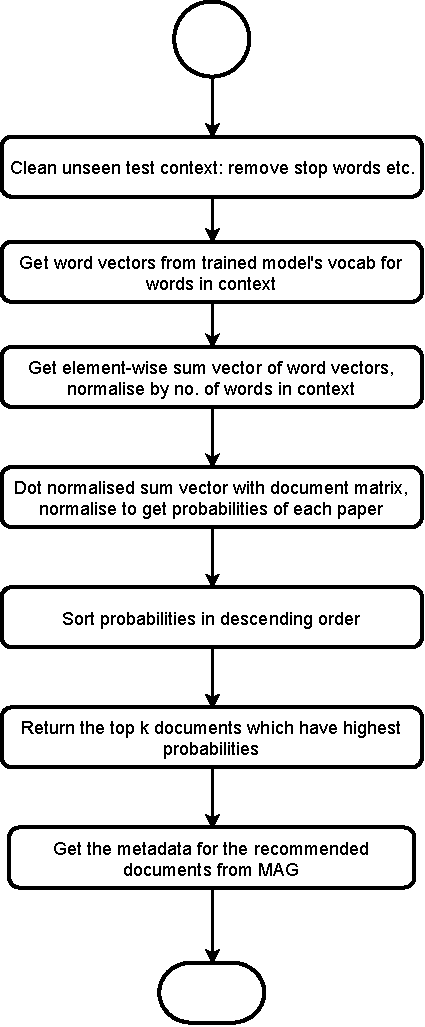
\includegraphics[width=7cm]{figures/Approach/Paper2vectest.pdf}
  \caption{Flowchart: Paper2Vec prediction}
  \label{fig:p2vtest}
\end{figure}
\section{Dual embeddings for hyper-documents: Hyperdoc2vec}
\subsection{Training process}
The Hyperdoc2Vec approach explained in Han et al.~\cite{ShiSZZH18} is a citation recommendation approach which produces two sets of vectors for each paper: IN vectors and OUT vectors (called syn0 and syn1/syn1neg respectively in the popular gensim package). The idea of using dual word embeddings originally comes from \cite{NalisnickMCC16}, in which it is claimed that two vectors work better than one for a variety of tasks. 

Figure~\ref{fig:hd2v} shows the framework for training Hyperdoc2Vec.
Each paper is called a hyper-document in \cite{ShiSZZH18}, as it contains content words as well as annotations (citation markers) which link to other papers. As one of the purposes of the original Hyperdoc2Vec paper is to recommend papers which have not been cited before, it would seem to be a good option to use in the final hybrid algorithm. 
\begin{figure}
\centering
 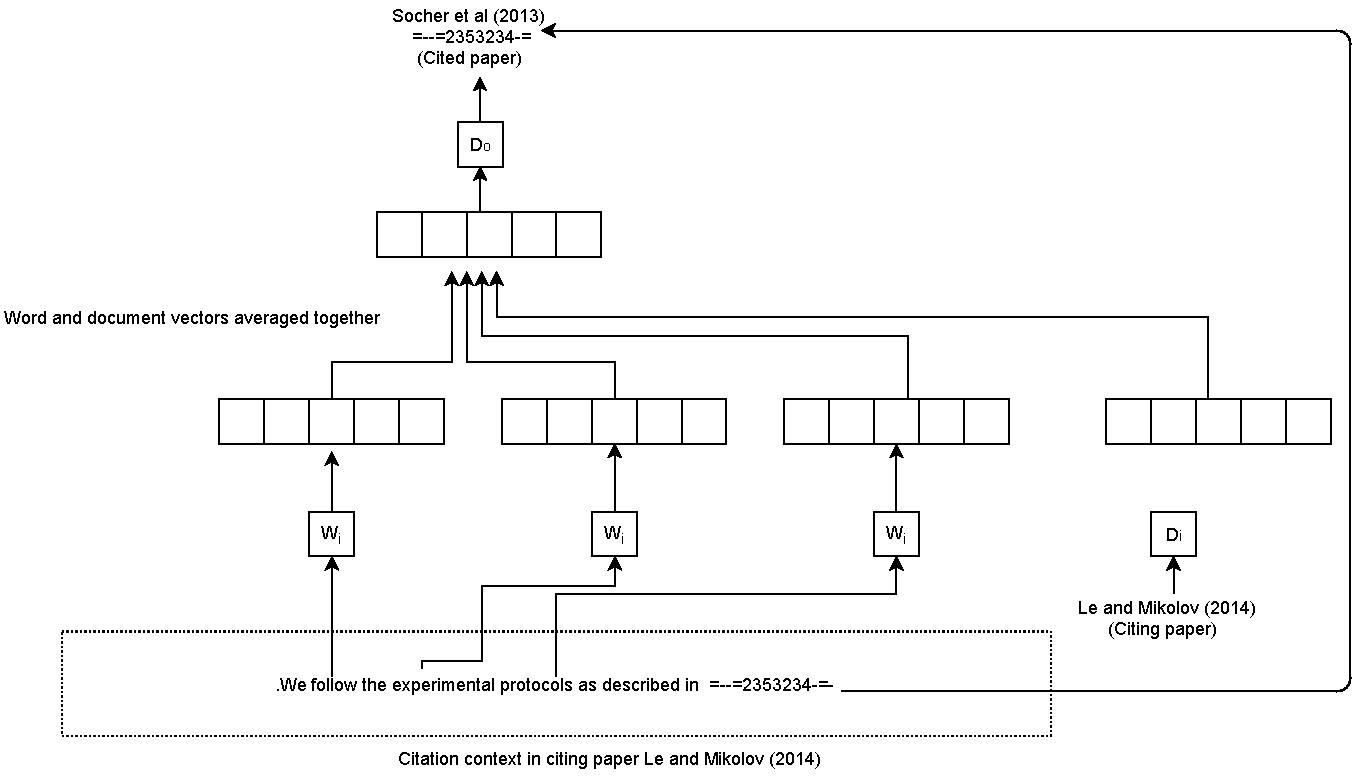
\includegraphics[keepaspectratio, width=13cm]{figures/Approach/hd2v.pdf}
  \caption{Framework for the Hyperdoc2Vec~\cite{ShiSZZH18} model}
  \label{fig:hd2v}
\end{figure}

Before we describe the theory behind the training process, it might be worth mentioning the preprocessing done before training. Like in Paper2Vec, we make words lower-case, remove stop words, expand contractions and remove extra white spaces from the files created in Chapter 4. Appendix~\ref{chap:preprocessing} shows the stop words removed, and explains the preprocessing step in detail.

The entire training process based on~\cite{ShiSZZH18} is shown in the form of a flowchart in Figure~\ref{fig:hd2vtraining}.
In the Hyperdoc2vec approach, for a paper 'P', the IN document vector ($d^I$) represents P playing the role of a source (citing) document. The OUT document vector ($d^O$) represents P playing the role of a target (cited) document. Essentially, this means that the algorithm is both content-aware and context-aware. Both the content of P and the contexts of the papers which cite P play a role in P's embeddings. 

This can be contrasted with the regular Doc2Vec (pv-dm) algorithm described in Section 5.1.1, in which only the IN vectors are generally used. pv-dm is not context-aware, the OUT vectors play no role. 
\begin{figure}
\centering
 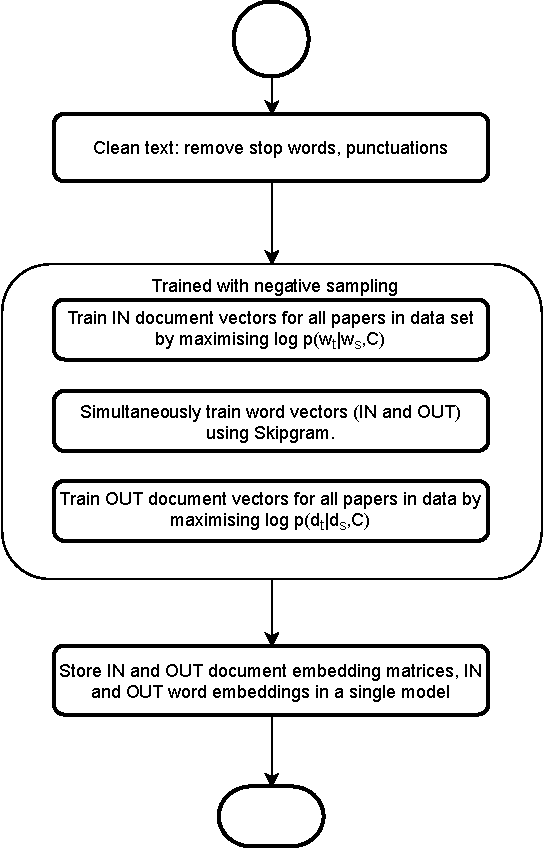
\includegraphics[keepaspectratio, width=8cm]{figures/Approach/hd2vtrainflowchart.pdf}
  \caption{Flowchart: Hyperdoc2vec~\cite{ShiSZZH18} training process}
  \label{fig:hd2vtraining}
\end{figure}
pv-dm maximises $\sum\limits_{w_i, w_j \in c_1}^{|C_1|} log P(w_j|{w_i, d_k})$, the probability of a word given the neighbouring words and the document vector. 

Hyperdoc2vec maximises 2 separate probabilities. Consider the set of all contexts $C={(d_s, C, d_t)}$. The following log probability which models the contexts' impact on the embeddings is the first probability that is maximised: 
\begin{equation}
    \underset{D^I, D^O, W^I}{\max}\; \frac{1}{|C|} \; \sum\limits_{(d_s,C,d_t) \in C}\: log P(d_t|d_s, C)
\end{equation} 
where $D_I$, $D_O$ and $W_I$ are the set of all IN and OUT document vectors, and word vectors respectively. 
\begin{table}
\centering
\caption{Common Hyperparameters across data sets Hyperdoc2Vec}
\label{tab:hd2vhyperparams}
\begin{footnotesize}
\begin{tabular}{ll@{}c}
\toprule
Hyperparameter & Value \\
\midrule
Learning rate &  0.025 \\
Number of training iterations & 100 \\
Half-context window size & 20 \\
Subsampling rate (negative sampling) &  0.001 \\
Vector size & 300 (but 100 for ACL-MAG) \\
\bottomrule
\end{tabular}
\end{footnotesize}
\end{table}
The probability that a cited document $d_t$ is cited in a context C of a citing paper $d_s$ is modelled by averaging the IN word vectors of the words in the context.
\begin{equation}
    x = \frac{1}{1+|C|} (d_S^I + \sum\limits_{w\in C} w^I)
\end{equation}
Finally, this average of vectors is combined with the OUT document vectors to implement a multi-class softmax classifier (as in Section 5.1).
\begin{equation}
    P(d_t|d_s, C) = \frac{exp(x^T d+t^O)}{\sum\limits_{d\in D} exp(x^Td^O)}
\end{equation}
The contents' impact on the papers' embeddings is also modelled. This is done by predicting the OUT word vector of each word from the neighbouring word and the document vector, as in pv-dm. The equation for a source document $d_s$ is: 
\begin{equation}
    P(w_j|{w_i, d_s}) = \frac{exp(w_j^Tw_i + w_j^td_s)}{\sum_{t=1}^{C_1}{exp(w_t^Tw_i + w_t^Td_s)}}
\end{equation}
Here, $w_j$ is the 'current' word vector, and the word vectors of the other words in the same context are represented by $w_i$.
The following equation is maximised: 
\begin{equation}
    \sum\limits_{w_i, w_j \in c_1}^{|C_1|} log P(w_j|{w_i, d_k})
\end{equation}
\begin{figure}
\centering
 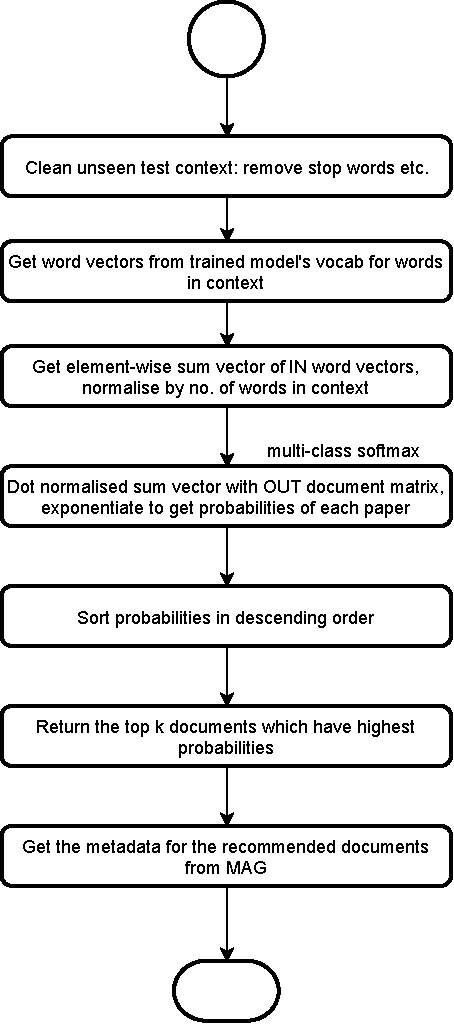
\includegraphics[width=7cm]{figures/Approach/hd2vOUT.pdf}
  \caption{Flowchart: Prediction using Hyperdoc2vec OUT document vectors and IN word vectors of context (hd2vOUT)}
  \label{fig:hd2vOUT}
\end{figure}
The main hyperparameters used are the vector size and the size of the context window. The hyperparameter for calculating the size of the context window is the 'half-context window'. The half-context window used for all the data sets is 20 in this thesis. This means that the citation context is made up of 40 words while training the algorithm. Experiments showed that this worked well as the average citation context length seemed to be around 40. The vector sizes are kept constant for all the data sets except the small ACL-MAG data set. The hyperparameters used are shown in Table~\ref{tab:hd2vhyperparams}.\\
In this thesis, we divide the Hyperdoc2Vec algorithm into two for the testing and evaluation phases based on which vectors are used. When only the OUT document vectors are used, we call the algorithm hd2vOUT. When both IN and OUT document vectors are used, we call the algorithm hd2vINOUT.

\subsection{Testing process}
There are 4 possible combinations of document and word vectors which we can choose from. The first option is to use a multi-class softmax classifier after taking a dot product of the OUT document matrix (made up of OUT document vectors) and the average of the IN vectors of the context words. This is shown in equation (8). The multi-class softmax classifier returns a probability for each paper in the training corpus. These probabilities are sorted and the top n recommendations are returned. This version of the algorithm is called hd2vOUT and the complete process is sketched out as a flowchart in Figure~\ref{fig:hd2vOUT}.

The other three combinations (OUT document vectors and OUT word vectors, IN document vectors and IN word vectors, IN document vectors and OUT word vectors) do not work as well as the first option. 

Another thing we can do is to use the embeddings based on both the contents and the contexts and feed this to another multi-class softmax classifier. This is done by taking the dot product the averaged IN word vectors of the context with the OUT document matrix, taking the dot product of the averaged OUT word vectors of the context and the IN document matrix, and adding the two vectors together. A final exponentiation completes the process.
As before, this multi-class softmax classifier also returns a probability for each paper in the training corpus. These probabilities are sorted and the top n recommendations are returned. This version of the algorithm is called hd2vINOUT and the process is shown in Figure~\ref{fig:hd2vINOUT}.
\begin{figure}
\centering
 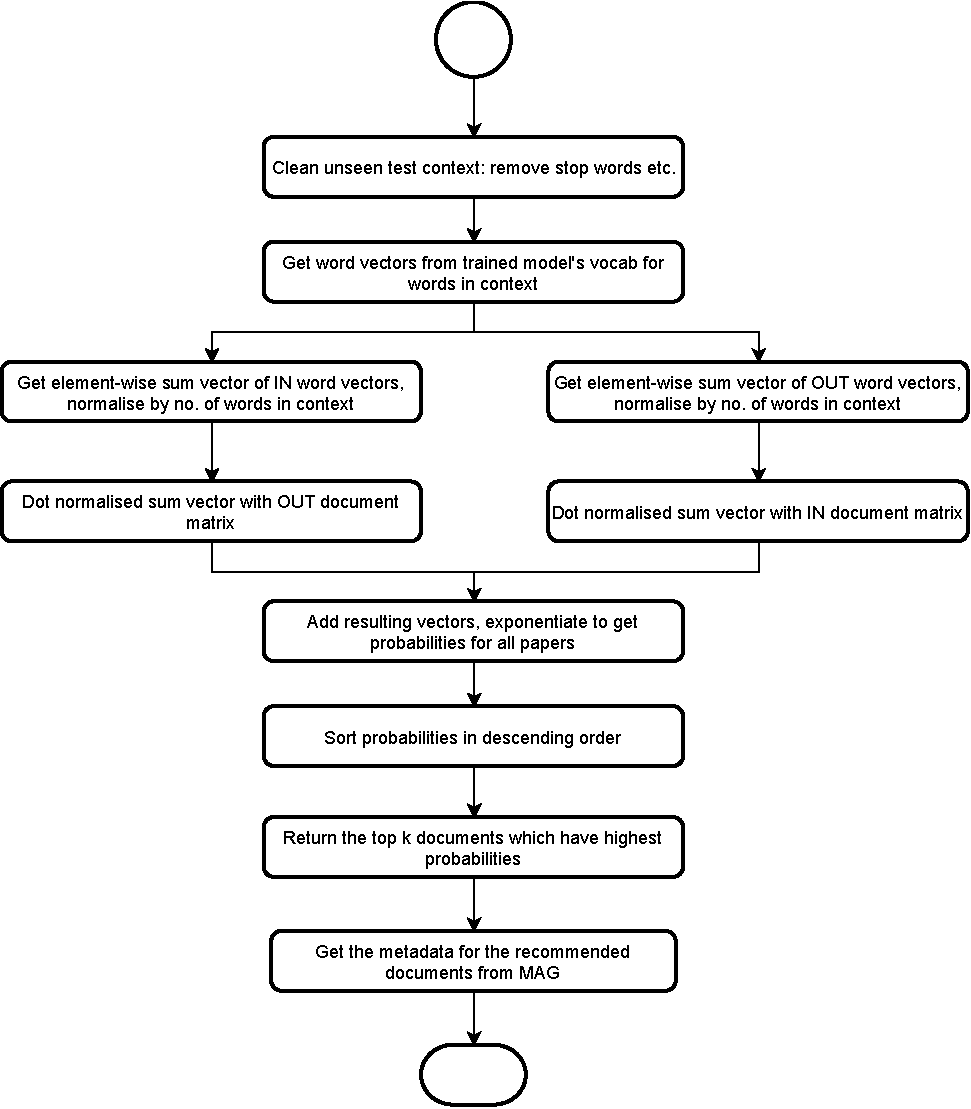
\includegraphics[width=15cm,height=17cm]{figures/Approach/hd2vINOUT.pdf}
  \caption{Flowchart: Prediction using Hyperdoc2vec OUT document vectors and IN word vectors of context, IN document vectors and OUT word vectors (hd2vINOUT)}
  \label{fig:hd2vINOUT}
\end{figure}

As we will see in the next chapter (chapter 6), using the OUT document vectors with the IN word vectors is the method that works best of all. Using both the IN and OUT document vectors doesn't work as well in practice.
\section{Topic Modelling and Information Retrieval algorithms}
\subsection{Similar topic models using LDA}
The idea behind using the Latent Dirichlet Allocation (LDA) \cite{BleiNJ03} for citation recommendation is to recommend papers whose content maps to a similar set of topics as those of the test citation context. The flowchart for the LDA training process is given in Figure~\ref{fig:ldatrainingflowchart}.
\begin{figure}[h]
\centering
     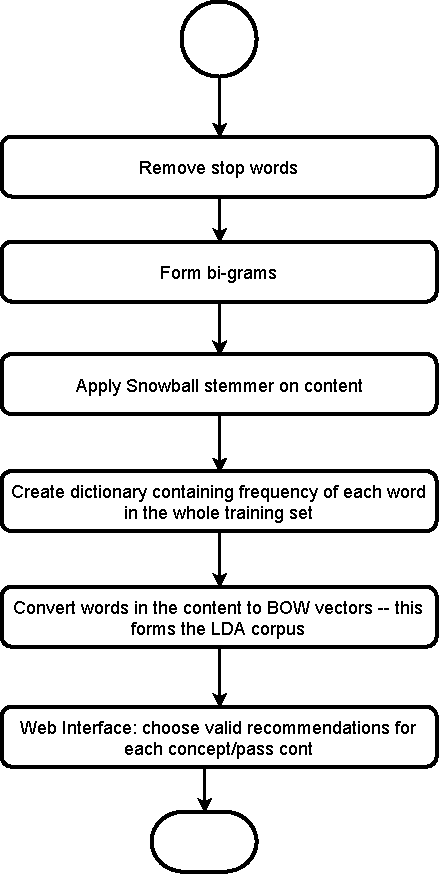
\includegraphics[width=6cm]{figures/Approach/LDAtrainingflowchart.pdf}
  \caption{Flowchart: LDA Training process}
  \label{fig:ldatrainingflowchart}
\end{figure}
\begin{figure}
 \centering
 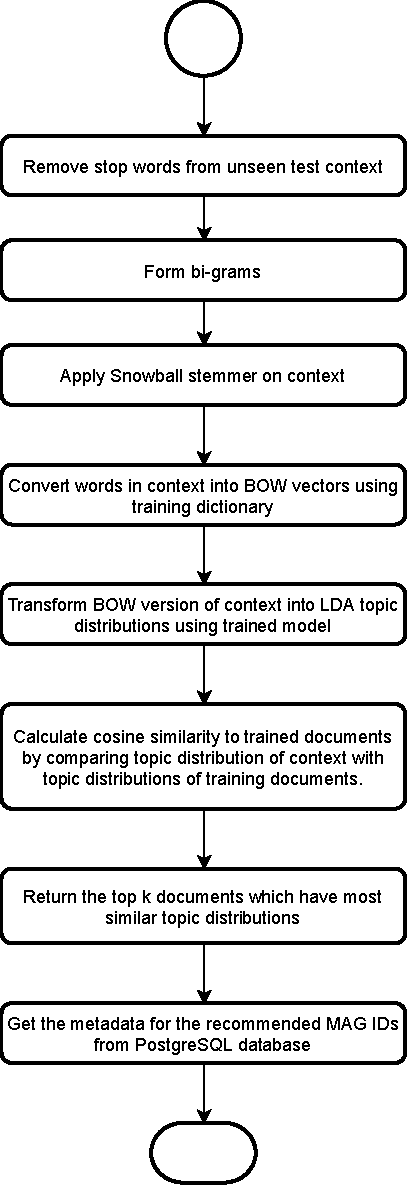
\includegraphics[width=6cm]{figures/Approach/LDAtestingFlowchart.pdf}
  \caption{Flowchart: LDA Prediction}
  \label{fig:ldapredictflowchart}
\end{figure}
The Gensim package is used for getting the topic models. It was found during testing that the MALLET implementation of LDA \footnote{http://mallet.cs.umass.edu/} produced higher-quality topic models than the normal Gensim version of LDA. The difference between MALLET and the normal Gensim LDA is that MALLET uses Gibbs sampling while the normal Gensim LDA uses a Variational Bayes sampling method. While Gibbs sampling is more precise, MALLET takes an inordinate and impractical amount of time for prediction. Therefore, it was decided to use only the normal LDA during evaluation. However, the LDA Mallet is evaluated in Chapter 6 for the smallest ACL-MAG data set, and it performs slightly better than the normal LDA (but much worse than most of the other non-LDA algorithms).\\
The first step to use LDA for citation recommendation is the preprocessing step. This is much more complex than the preprocessing done for the embedding algorithms. Stop words are removed first, and then bi-grams are created. This is then followed by a stemming process using the Snowball stemmer. 
Once this is done, the dictionary and the corpus for LDA can be built. The dictionary maps words to their frequencies over the whole training set. The corpus contains bag-of-words representations of all the documents. The topic model is created from the dictionary and corpus. The number of topics is a hyperparameter which has to be chosen. In this thesis, experiments were done with between 100 and 500 topics and the perplexity was calculated. The number of topics used finally was 300 for all the large data sets and 200 for the small ACL-MAG data set.

The same preprocessing is performed while doing the prediction and evaluation on a citation context, and the words in the context are mapped to topics. After converting this context into a bag of words, we compare the topics of the context with the topics of all the papers in the training set using cosine similarity. The similarities are sorted in descending order, and the top n similar papers are recommended.
The flowchart for the LDA testing process is given in Figure~\ref{fig:ldapredictflowchart}.
\subsection{BM25}
The famous Okapi BM25 algorithm is a bag-of-words algorithm used in citation recommendation approaches, sometimes as a pre-filter and sometimes as a simple baseline. BM25 ranks returned documents based on the query terms appearing in each document. However, the specific position of the query terms makes no difference to the ranking function. For example, if the query terms are 'information', 'retrieval' and 'technique', it will assign the same score to two different documents which have the three words the same number of times, but in different order. 

\begin{figure}
\centering
 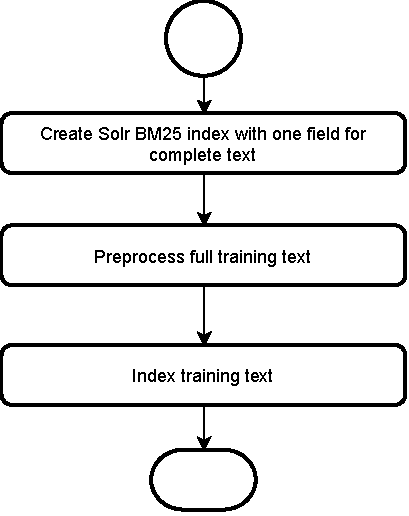
\includegraphics[width=6cm]{figures/Approach/bm25trainingflowchart.pdf}
  \caption{Flowchart: Solr BM25 Training process}
  \label{fig:bm25trainingflowchart}
\end{figure}
To implement BM25, the open-source indexing engine Apache Solr (which runs on Apache Lucene) is used. After preprocessing, the entire content of the document, whether it is from MAG or the other data sets, is indexed in Solr in a single field. 
The training process for BM25 is given in Figure~\ref{fig:bm25trainingflowchart}.
\begin{figure}[h]
 \centering
 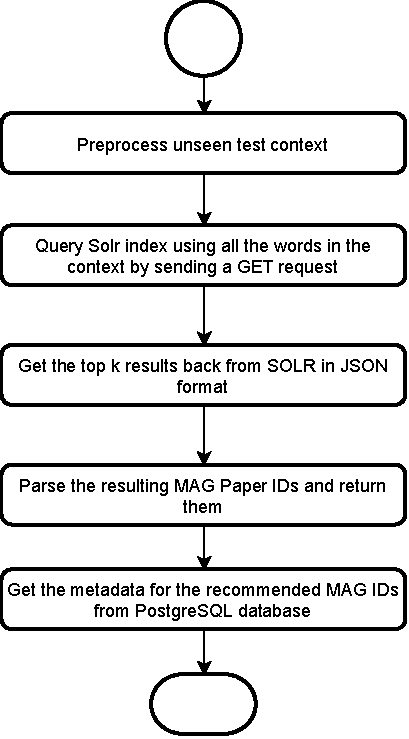
\includegraphics[width=6cm]{figures/Approach/bm25testflowchart.pdf}
  \caption{Flowchart: BM25 Prediction}
  \label{fig:bm25predictflowchart}
\end{figure}
While testing, the queries are constructed as a simple query consisting of all the terms in the preprocessed citation context. A GET request is sent to Solr with the words as parameters, and the top n results are returned. The similarity used while comparing the BM25 vectors is, like in the case of LDA, cosine similarity. 
The flowchart for the BM25 prediction process is given in Figure~\ref{fig:bm25predictflowchart}.\\
The MAG-Cited data set described in Section 4.2.6 is also indexed in the same way as Figure~\ref{fig:bm25trainingflowchart} so that it can be used in the improved hybrid algorithm in Section 5.5 and the case study in Section 6.2.4. The testing process for the MAG-Cited data set is also exactly the same as described in Figure~\ref{fig:bm25predictflowchart}.

\section{Semi-genetic Hybrid recommeder for Citation recommendation}
Recommendations from different recommender systems can be combined in many ways. It can be as simple as giving scores to each recommender system's recommendations based on ranks, and adding the scores for items which have been recommended by both recommender systems. However, there are a number of questions which can be raised in this case. Is an item that is ranked 50 and 80 by two recommender systems a better candidate than another item which has been ranked 5 and 240? How should we score items which have been ranked highly (say, 2) by one recommender system, but which haven't been returned at all by the second recommender system. These are questions with no obvious answers.

An interesting option would be to use a weighted hybrid algorithm which combines recommendations stochastically.  Mueller~\cite{Mueller17} describes one such algorithm which can be used to construct a 'semi-genetic' hybrid recommender. The algorithm is called 'semi-genetic' because it uses only some of the steps of the genetic algorithm explained in Chapter 3. The cross-over and mutation steps of genetic algorithms are skipped. In addition, the semi-genetic algorithm has only one iteration, unlike most genetic algorithms. 
In this thesis, we implement this algorithm to build a semi-genetric hybrid citation recommendation system. A flowchart of our hybrid citation recommendation system is shown in Figure~\ref{fig:hybridflowchart}.

The recommendations from the best individual algorithms described previously are fed into this semi-genetic hybridisation algorithm. Experiments conducted across data sets (the evaluations results are described in Chapter 6) indicate that some of the algorithms do a lot better than others. Using all the algorithms as part of the hybrid recommender did not increase its recall. For this reason, our hybridisation algorithm combines recommendations from only two individual recommenders -- the BM25 recommender, and the Hyperdoc2vec recommeder with OUT document vectors (hd2vOUT). Using only the OUT vectors (along with the IN word vectors of the words in the context) works almost twice as well as using both the IN and OUT document vectors, as shown in Chapter 6. 

The steps of the semi-genetic hybridisation algorithm for combining BM25 and hd2vOUT recommendations are given below. The process runs for only one iteration, unlike most genetic algorithms.

\textbf{Step 1.} Initialise population: select a set of items from all possible 'chromosomes', i.e. from the recommendation lists of both component algorithms. In this step, we get the top 500 recommendations from BM25 and the top 500 recommendations from hd2vOUT, and concatenate them.

\textbf{Step 2.} Evaluate fitness scores: The reciprocal rank is assigned as the fitness score for the recommendations from each of the algorithms. Using the reciprocal rank is a fair proxy for the fitness score -- if an algorithm ranks a paper highly, it indicates that it gives the paper a high score. For example, if paper A has been ranked 1 by BM25, its fitness score for BM25 is 1/1. If the same paper has been ranked 200 by hd2vOUT, its fitness score for hd2vOUT is 1/200. Let's say Paper B has been ranked 10 by BM25. Then its fitness score for BM25 is 1/10. If Paper B hasn't been returned by hd2vOUT, there is no fitness score associated with it for hd2vOUT. Note that the two component algorithms have been given equal weights in this step.

At this stage, we have an array of 1000 recommendations, 500 from hd2vOUT and 500 from BM25. Each of the recommendations is associated with a fitness score (reciprocal rank). If a paper has been recommended by both algorithms, it will have two scores associated with it.

\textbf{Step 3.} Convert the scores into probabilities. This is done by dividing each score by the sum of all the scores.
\begin{figure}
 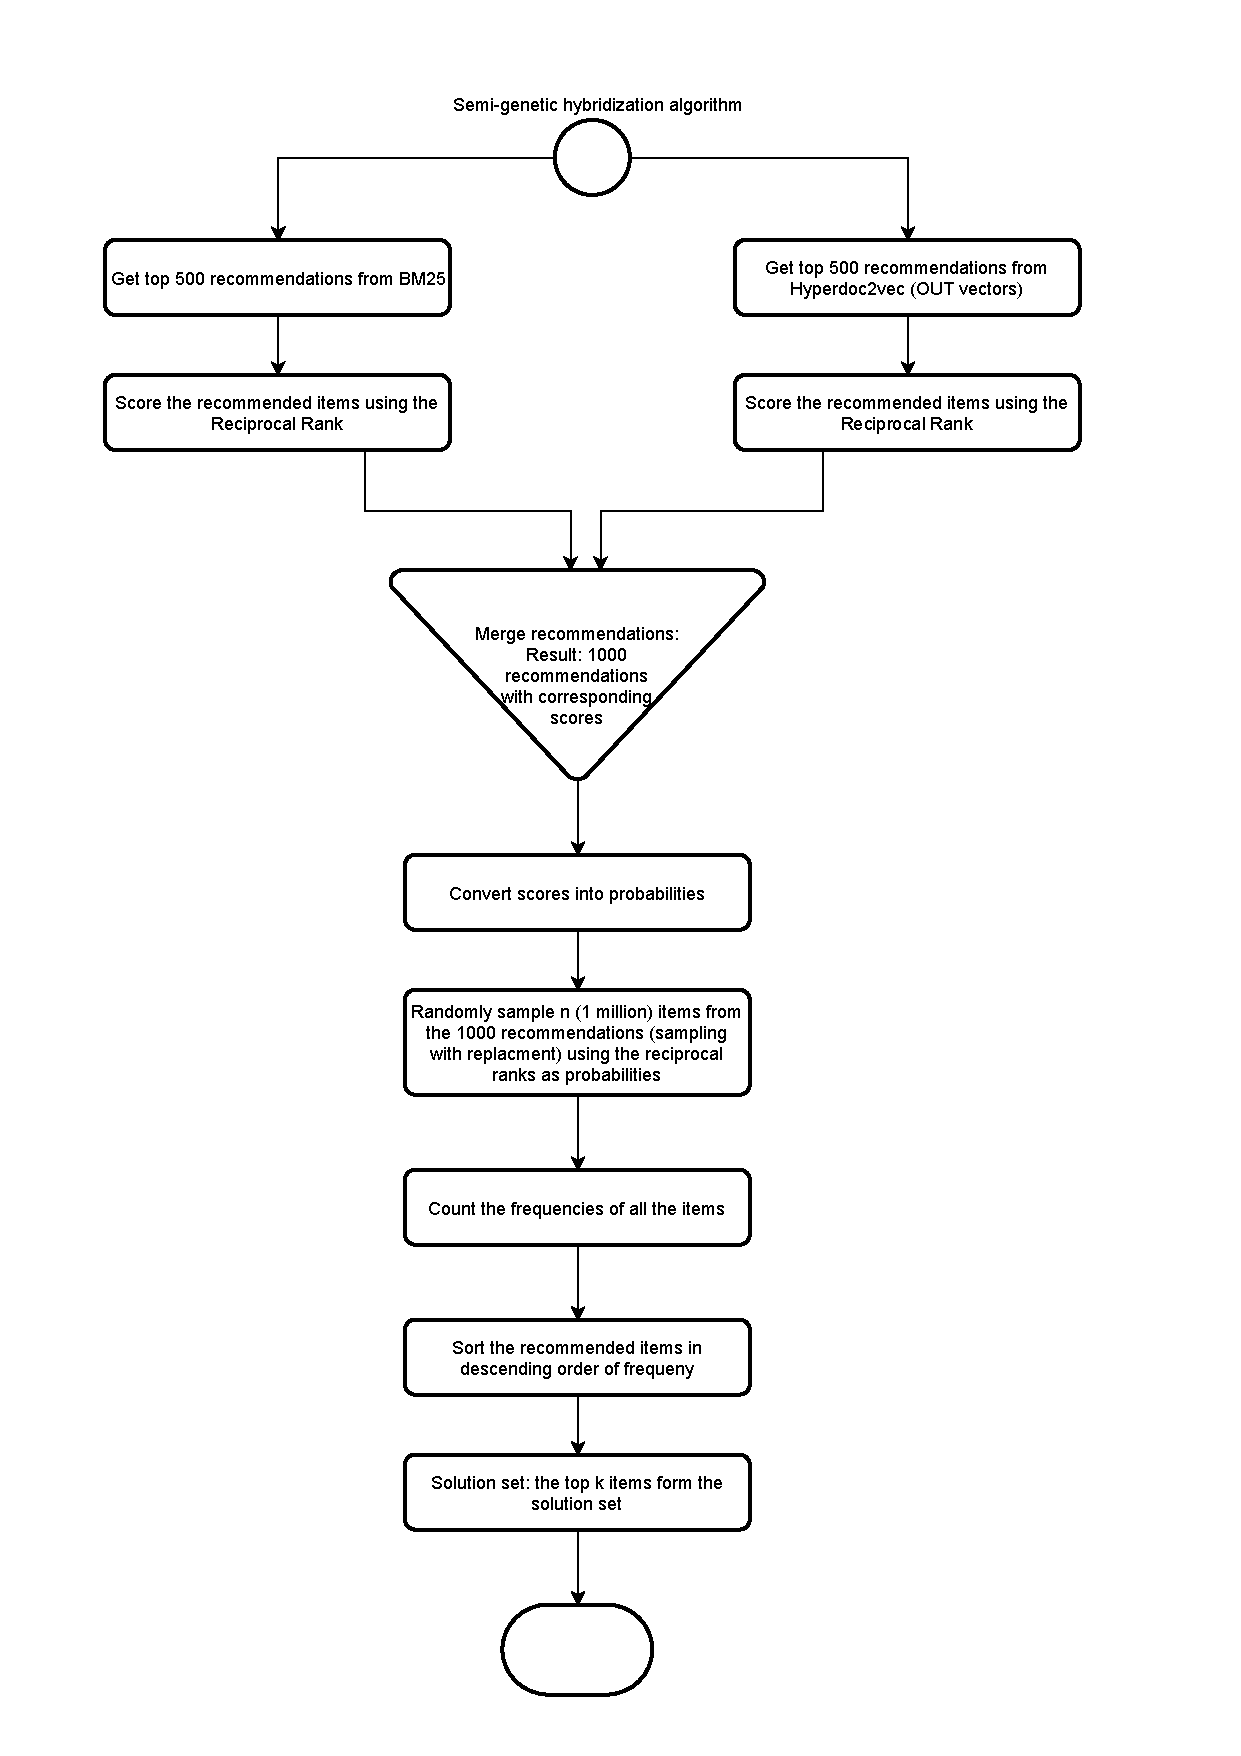
\includegraphics[keepaspectratio, width=14cm]{figures/Approach/Hybridflowchart.pdf}
  \caption{Flowchart: semi-genetic hybridisation algorithm for citation recommendation}
  \label{fig:hybridflowchart}
\end{figure}

\textbf{Step 4.} Selection: we randomly draw n (n = 1 million) samples with replacement from the array of 1000 recommendations. The idea is that papers which have higher ranks in either of the lists will have a higher probability of being drawn in the random sample. Papers which have been recommended by both the component recommenders have two distinct probabilities of being drawn. A paper which has been ranked highly by both algorithms (say 1 and 3) will have a very high probability of being drawn in the random sample.

As the random sample is made with replacement, the best recommendations from both the algorithms combined will be recommended the most number of times. This is a stochastic process, and we expect the random draws to depend on two factors: (i) its probability of being drawn in either algorithm -- the higher the better, (ii) the presence of a paper in both recommendation lists -- however, the individual ranks in each of the lists matter immensely. So, a paper which has been ranked 400 and 500 by the two algorithms may get picked a lot less than a paper which is not present in one algorithm's recommendation list, but has been ranked 2 by the other algorithm.

\textbf{Step 5.} Count the number of times each of the papers is drawn. 

\textbf{Step 6.} Sort the recommendations in descending order of frequencies. 

\textbf{Step 7.} Solution set: at this stage, the sorted array of recommendations will have at most 1000 papers, but usually less than 1000 papers (as the two component algorithms will usually recommend at least some common papers). To get the final solution set, we return the top k recommendation from the sorted array of recommendations.
\section{Hybrid23: Improved Hybrid algorithm based on 2 MAG data sets and 3 components}
While the hybrid algorithm explained in Section 5.4 works better than its individual components, its performance can be improved further by using two data sets. 

The data sets we use for this algorithm are the regular MAG data set described in Section 4.2.2 and the MAG-Cited data set described in Section 4.2.6. The MAG-Cited data set, like the normal MAG data set, contains pseudo full-text for the content of each paper. However, the citation contexts in a paper's pseudo full-text are from papers which cite it. 

The BM25 algorithm performs much better in an offline evaluation on the MAG-Cited data set compared to the MAG data set, as we show in a case study in Section 6.2.4. This is due to the fact that citation contexts tend to describe the cited papers better than the citing papers. Therefore, the text-matching based BM25 algorithm works better when the citation contexts from a citing paper are present in a cited paper's content. 
\begin{figure}
 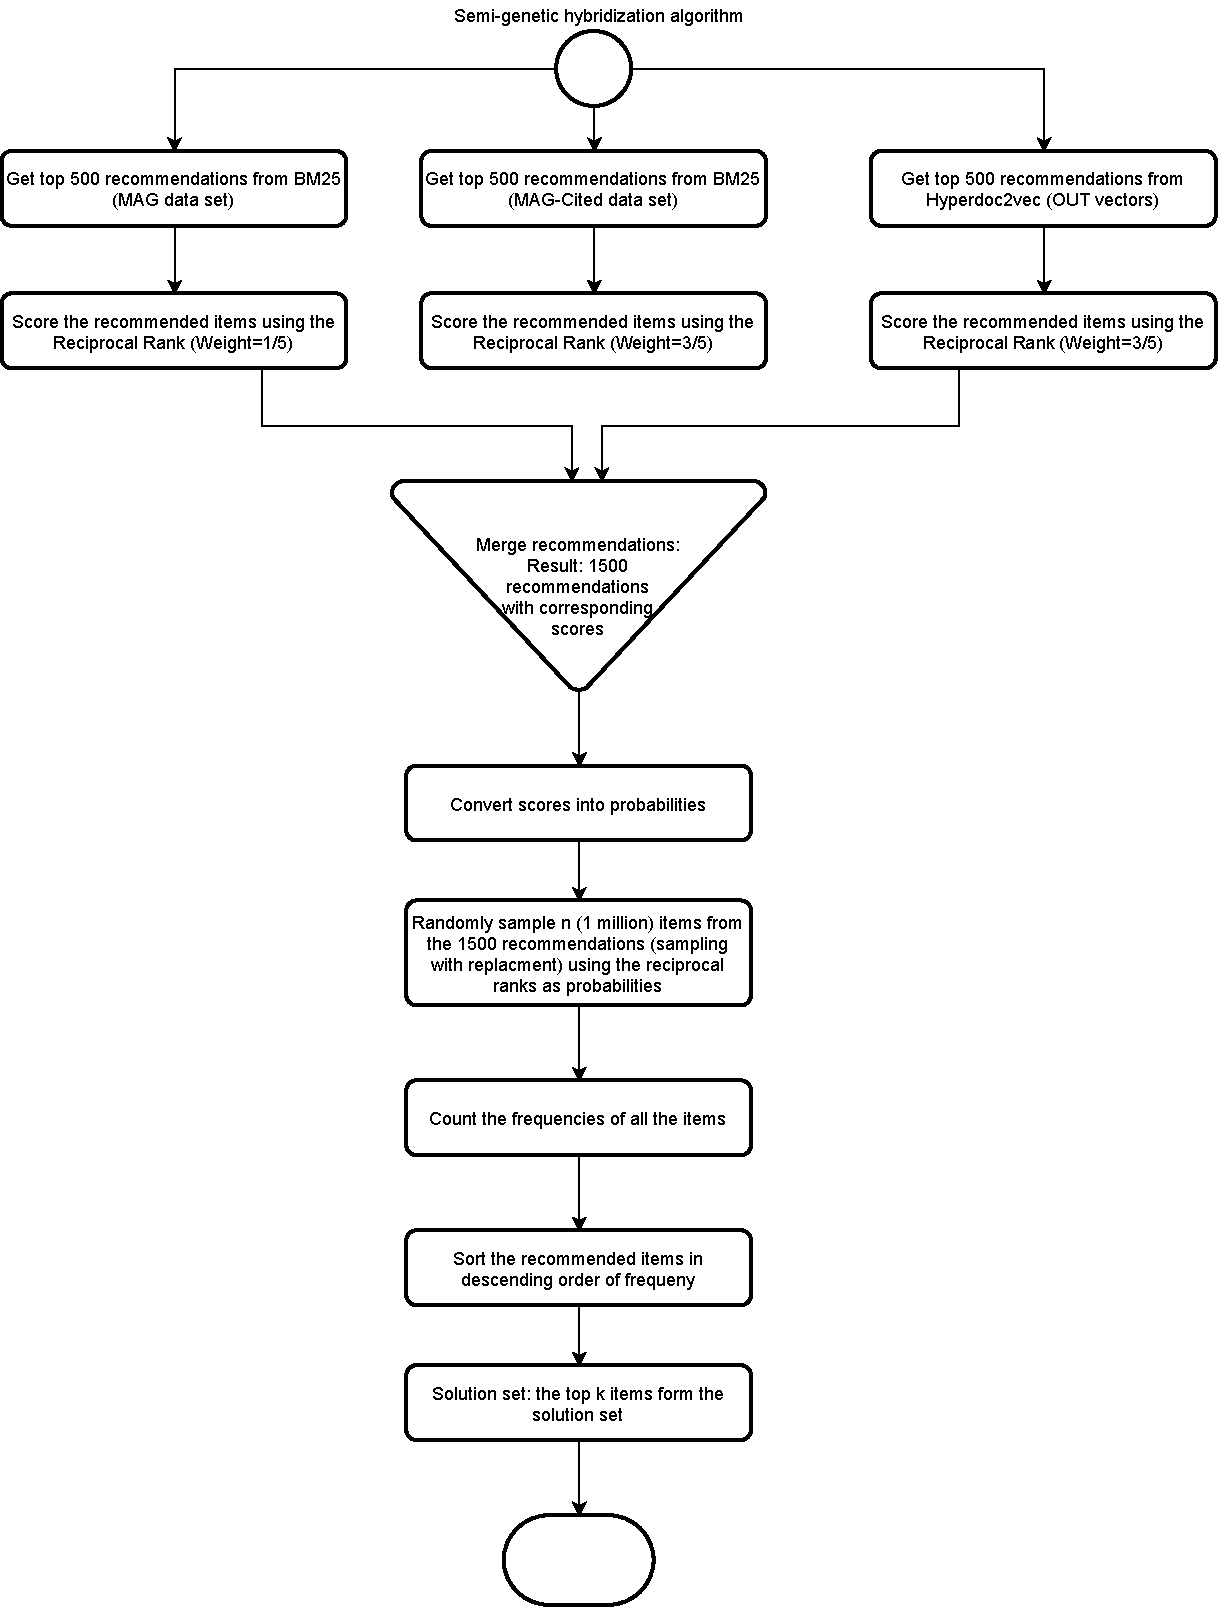
\includegraphics[keepaspectratio, width=14cm]{figures/Approach/hybridv2flowchart.pdf}
  \caption{Flowchart: Hybrid23 -- improved semi-genetic hybridisation algorithm which uses two MAG data sets and three components}
  \label{fig:hybridv2flowchart}
\end{figure}
The improved hybrid recommender system uses the above two data sets and contains three components. It is therefore called \textbf{Hybrid23}. Its three components are:
\begin{enumerate}
    \item hd2vOUT trained on the MAG data set
    \item BM25 trained on the MAG data set
    \item BM25 trained on the MAG-Cited data set
\end{enumerate}
A flowchart for the Hybrid23 is shown in Figure~\ref{fig:hybridv2flowchart}.
The algorithm is almost the same as the one in Section 5.4, but there are changes in Steps 1 and 2 due to the fact that there are three components. The steps are explained below.\\
\textbf{Step 1.} Initialise population: select a set of items from all possible 'chromosomes', i.e. from the recommendation lists of the \textit{three} component algorithms. In this step, we get the top 500 recommendations from BM25 (MAG), hd2vOUT (MAG), BM25 (MAG-Cited) and concatenate them. At the end of this step, we have a list of 1500 recommendations.\\
\textbf{Step 2.} Evaluate fitness scores: The hybrid algorithm in Section 5.4 gave equal weights to the two component algorithms. But now, we have three component algorithms in which one (BM25 for MAG-Cited) works much better than the others. So while the reciprocal rank is still assigned as the fitness score for the recommendations from each of the algorithms, it is weighted differently. The reciprocal ranks for the recommendations from the BM25 algorithm for MAG-Cited are multiplied by a weight of 3/5 (60\%), while the reciprocal ranks of the recommendations from the other two algorithms (BM25 for MAG and hd2vOUT) are multiplied by a weight of 1/5 (20\%) each. 
E.g.: the fitness scores of the second-ranked recommendation from the BM25 (MAG-Cited) component is 3/10, while the fitness scores for the second-ranked recommendation from the other two components are 1/10 and 1/10 respectively. ran At the end of the step, we have 1500 recommendations with their respective fitness scores.\\
\textbf{Steps 3-7} are exactly the same as the algorithm described in Section 5.4, except for the fact that we now have 1500 recommendations instead of 1000 recommendations. The probabilities of picking recommendations from the BM25 (MAG-Cited) component are much higher.

\section{HybridCite: Running Citation Recommendation System}
An online citation recommendation system is created in which the user is allowed to enter free text and get citation recommendations. 
After the observations made during the process of doing the online and offline evaluation (including the case study in Section 6.2.4), the improved hybrid algorithm (Hybrid23) described in Section 5.5 was chosen as the algorithm to use under the hood in the running system. Additionally, it was decided that the users would be given a few options, which will be described shortly.

\begin{figure}
    \centering
    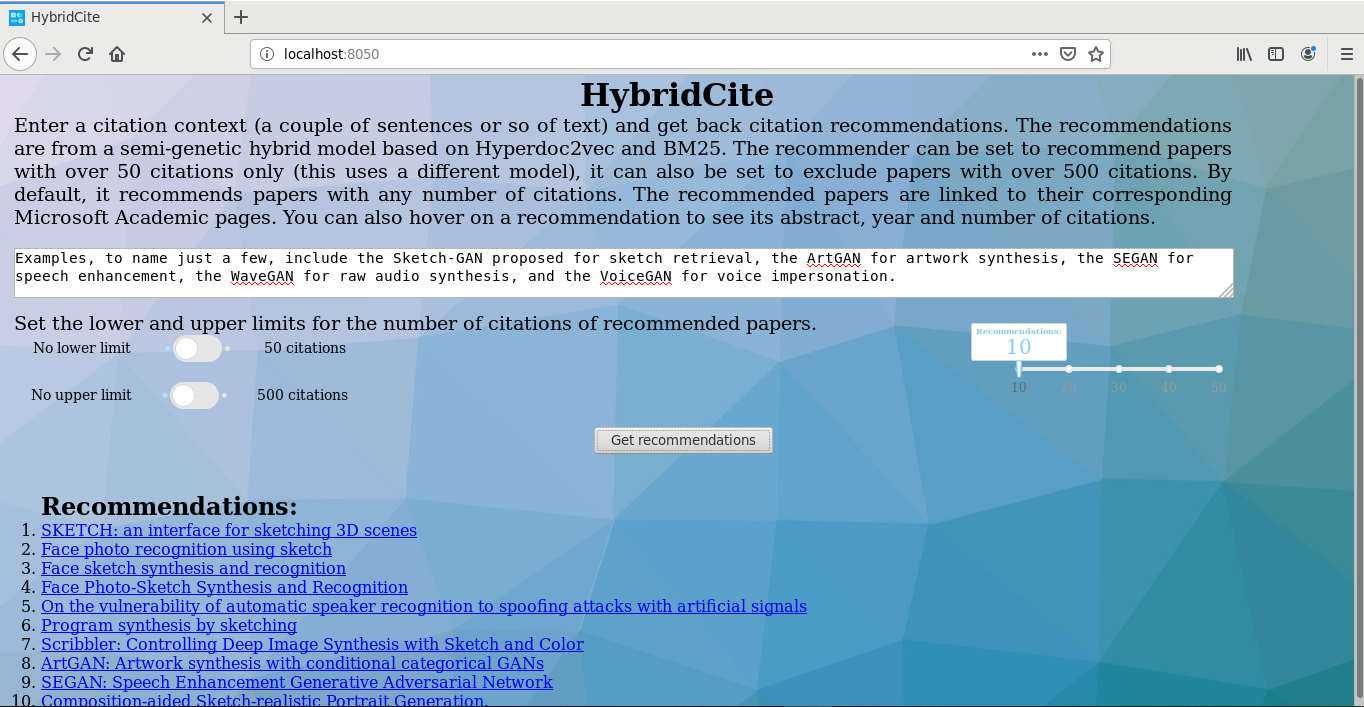
\includegraphics[keepaspectratio, width=13cm]{figures/Approach/recommsystem.PNG}
    \caption{Interface of the citation recommendation system 'HybridCite'}
    \label{fig:hybridcite}
\end{figure}
Two separate models are used in the final recommendation system -- Hybrid23 models trained on the MAG (and MAG-Cited) and MAG50 (and its corresponding reduced version of MAG-Cited) data sets. MAG50 contains only papers which have been cited 50 times or more. The reason for including the MAG50 model is that some users might not want to be recommended papers which haven't been cited much. On the other hand, it is likely that other users might know the popular papers and would want to be recommended more obscure papers. 

The default model used is the one based on the main MAG and MAG-Cited data sets, but users who want to be recommended reasonably well-known papers might want to use the MAG50 model. It is important to note at this stage that the MAG50 model will also miss new papers because they haven't had the time to get 50 citations. 

Another option that is given to the users is to remove very popular papers which have more than 500 citations. It is unlikely that a researcher doing research on word embeddings will want to be recommended the popular Word2Vec paper, or that a person researching uses of SVMs might want to be recommended the original SVM paper. These papers are so popular that most researchers will have heard of them, and the recommendation might not therefore be useful.

Finally, the user can choose to get more than the default 10 recommendations -- he/she can choose to get 20, 30, 40 or 50 recommendations. Each time the number of recommendations is changed, new recommendations are retrieved and the page is dynamically updated. This involves getting fresh recommendations from hd2vOUT and the two BM25 implementations, and combining them again using the hybrid algorithm. It is entirely possible (and probable) that the recommendations in the new list retrieved from the hybrid algorithm might be in a different order to the previous list. The hd2vOUT and BM25 algorithms might return recommendations in slightly different order, and the stochastic hybrid algorithm may select different papers in its result set. So if the user gets 10 recommendations, and later changes the number of recommendations to 20, the papers at the top of the list might be different from the ones at the top of the list when 10 recommendations were retrieved.

The interface of the recommendation system is shown in Figure~\ref{fig:hybridcite}. The recommended papers returned are linked to their corresponding pages on Microsoft Academic. The abstract, published year and the citation count are visible as a tooltip when the user hovers on the link to the recommended paper. These citation counts are as per the values currently in the underlying database and might not match the citation counts on the latest Microsoft Academic page.
    \chapter{Evaluation}\label{chap:evaluation}
Citation recommender systems are arguably more difficult to evaluate than other types of recommender systems. The evaluation depends heavily on the ground truths which are chosen. In this case, the ground truths are the papers \textit{actually cited} by the authors in the test citation contexts. So the task performed during evaluation is the task of re-prediction. 

However, this is a very subjective way of carrying out an evaluation. There is no reason to believe that all the test contexts' authors have cited the correct papers. Not all people who author papers are experienced researchers, so it is possible that they missed other suitable papers which might have been cited in the same place. What this means for the evaluation is that the citation results produced by the algorithms might actually be suitable even though they are not present in the ground truth. For this reason, it is important to conduct an online evaluation (user study) in conjunction with a normal offline evaluation. 

There is also the possibility that the test citation context might not have enough information necessary to make the prediction. It might be the case that the correct paper to cite becomes clear only after reading adjacent paragraphs in the paper. MAG, in particular, has a lot of citation contexts from which it is not possible to recommend any paper. This is a common problem which will bring down the metric scores, but that is the nature of the citation recommendation problem. 

The following section (6.1) gives a short description of the evaluation metrics used. Sections 6.2 and 6.3 describe the offline and online evaluation respectively.

\section{Evaluation Metrics}

Before calculating the metrics, the recommendations are binarized. For three of the metrics, this step assigns a '1' for a relevant recommendation (a paper in the ground truth) and a '0' for a recommendation which is not in the ground truth. 

The NDCG metric which will be described shortly assigns different relevance values to different relevant documents. This applies only in the case of Arxiv-MAG where we have considered one primary recommendation and other secondary recommendations. Here, a '2' is assigned for the primary recommendation, '1' is assinged for a secondary recommendations and '0' is assigned to recommended papers which are not part of the ground truth. In other words, primary recommendations are twice as important as secondary recommendations while calculating the NDCG.

It is important to note that the NDCG is not very useful when used with the other data sets which don't have graded ranks (such as MAG). While it is still reported for all the data sets, it is not a metric which we pay a lot of attention to.

In the following definitions, the word 'query' refers to a test set citation context for which recommendations are retrieved.

\textbf{Precision@k}: The precision@k gives the percentage of relevant documents in the top k recommendations for a single query. \\
Example: the binarized array [1, 0, 0, 1, 0] has precision@3=1/3, precision@5 = 2/5

\textbf{Average Precision (AP)}: Let $K_1,K_2,...,K_R$ be the ranks of each relevant document. The average precision for a query (test context) gives the average of precision@k values for $K_1,K_2,...,K_R$.\\
Example: the binarized array [1, 0, 0, 1, 0] has an average precision of $\frac{(1/1 + 2/4)}{2}$.

\textbf{Mean Average Precision (MAP)}: This is the first of the metrics that is reported for our data sets. The mean average precision is simply the mean of the average precision values over multiple queries (test set contexts).
Let the average precisions of the recommendations for all the n test set contexts are $AP_1, AP_2, AP3, ..., AP_n$. Then, 
\begin{equation*}
    MAP = \frac{\sum\limits_{i=1}^n AP_i}{n}
\end{equation*}
\textbf{Recall@k}:
Recall is a measure which gives the percentage of true positives found in the first k recommendations for a single query. 

While average precision averaged over queries is called mean average precision, Recall@k when averaged over queries, is still called Recall@k. This is a bit of a misnomer, but the term 'Recall@k' actually refers to the \textit{Average Recall@k} while evaluating recommender systems.
So in this thesis, Recall@k gives the average recall over all n test set contexts.
\begin{equation*}
    Recall = \frac{\sum\limits_{i=1}^n R_i}{n}
\end{equation*}
where R is the recall for a single test set context.
Example: Let there be 3 relevant items in the ground truth and two queries in the test set.
The binarized array [0,0,1,0,0] has a R@5 of 1/3. The binarized array [1,0,0,1,0] has a R@5 of 2/3. So the final Recall@5 = $\frac{(1/3 + 2/3)}{2}$

\textbf{Reciprocal Rank (RR)}:
The reciprocal rank is simply the reciprocal of the rank of a relevant item. 

\textbf{Mean Reciprocal Rank (MRR)}:
The MRR is obtained by averaging the reciprocal ranks over all queries. It is a metric which is most often used when there is only one relevant item. 
As the test sets in this thesis \textit{generally} have only one relevant item in the ground truth list, this is a useful metric. In cases where there is more than one relevant item in the ground truth list, only the  rank of the \textit{highest-ranked relvant item} is considered. 

Example: the MRR of the binarized arrays [0,1,0,1,0] and [0,0,1,0,0] is $\frac{(1/2 + 1/3)}{2}$. Only the reciprocal rank of the highest-ranked relevant item is used in the MRR calculation.

\textbf{Discounted Cumulative Gain (DCG@k)}:
This is a metric which assumes that relevant documents have different degrees of relevance. In this thesis, this only applies to the Arxiv-MAG data set, in which the primary recommendation gets a value of '2', and the secondary recommendations (if present) get a value of '1'. 

The 'gain' obtained from secondary recommendations is less (it is discounted) than the gain obtained from a primary recommendation.
There are different discounts used in DCG calculations. In this thesis, a discount of $1/log_2 i$ is applied (where i is the position of the rank).
The discounts applied are therefore [1.0, 1.0, 0.6309, 0.5, 0.4307, ...]. 

Let $rel(r_i)$ be the relevance score -- 0/1/2. Then,
\begin{equation*}
    DCG@k = \frac{rel(r_1)}{1} + \sum\limits_{i=2}^k \frac{rel(r_i)}{log_2 i}
\end{equation*}
where the denominator for i=1 is 1 (as $log_2 1 = 0$). 

The DCG when all the relevant items have the same importance (such as in MAG) discounts items of the same importance. As these items of same importance are ordered arbitrarily, the DCG (and consequently the NDCG) is a deceptive and unsuitable metric for data sets like MAG which don't have graded importance.

\textbf{Ideal DCG}:
The ideal DCG@k is calculated in this thesis by sorting the top 500 recommendations in descending order and calculating the DCG@k. Any relevant item below a rank of 500 is therefore not considered to be relevant. This means that a '2', if present in the top 500 ranks, will be at the head of the list of recommendations, and will be followed by 1's and 0s.

\textbf{Normalized Discounted Cumulative Gain (NDCG)}
The normalized discounted gain for a single query is obtained by dividing the DCG@k by the Ideal DCG@k. 
\begin{equation*}
    NDCG@k = \frac{DCG@k}{IDCG@k}
\end{equation*}
where IDCG is the Ideal DCG.

This is divided by the number of queries to get the final mean NDCG@k. 
As mentioned earlier, NDCG is not particularly a suitable metric for MAG, MAG50 and Unpaywall-MAG.
\section{Offline evaluation}
In this section, we will go through the offline evaluation, in which we use the data sets explained in Chapter 4 and the approaches explained in Chapter 5. The test sets used contain citation contexts only (and not the title, abstract or full text). Based on the data set, the training was done using either the full text or the title, abstract and citation contexts (pseudo full-text), or both. 

\subsection{Training and test sets}
The filter criteria used for the creating the training and test sets are given in Appendix~\ref{chap:offlineevalfilter}. Table~\ref{tab:trainingteststats} shows the number of test set contexts, number of training set papers and other details for all the data sets. 

\begin{table}[]
    \centering
    \begin{tabular}{lllrr}
    \toprule
       Data set  & Training Years & Test Years & \#Training Papers & \#Test Contexts \\
       \midrule
       ACL-MAG  & 1965-2005 & 2006 & 11,217 & 2,775 \\
       Arxiv-MAG  & 1991-2016 & 2017 & 376,218 & 286,272 \\
       Unpaywall-MAG  & $\le$2017 & 2018-2019 & 1,185,090 & 182,327 \\
       MAG  & 1800-2017 & 2018-2019 & 1,620,841 & 168,700 \\
       MAG50  & 1800-2017 & 2018-2019 & 126,666 & 107,781 \\
       MAG-Cited  & 1800-2017 & 2018-2019 & 1,478,924 & 190,991 \\
       \bottomrule
    \end{tabular}
    \caption{Details about Training and Test Sets}
    \label{tab:trainingteststats}
\end{table}

The number of training set papers has interesting ramifications for the evaluation results. In general, it is reasonable to expect that more complex algorithms perform better with more training examples. We can hypothesise that less complex algorithms might perform better with fewer training examples. The number of training examples varies widely across data sets, with ACL-MAG at the lower end and the regular MAG data set at the higher end. A bar graph of the number of training set papers is given in Figure~\ref{fig:trainingsetpapers}.\\
Apart from the algorithms themselves, the number of citation contexts in the test sets also have a big effect on the evaluation results. The more the number of test set contexts, the higher is the confidence we can have in the results. The training-test split is done based on years for all the data sets, as shown in Table~\ref{tab:trainingteststats}. The number of test set contexts from these papers varies widely too, with ACL-MAG by far the smallest data set in these terms, and Arxiv-MAG the largest (the ratio of test set contexts to training set papers for Arxiv-MAG is also the highest). However, all the other data sets have a large number of citation contexts too. The number of test set contexts per data set is shown in a bar graph in Figure~\ref{fig:testsetcontexts}. 

\begin{figure}
    \centering
    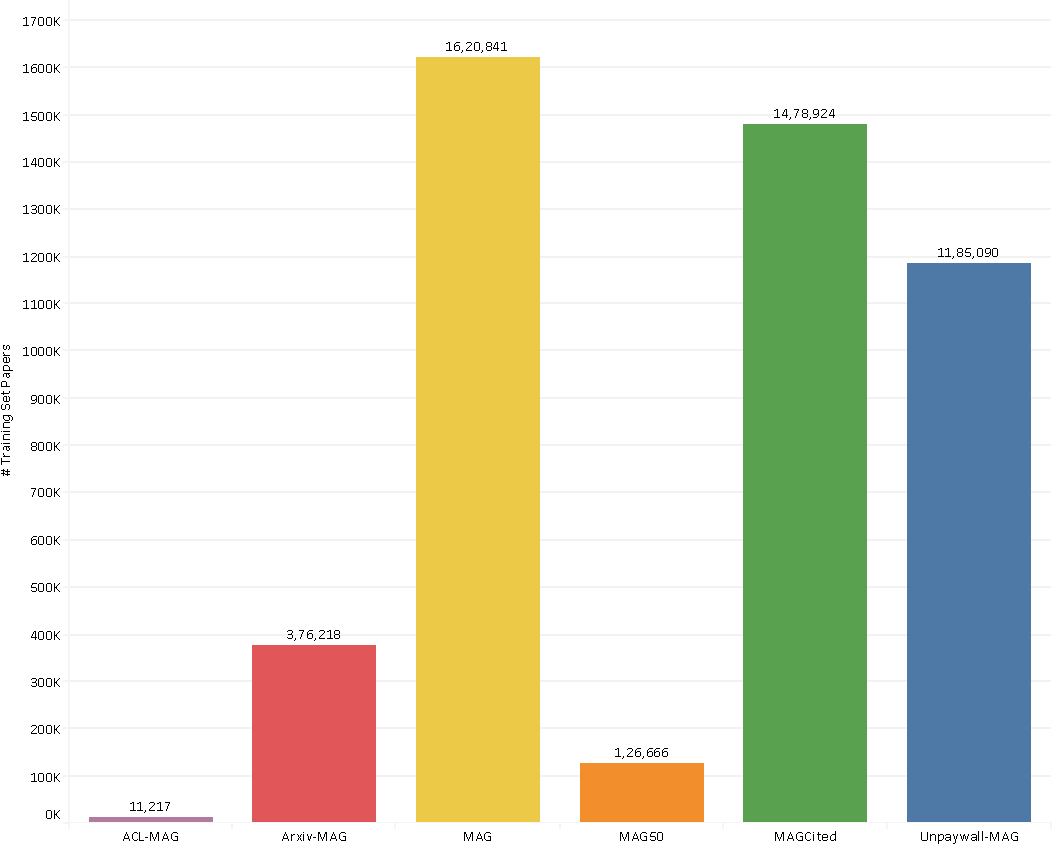
\includegraphics[width=10cm]{figures/Evaluation/trainingteststats.pdf}
    \caption{No. of training set papers per data set}
    \label{fig:trainingsetpapers}
\end{figure}
\begin{figure}
    \centering
    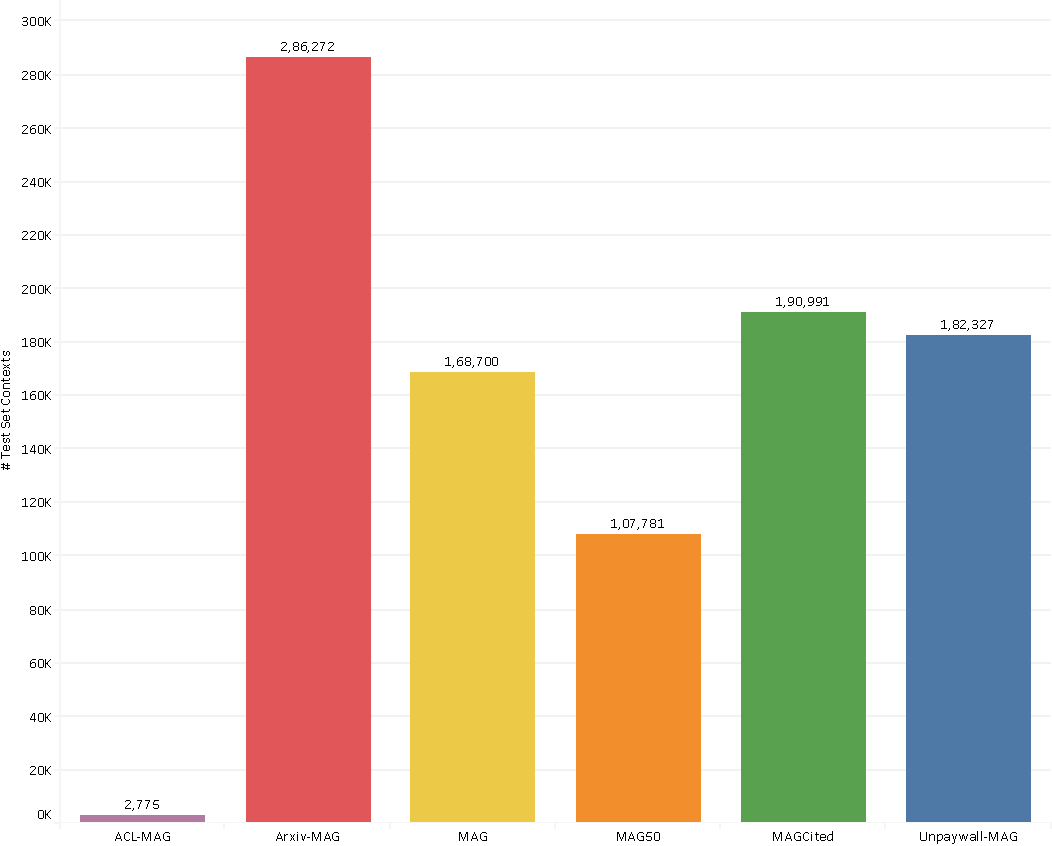
\includegraphics[width=10cm]{figures/Evaluation/testsetcontexts.pdf}
    \caption{No. of test set contexts per data set}
    \label{fig:testsetcontexts}
\end{figure}
\subsection{Offline evaluation across data sets}
Four metrics from Section 6.1 are used in the offline evaluation -- Recall, MRR, NDCG and MAP. Of these, NDCG is a useful metric only for data sets which have grading of relevant items -- where some items are 'more relevant' than others. The only two data sets which have graded relevant items are ACL-MAG and Arxiv-MAG. But none of the test set contexts for ACL-MAG actually have more than one relevant item. So the NDCG is mainly applicable for only Arxiv-MAG. However, it is reported for the other data sets as well even though we will not talk about it at all in relation to the MAG data sets where its values can be deceptive.

The Recall is probably the most important metric in citation recommendation as it gives the percentage of the ground truths which have been recommended. MAP is generally used along with Recall in evaluation of information retrieval and in citation recommendation systems, and is also reported here. It penalises false positives, while recall penalises false negatives. As a large majority of the test set contexts (across data sets) have only one relevant paper in the ground truth, the MRR is also an important metric. It describes the rank of the highest ranked paper in cases where there is more than one element in the ground truth. 

The evaluation is performed for: 
\begin{itemize}
    \item Embedding-based algorithms: Paper2Vec, Doc2Vec, hd2vOUT, hd2vINOUT (hyperdoc2vec with OUT document vectors, and both IN and OUT document vectors respectively).
    \item Information retrieval algorithm: BM25
    \item Topic Modelling algorithm: Variational Bayes LDA used as a baseline (LDA Mallet is included for ACL-MAG)
    \item Semi-genetic hybrid algorithm based on BM25 and hd2vOUT
\end{itemize}
\begin{table}[]
\centering
    \caption{Evaluation scores at k=10 for all models using the MAG data.}
    \label{tab:magevalk10}
\begin{center}
    \begin{tabular}{lllll}
    \toprule
    Model & MRR@10 & Recall@10 & MAP@10 & NDCG@10 \\
    \midrule
    hd2vOUT  & 0.0974 & 0.2149 & 0.0969 & 0.1430 \\
    BM25       & 0.1146 & 0.2098 & 0.1141 & 0.1540 \\
    hd2vINOUT & 0.0134 & 0.0194 & 0.0133 & 0.0167 \\
    Hybrid  & \textbf{0.1422} & \textbf{0.3087} & \textbf{0.1414} & \textbf{0.2051} \\
    LDA     & 0.0123 & 0.0307 & 0.0123 & 0.0192 \\
    Paper2Vec        & 0.0006 & 0.0020 & 0.0007 & 0.0011 \\
    Doc2Vec       & 0.0000008 & 0.000005 & 0.0000008 & 0.000006 \\
    \bottomrule
    \end{tabular}
\end{center}
\end{table}
\subsection{Evaluation of MAG data sets}
Figure~\ref{fig:magevaluation} shows the evaluation metrics for all the models tested using the MAG data set without any restriction on the number of citations. The evaluation results for all the models at k=10 using the MAG data set are given in Table~\ref{tab:magevalk10}.

It is clear from the graph and the table that the hybrid model has the best results using every metric. This is not a surprise as it combines the best parts of the next 2 best models, BM25 and hd2vOUT. While hd2vOUT has marginally higher recall, BM25 has slightly higher MRR and MAP. 
Unlike the other data sets we will look at shortly, hd2vINOUT performs very badly. This indicates that using the contexts and the abstract as pseudo full-text has not quite paid off in terms of the quality of IN embeddings. The much higher hd2vOUT values show that the OUT embeddings are of much better quality. The OUT embeddings correspond to the papers playing the role of a cited document, so this shows that Hyperdoc2vec is highly context-aware. 
\begin{figure}
    \centering
    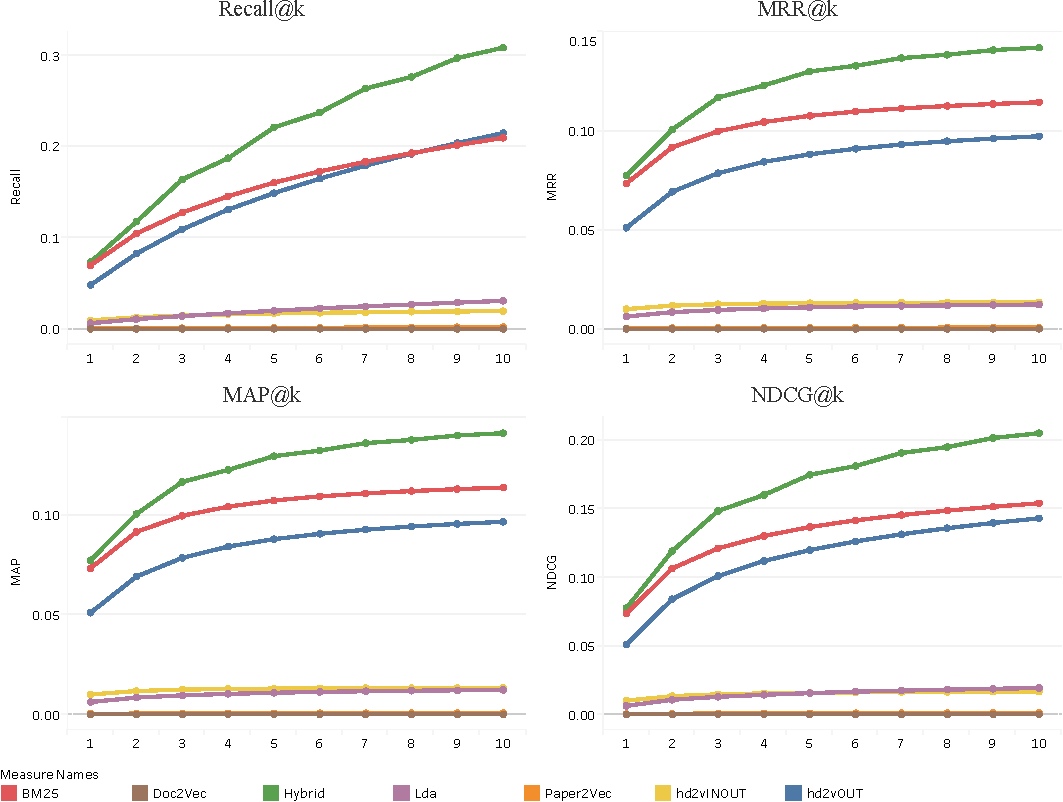
\includegraphics[keepaspectratio, width=.9\linewidth]{figures/Evaluation/MAGMetricsGraph.pdf}
    \caption{Evaluation using MAG}
    \label{fig:magevaluation}
\end{figure}

\begin{figure}
    \centering
    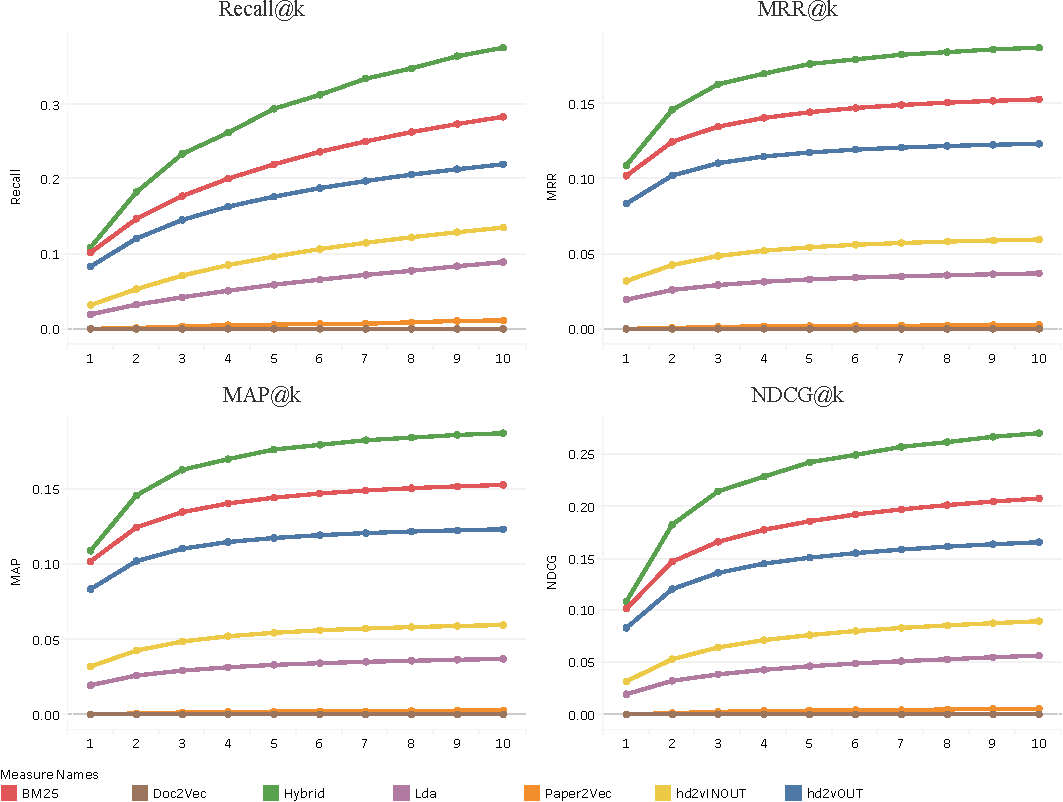
\includegraphics[keepaspectratio, width=.9\linewidth]{figures/Evaluation/MAG50MetricsGraph.pdf}
    \caption{Evaluation using MAG50: only papers with >= 50 citations in training set}
    \label{fig:mag50evaluation}
\end{figure}

The performance of LDA is below average, but it does better than hd2vINOUT for the MAG data set. Paper2Vec and Doc2Vec perform abysmally across metrics. While Paper2Vec is a lot better than Doc2Vec (the DeepWalk has clearly made a difference), it does not do a good job by any means.
\begin{table}[]
\centering
    \caption{Evaluation scores at k=10 for all models using the MAG50 data.}
    \label{tab:mag50evalk10}
\begin{center}
    \begin{tabular}{lllll}
    \toprule
    Model & MRR@10 & Recall@10 & MAP@10 & NDCG@10 \\
    \midrule
    hd2vOUT  & 0.1233 & 0.2200 & 0.1233 & 0.1660 \\
    BM25       & 0.1528 & 0.2836 & 0.1528 & 0.2082 \\
    hd2vINOUT & 0.0595 & 0.1353 & 0.1873 & 0.0898 \\
    Hybrid  & \textbf{0.1873} & \textbf{0.3760} & \textbf{0.1873} & \textbf{0.2711} \\
    LDA     & 0.0369 & 0.0892 & 0.0369 & 0.0567 \\
    Paper2Vec        & 0.0025 & 0.0113 & 0.0026 & 0.0055 \\
    \bottomrule
    \end{tabular}
\end{center}
\end{table}
Figure~\ref{fig:mag50evaluation} shows the evaluation results for all the models using the MAG50 data set -- MAG with the restriction that papers in the training set (which are to be be recommended) should have at least 50 citations. Only test set contexts with papers in the ground truth that have at least 50 citations are retained.

One would expect that MAG50 would produce better results for all the algorithms on all the metrics, and that is indeed the case at k=10 (see Table~\ref{tab:mag50evalk10}). All the metric values are significantly higher for all the data sets. This is because the data sets are of similar quality, but the number of candidates for each recommendation is much smaller for MAG50 than MAG. Consequently, it is more likely that the relevant items are near the top of the list of recommendations.  

However, the inference cannot be made that a system using MAG50 always produces better results. Less popular papers and very new papers are not recommended while using the MAG50 data set even though they may be perfectly valid recommendations. But some users might might want to be recommended only papers with a lot of citations in a running citation recommender system. So HybridCite, the final recommender system (described in Section 5.6), uses two models under the hood -- one using MAG data and the other using MAG50 data. 
\subsection{Case study using BM25 on 2 MAG data sets}
In this subsection, we perform a small case study to test the assertion made in Huang et al's two papers~\cite{HuangKCMGR12,Huang2015} that citation contexts describe the cited paper rather than the citing paper. This is done using the BM25 algorithm, which is best suited to prove this point.
\begin{figure}[h]
    \centering
    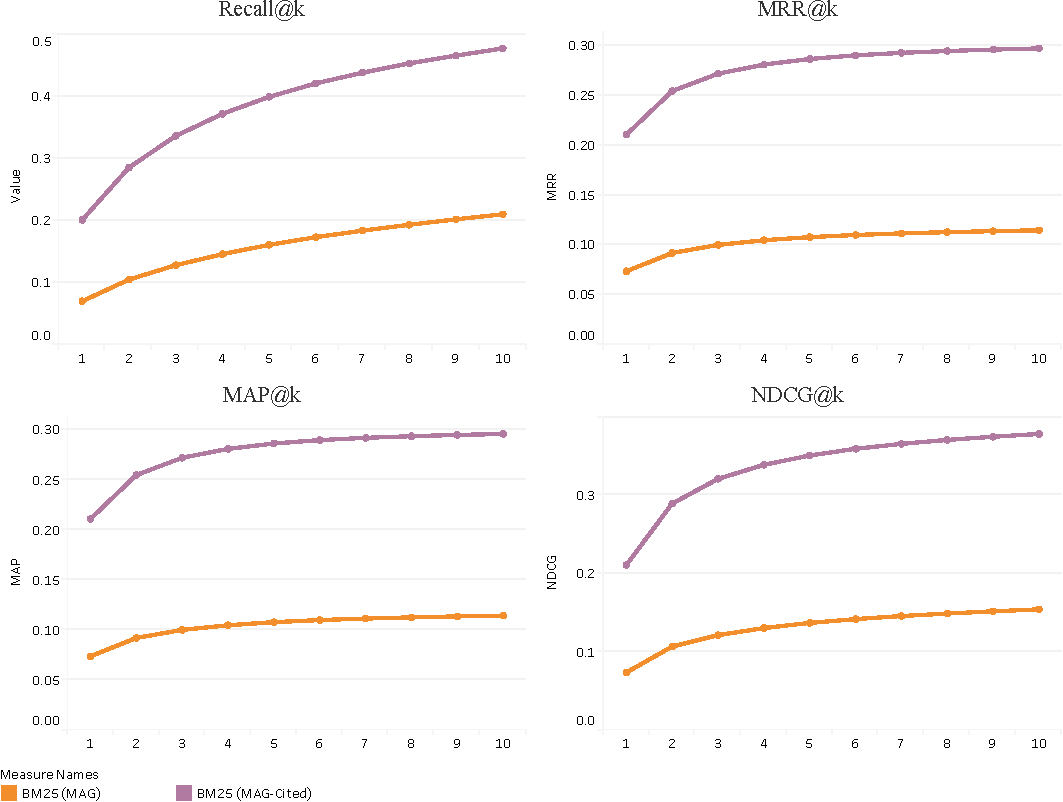
\includegraphics[keepaspectratio, width=.9\linewidth]{figures/Evaluation/MagCitedMetricGraphs.pdf}
    \caption{Comparison of BM25 Evaluation for 2 MAG data sets: MAG and MAG-Cited}
    \label{fig:magcitedevaluation}
\end{figure}
\begin{figure}
    \centering
    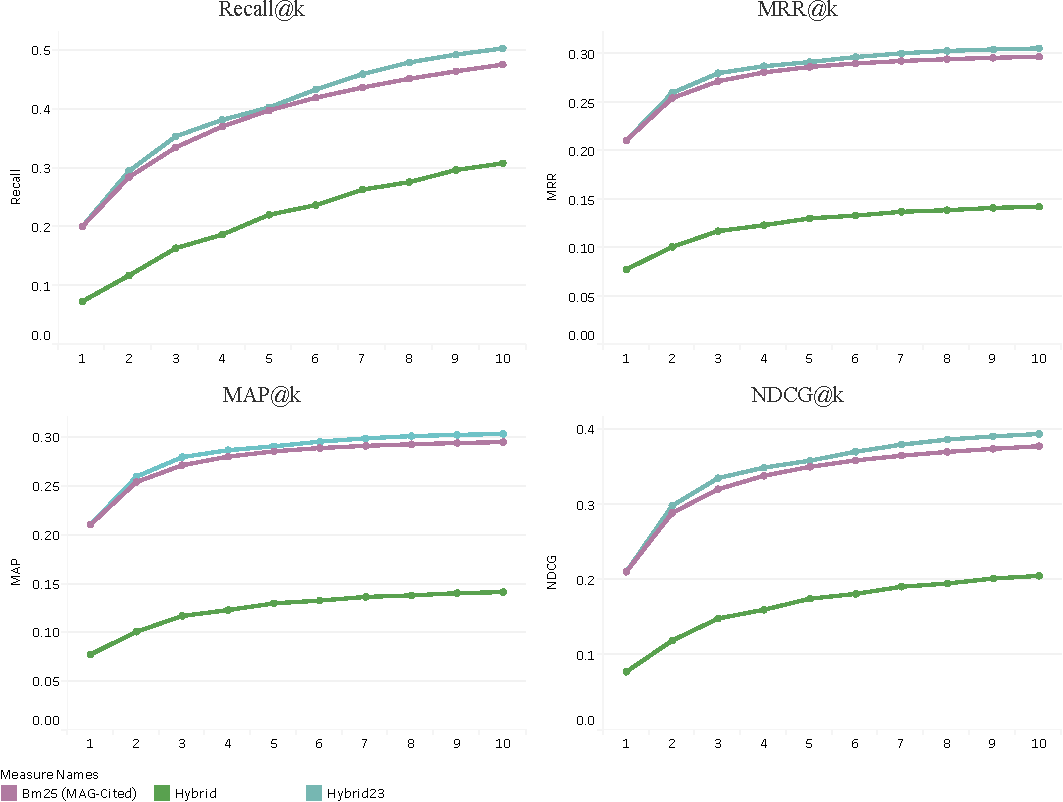
\includegraphics[keepaspectratio, width=.9\linewidth]{figures/Evaluation/MAGHybridv2metrics.pdf}
    \caption{Comparing Hybrid23 with BM25 (MAG-Cited) and the original Hybrid algorithm}
    \label{fig:maghybridevaluation}
\end{figure}
For the purpose of doing the case study, a new data set called MAG-Cited was created (the creation process is described in Section 4.2.6). The text for each paper is made up of its title, abstract and \textit{citation contexts from papers which cite it}. In other words, the content of a cited paper contains citation contexts from all its citing papers.
The text for each paper in the regular MAG data set, on the other hand, is made up of its title, abstract and citations contexts (i.e., citation contexts from its own content). 

Running the BM25 algorithm on both the data sets, we find that there is a very large difference in the evaluation results. The metrics show that using the citation contexts of a citing paper as the content of a cited paper pays off. The evaluation results are shown in Figure~\ref{fig:magcitedevaluation} and prove Huang et al's assertion pretty comprehensively. 

This result has the potential to improve recommendation results when used in a hybrid recommender system. So, an improved hybrid system (called Hybrid23) was built using two data sets and three components. The system in explained in Section 5.5.

As already explained, the Hybrid23 system retrieves recommendations from BM25 trained on the MAG data set, hd2vOUT trained on the MAG data set, and BM25 trained on the MAG-Cited data set. The goal is to get better performance than the BM25 algorithm trained on MAG-Cited, which already performs much better than the original hybrid algorithm. So in our weighted hybrid model, we use the weights (1/5, 1/5, 3/5) for our three components BM25 (MAG), hd2vOUT and BM25 (MAG-Cited). \\
The graphs in Figure~\ref{fig:maghybridevaluation} compare the original hybrid algorithm with Hybrid23 and BM25 trained on MAG-Cited. Comparing Hybrid23 and BM25 (MAG-Cited), we see that the Recall, MAP and MRR start to get higher for Hybrid23 as k becomes bigger. The recall curves, especially, start to diverge around k=5. Both algorithms are well ahead of the original hybrid algorithm on all the metrics. 

The values of the metrics at k=10 are given in Table~\ref{tab:maghybridcited}. A quick look at this table makes it clear that Hybrid23 and BM25 (MAG-Cited) have MAP and MRR values twice as large as the Hybrid algorithm at k=10. Their Recall is also substantially larger. It is also interesting to note the differences between BM25 (MAG-Cited) and Hybrid23. While there is not too much difference between their MAP and MRR values at k=10, a 2.5\% gain in Recall is very significant. In fact, the Recall@10 is more than 1/2 for Hybrid23, which indicates that a paper from the ground truth is found in the top 10 recommendations in half the test cases. 
\begin{table}[]
\centering
    \caption{Comparing evaluation scores at k=10 for BM25 (MAG-Cited), Hybrid and Hybrid23}
    \label{tab:maghybridcited}
\begin{center}
    \begin{tabular}{lllll}
    \toprule
    Model & MRR@10 & Recall@10 & MAP@10 & NDCG@10 \\
    \midrule
    Hybrid  & 0.1422 & 0.3087 & 0.1414 & 0.2051 \\
    BM25 (MAG-Cited) & 0.2970 & 0.4769 & 0.2952 & 0.3777 \\
    Hybrid23  & \textbf{0.3056} & \textbf{0.5044} & \textbf{0.3035} & \textbf{0.3940} \\
    \bottomrule
    \end{tabular}
\end{center}
\end{table}
\subsection{Evaluation of full text data sets with 'pseudo full text' from MAG}
In this part of the thesis, we will look at the evaluation results of the three data sets (Arxiv-MAG, ACL-MAG and Unpaywall-MAG) for which we have both full text as well as pseudo full-text from MAG for cited papers which don't have full text. Pseudo full-text for a paper, as already explained in Chapter 4, consists of its title, abstract and all its citation contexts from MAG. 
In this section, the evaluation results for these data sets will be compared both with those of the MAG and with each other. 
The evaluation results at k=10 for these data sets are given in Appendix~\ref{chap:fulltexteval}.

Analysing the evaluation results for Arxiv-MAG from Figure~\ref{fig:arxivmagevaluation}, we see some interesting patterns. Unlike MAG, hd2vOUT performs better than BM25 across metrics. In fact, hd2vINOUT performs almost as well as BM25. This proves an important point. Hyperdoc2Vec produces better IN embeddings (IN document vectors) when the full content is available for a large number of papers. The presence of accurate positions of citation markers in the content from Arxiv might have played a role in pushing the performance of hd2vOUT over the text-based BM25 algorithm. This is due to better quality OUT document vectors. While Arxiv-MAG also contains pseudo full-text papers, it clearly does better with IN embeddings due to the presence of many papers with full text from Arxiv. 

LDA, again, obtains mediocre results on the metrics. Paper2Vec and Doc2Vec's performance show again why they were not worth using in the hybrid algorithm. 

Comparing the concrete values of the metrics for Arxiv-MAG (see Appendix~\ref{chap:fulltexteval}) and MAG at k=10, we see that MAP and MRR for hd2vOUT are higher for Arxiv-MAG than for MAG at k=10 (across algorithms). One important consideration to take into account is that Arxiv-MAG has a higher percentage of test contexts with more than 1/2/3 papers in the ground truth (see Table~\ref{tab:groundtruthscomparison}). This improves the probability of getting some of them in the top 10 results, and therefore improves the MAP and the MRR.
\begin{table}[]
    \centering
    \begin{tabular}{ccccc}
    \toprule
    Data set & 1 ground truth paper \% & 2 ground truth papers \% & >2 ground truth papers \% \\
    \midrule
        MAG & 91.26\% (153953) & 6.04\% (10183) & 2.70\% (4564) \\
        Arxiv-MAG & 67.57\% (256037) & 16.96\% (64281) & 15.46\% (58599)\\
    \bottomrule
    \end{tabular}
    \caption{Comparison of Percentage of papers in ground truth between Arxiv-MAG and MAG (number of cases in parentheses). ACL-MAG has only one ground truth in its contexts, Unpaywall-MAG uses the same test set as MAG}
    \label{tab:groundtruthscomparison}
\end{table}
There is not much difference between the performance of BM25 on the MAG and Arxiv-MAG data sets using the MAP and MRR metrics. This is interesting as it indicates that BM25 does better on MAG. This could be because a text-based algorithm like BM25 might do better when the text content is homogeneous across papers. MAG has pseudo-full text for all papers, while Arxiv has full text for some papers and pseudo-full text for others.

The Recall is consistently higher across algorithms for MAG than Arxiv-MAG. This, again, might have a lot to do with the presence of a lot of ground truths with 4 or more papers in Arxiv-MAG (see Table~\ref{tab:groundtruthscomparison}). The Recall suffers due to this (as opposed to MAP) as a higher percentage of papers in the ground truth are missing in the top 10 results. 

The hybrid algorithm's metrics, like those of any ensemble model, can be seen as an amalgamation of the metrics of hd2vOUT and BM25.
\begin{figure}
    \centering
    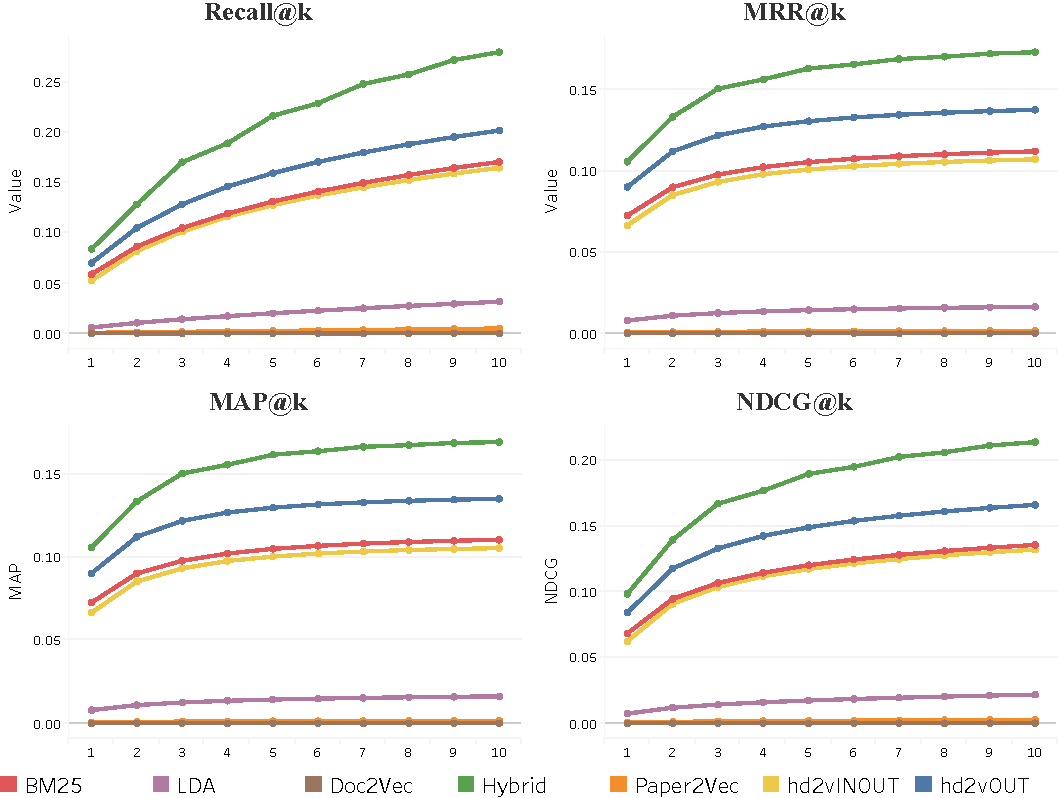
\includegraphics[keepaspectratio, width=.9\linewidth]{figures/Evaluation/ArxivMetricGraphs.pdf}
    \caption{Evaluation using Arxiv-MAG}
    \label{fig:arxivmagevaluation}
\end{figure}
\begin{figure}
    \centering
    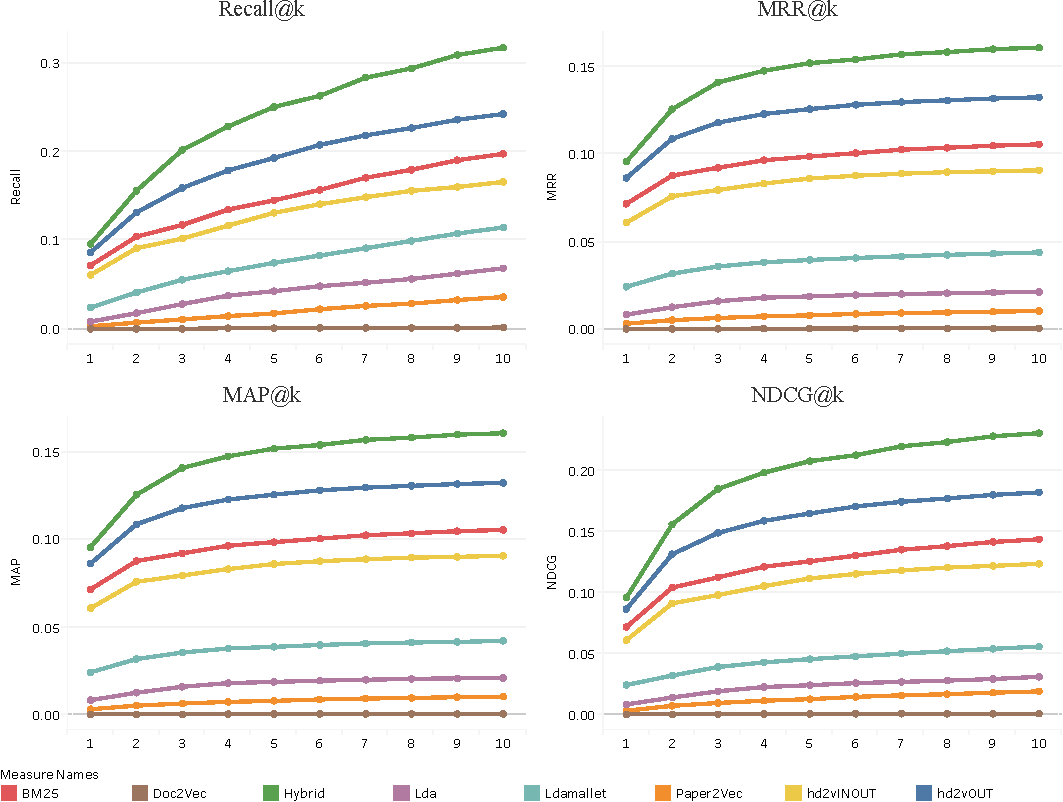
\includegraphics[keepaspectratio, width=.9\linewidth]{figures/Evaluation/ACLMetricGraphs.pdf}
    \caption{Evaluation using ACL-MAG}
    \label{fig:aclmagevaluation}
\end{figure}
Moving on to ACL-MAG, which has a very low number of test set contexts, we notice a few common patterns in Figure~\ref{fig:aclmagevaluation}. Using every metric, the performance of hd2vOUT is better than BM25, which is closely followed by hd2vINOUT. This reinforces the point made while analysing the Arxiv evaluation results that the IN document embeddings are better when some papers have full text.

Here, we also introduce a new LDA Mallet model in the results, which uses Gibbs sampling. This is said to be a better version of the Variational Bayes variant used with the other data sets, and the evaluation results bear that out. As pointed out earlier, the run time for LDA Mallet prediction is forbiddingly high. The considerable gap between LDA Mallet and the better algorithms in the graphs and the high execution time were the reasons why it wasn't used for the other data sets. 
The higher MAP and MRR when compared with MAG may simply be because of the sheer difference in size of the test sets.
\begin{figure}
    \centering
    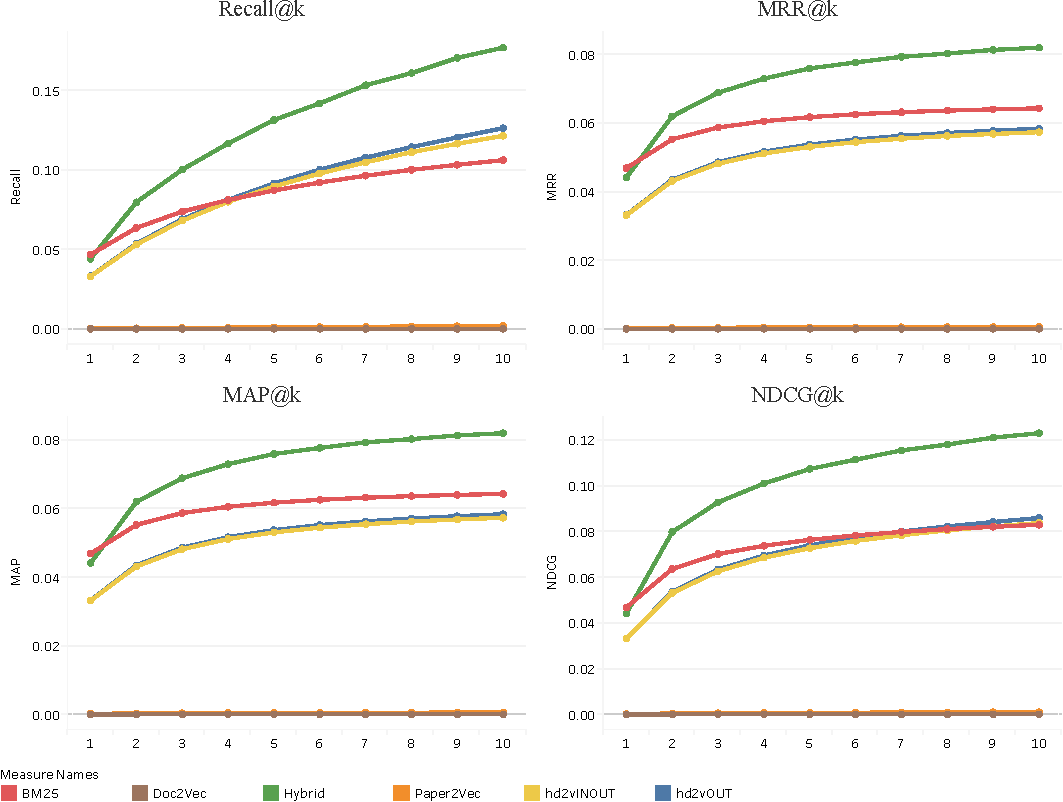
\includegraphics[keepaspectratio, width=.9\linewidth]{figures/Evaluation/UnpaywallMetricsGraph.pdf}
    \caption{Evaluation using Unpaywall-MAG}
    \label{fig:unpaywallmagevaluation}
\end{figure}
Lastly, we compare Unpaywall-MAG with Arxiv-MAG. The hd2vOUT and hd2vINOUT curves are very close to each other across metrics in the Unpaywall-MAG evaluation, but the concrete values are much lower than those for Arxiv-MAG. However, the recall rises more steeply with k for Unpaywall-MAG compared to Arxiv-MAG. The explanation for this might be that the same MAG test set is used for Unpaywall-MAG and the number of ground truths with more than one paper is not high. 

The low evaluation scores indicate that in general, the quality of embeddings for Unpaywall-MAG might be much lower than the Arxiv-MAG and MAG data sets. This is the reason all the algorithms (including BM25) do so much worse on Unpywall-MAG data than on the Arxiv-MAG and MAG data. This might be a signal that the conversion of PDF into XML using Grobid might have introduced some noise.  

At the end of the offline recommendation phase, we see a clear hierarchy in the performance of the algorithms across data sets and evaluation metrics. The hybrid algorithm performs the best and the two components of the hybrid algorithm, hd2vOUT and BM25 are the second and third best. There are some metrics and data sets for which BM25 performs better than hd2vOUT and some metrics and data sets for which it is the other way around. This is followed by hd2vINOUT and LDA. The other embedding algorithms, Paper2Vec and Doc2Vec, perform very badly. \\
As our main focus is on the MAG data sets, the online phase will use only the MAG data set, and the evaluation will be done for only the top 3 algorithms: Hybrid, BM25 and hd2vOUT.
\section{User Study and Online evaluation}
While the offline evaluation gives us an idea about how well the recommendation algorithms works, it does not paint the whole picture. Despite restricting test citation contexts from MAG to those with at least nine words (excluding stop words), it is entirely feasible that many of the contexts are too general to make any worthy recommendations. It is also possible that the citation contexts are noisy -- it might contain just formulae for example. 

This is reason enough to carry out a user study where a user manually rates the recommendations for a number of citation contexts using three algorithms: hd2vOUT, BM25 and the hybrid algorithm. It is important to note that Hybrid23 is not included in the user study. The reason for this is that we have restricted the user study to the best algorithms which work on a single data set. The user study is carried out only for the MAG data set (with no restriction on the number of citations) and is explained below.

The first step is the selection of a test set. Citation contexts are extracted from the MAG based on language and field of study. English citation contexts are chosen from the Natural Language Processing field as it closely relates to the topic of the thesis. All the citation contexts are chosen from 2018 and 2019. To make sure these contexts were seen in the offline evaluation test set, contexts which cite papers not from the training set are discarded. Duplicate contexts are grouped together. Additionally, citation contexts with 8 or fewer words (stop words not included) are discarded. 
\begin{figure}
    \centering
    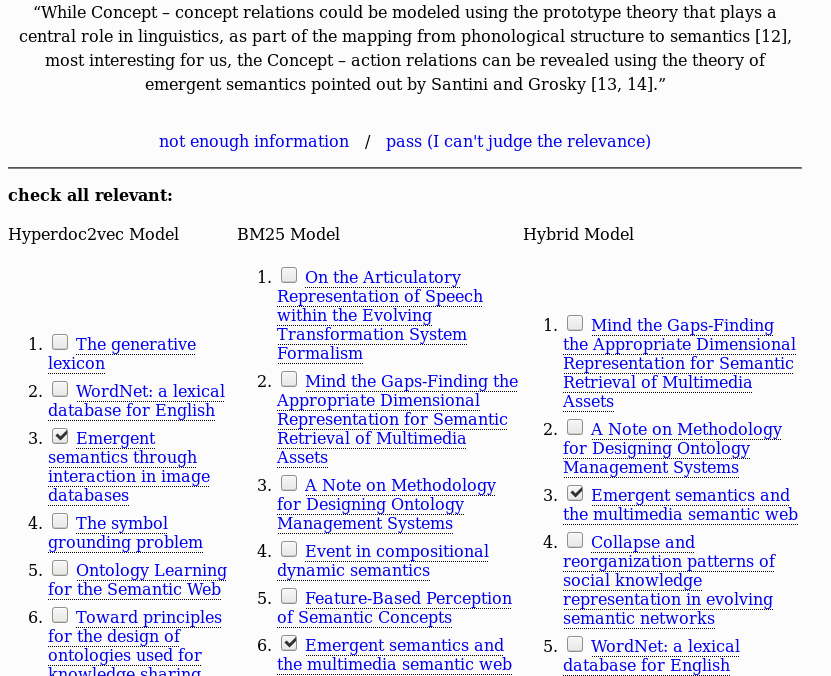
\includegraphics[keepaspectratio, width=.8\linewidth]{figures/Evaluation/userstudyinterface.PNG}
    \caption{User Study interface for example citation context}
    \label{fig:userstudyinterface}
\end{figure}
From the 8356 surviving citation contexts, random sampling is done to pick 100 citation contexts for the user study. 10 recommendations are made for each of these 100 citation contexts using each of the three chosen algorithms. The corresponding metadata -- title, abstract and the published year-- are retrieved from the MAG database. 
The recommendations, coupled with the metadata from MAG, are inserted in a JSON file. 

A web interface reads in these recommendations, and allows the user to select all the papers which are valid recommendations. The titles of the recommended papers are provided, with the corresponding abstracts in a tooltip. If the user can't understand the citation well enough to find suitable recommendations, he can select the 'pass' option. If the user believes there is not enough information in the context for it to be possible for a valid recommendation to be made, he selects the 'not enough information' option.
The user interface is shown in Figure~\ref{fig:userstudyinterface} for an example context. Here, it can be seen that one paper each is marked as valid for each of the algorithms. It is the same recommendation made by BM25 at position 6 and the hybrid algorithm at position 3. Incidentally, the ground truth for the same citation context during the offline evaluation consisted of the same papers. The hybrid algorithm misses one of them in the top 10 results. 

It is important to note that the selection of the relevant papers by the user was done based on the citation context only. So in case of contexts which are too short/general to convey the type of paper the author wanted to cite, the user had no choice but to pick recommender papers which relate to the general concept(s) in the citation context. \\
At the end of the binary rating process, 19 contexts were passed/not rated. So the total number of contexts for the online evaluation is 81.

Once the rating process for all the papers using the three models is completed, the recommendations are converted into arrays containing the positions at which the relevant papers were found. So, there are three arrays containing the positions of the relevant items for each of the three models: bm25, hd2vOUT and hybrid. These arrays are converted into binary arrays of size 10 with the positions of the relevant papers changed to ones. For example, if for a context, BM25 recommends [5,7], the corresponding binary array is [0,0,0,0,1,0,1,0,0,0].

The number of relevant papers for a test citation context is unavailable, unlike in the offline evaluation process. Instead, an approximation is made. The number of relevant results is approximated to be the sum of the results returned by hd2vOUT and BM25. The reason for this approximation is that in a vast majority of cases, the valid results picked by the user for the hybrid algorithm were from the top 10 results of hd2vOUT and BM25. The two individual models often complement each other, and pick different results. In many cases, hd2vOUT was found to recommend more general results (for example survey papers and oft-cited papers), while BM25 was found to recommend more specific results . This approximation only affects the calculation of one metric -- recall.

Three metrics are reported for the online evaluation: MAP, MRR and Recall. The NDCG is not reported because the recommendations are binary and not graded.
The calculated metrics (with recall subject to the aforementioned approximation) are shown in Table~\ref{tab:onlineevalresults}. 

\begin{table}[]
    \centering
    \begin{tabular}{cccc}
        \toprule
         Model & MAP@10 & Recall@10 & MRR@10  \\
         \midrule
         hd2vOUT & 0.314 & 0.385 & 0.315 \\
         BM25 & 0.362 & 0.541 & 0.380  \\
         Hybrid & 0.370 & 0.680 & 0.411  \\
         \bottomrule
    \end{tabular}
    \caption{Online evaluation at k=10 for 3 models using the MAG data set}
    \label{tab:onlineevalresults}
\end{table}

These results indicate that BM25 plays a dominant role in the hybrid algorithm, and outperforms hd2vOUT. However, there are a number of caveats with the online evaluation. The number of test set contexts is very small. The selection of relevant papers by the user are subjective and the citation contexts are sometimes ambiguous. The recommendations were selected only from one small field of study of computer science -- natural language processing. It isn't clear if choosing one field of study for the user study is representative of all computer science papers. 

But despite all the caveats, the user study allows us to make a number of inferences. hd2vOUT sometimes recommended some general papers relating to the concepts or claims mentioned in the citation contexts. BM25, being a text-based algorithm, recommended more specific results. As a result, their combination in the hybrid algorithm tends to combine the best of both worlds. 

Another observation was that even recommendations which are not perfectly suitable ones for the citation context might still be interesting to the end user. There are sometimes papers which touch on the topic of the citation context, or survey papers about a related research topic that might be useful. This \textit{serendipity} is a hallmark of recommender systems in general, and it could help researchers discover new topics related to their research areas.

The user study also shows that there are a number of citation contexts for which no recommendations are possible. Finally, it confirms the belief from the offline evaluation that BM25 and such text-based information retrieval algorithms work as well or better on the citation recommendations task as more complex algorithms.

Finally, the results of the user study indicate that users of the HybridCite citation recommendation system should be given an option to remove popular papers (which they are already likely to know). The hybrid algorithm often recommended such general, popular papers because hd2vOUT recommended them. So the user has been given the option of only being recommended papers with 500 or fewer citations in the HybridCite recommemder system.
    \chapter{Conclusion}\label{chap:conclusion}

In this thesis, the field of local citation recommendation was explored using the Microsoft Academic Graph data set, and a hybrid recommender system was created. Five major algorithms were investigated: 4 based on embeddings (Doc2Vec, Paper2Vec and 2 HyperDoc2Vec algorithms), 1 based on topic modelling (LDA) and 1 based on infromation retrieval (BM25). 
To this end, six data sets were created and made public. The main data source, MAG, does not provide full text. So, a data set was created wherein the title, abstract and citation contexts were combined to form what is referred to in this thesis as 'pseudo full-text'. A restricted version of the MAG data set containing only papers with 50 or more citations (MAG50) was also created. In addition to this, full text from 3 other data sources was combined with pseudo full-text from MAG, and used for evaluation.

By conducting an offline evaluation on large test sets, it was found that 2 of the embedding algorithms, Doc2Vec and Paper2Vec, do a pretty poor job at citation recommendation. LDA, while it performs marginally better, still does a poor job on all the metrics. The Hyperdoc2vec model produces two different embeddings for each paper -- IN embeddings model the paper's role as a citing paper, and OUT embeddings model the paper's role as a cited paper. Through our offline and online evaluation, we found that using only the OUT embeddings (called hd2vOUT in the thesis) for prediction produced the best scores across metrics. Using both vectors resulted in worse evaluation scores. The BM25 algorithm, which is based on text matching, compared well with most of the other algorithms.

While hd2vOUT outperformed BM25 on the evaluations using the full text-based data sets, the two algorithms were very close while evaluating on MAG, especially on the Recall metric.

By doing a user study, it was found that hd2vOUT often produces results that are more general, while BM25 produces more specific results. Thus, they complemented each other well. 

Recommendations from both algorithms were combined stochastically using a semi-genetic hybrid recommendation algorithm. This hybrid algorithm/model drastically outperformed its components on all metrics and data sets in the offline evaluation results. The user study compared the hybrid model's recommendations with those of the individual BM25 and hd2vOUT models. It was found that while there were cases where the most relevant results from the individual algorithms were missing from the hybrid model's recommendations, this did not happen often. The hybrid model's recommendations generally tended to produce more relevant results than either of the individual models.

In addition, it was found that the hybrid model satisfied the serendipity requirement of recommender systems, where papers were recmmended which might be interesting to the user, even if they are not the papers they would want to recommend.

By performing a case study, it was demonstrated that using citing paper's citation contexts as part of a cited paper's content improved the performance of BM25 many times over. A separate data set called MAG-Cited was created for this purpose. Each paper's content in this data set was its title, abstract and citation contexts from papers which cite it. The excellent performance of BM25 on MAG-Cited suggested the possibility of creating a second hybrid model, based on two data sets and three components. This hybrid model, called Hybrid23, performed much better than the original hybrid model (whose two components are the first two components of Hybrid23) and marginally better than the its third component, BM25 based on MAG-Cited.
The Hybrid23 model was finally plugged into a running recommender system, where the user can enter his/her citation context and get recommendations. A second hybrid model based on the MAG50 data set was also used under the hood of the recommender system to give the user another option while getting recommendations.

Overall, it was clear that citation recommendation is a far from simple task, as borne out in both the offline and online evaluation results. The hybrid algorithms performed much better than their individual components, but they can be improved by improving their components. Using a hybrid algorithm based on two distinct MAG data sets created a much better citation recommendation system as the data was more representative.
    \chapter{Future work}

The thesis presented a working citation recommendation system, but there are multiple areas in which further research can be carried out. These areas will be touched upon in this chapter. 

Of course, a hybrid or ensemble algorithm is only as good as its components. While BM25 and hd2vOUT are used for this hybrid model, more complex deep learning-based algorithms could be used to further improve the quality of citation recommendations. 

Another set of algorithms which could be used in the hybrid model could be semantic algorithms which work based on specific components in a citation context. It can help to identify if a concept has been defined in the citation context, or if a certain claim has been made. We can then use a separate algorithm for recommending citations for a concept and for a claim. This would then need the creation a 'switching' hybrid recommender system as described in \cite{Burke2002}. 

A classifier to identify citation context types was built while doing work on the thesis, but it was trained on a very small data set and it was not clear if it would generalise well. So it wasn't used. This classifier, if it works satisfactorily, should be able to identify concepts and claims as well as 'incomplete' contexts -- contexts for which no valid recommendation can be made. These contexts can then automatically be discarded during the training phase. Better quality training data leads to better results. 

The case study in Section 6.2.4 showed that the BM25 algorithm worked much better when a cited paper's content was made up of citation contexts from papers which cite it. This is in line with observations made in \cite{HuangKCMGR12}. 
Hybrid23, the hybrid recommender system built based on this case study, performed better than all its components. The weights in the weighted hybridisation algorithm can be tuned further, which might improve the results. 
This case study can be tested futher by creating more data sets other than MAG, including some based on full-text data sets. This will need extraction of citation contexts from citing papers, and inserting them in the cited papers. 

There are a number of other possibilities for future work relating to this thesis. It would be an interesting exercise to compare citation recommendation across different disciplines. This thesis uses computer science, but it might be the case that a discipline in the humanities may work better with citation recommendation.
This could also then lead to further research on obtaining cross-domain recommendations. In a world where the lines between disciplines are increasingly being blurred, this might be very useful as researchers would be introduced to areas of study he/she hadn't thought about. 

Another road we could travel down would be to attempt to tackle the problem of cross-language recommendation -- recommending English citations for French and German papers for example. Cross-language recommendation in English/Chinese has been explored by many authors in existing research (\cite{TangWZ14,JiangLL18, JiangYGLL18}). The ability to recommend papers in a different language would add an additional dimension to the citation recommendation system. Embedding-based models in theory should work well with cross-language recommendation as embeddings are not language-specific by nature. Information retrieval approaches will not work well, so an alternative will have to be found in this case. 

All in all, there is plenty of scope for future work on this topic.

    % bibliography is not in the table of contents per default, add it manually
    % enable the \renewcommand for german header
    % \renewcommand{\bibname}{Literaturverzeichnis}
    \addcontentsline{toc}{chapter}{Bibliography}

    \bibliographystyle{ieeetr}
    \bibliography{bib/paper}

    \newpage  % makes Appendices page start at A1 instead of A3
    \pagenumbering{arabic}  % resets `page` counter to 1
    \renewcommand*{\thepage}{A\arabic{page}}
    \begin{appendices}
    \chapter{Offline evaluation data filter criteria}\label{chap:offlineevalfilter}

Table~\ref{tab:datasetfilter} details the filter criteria used while choosing the final list of papers for each training set. The MAG data set is based on a snapshot from February 2019 provided by Microsoft. During preparation of the Unpaywall-MAG data set, a JSONlines file from September 2018 is was used. The Arxiv portion of the Arxiv-MAG data set is from the data set described in Saier et al.~\cite{SaierF19}. An earlier version of this data set, which contains papers up until 2017, was used in the Arxiv-MAG data preparation phase. The ACL-ARC data in the ACL-MAG data set uses the same data used in Färber et al.~\cite{Faerber2018b} \footnote{This data is available at \url{http://citation-recommendation.org/publications/#To_Cite_or_Not_to_Cite}}.

\begin{table}
\centering
    \caption{Filter criteria for offline evaluation data.}
    \label{tab:datasetfilter}
\begin{center}
    \begin{tabular}{lp{11.5cm}}
    \toprule
    Data set & Filter criteria\\
    \midrule
    MAG & Training set papers were chosen from the field of Computer Science. Only English papers were chosen. The abstract in the MAG database was non-null for the chosen papers. The papers in the training set are from 1800 to 2017 (the test set used contexts from 2018 and 2019).\\
    \midrule
    MAG50 & Training set papers were chosen from the field of Computer Science. Only English papers were chosen. The abstract in the MAG database was non-null for the chosen papers. The papers in the training set are from 1800 to 2017 and should have been cited at least 50 times. The test set used contexts from 2018 and 2019. \\
    \midrule
    Unpaywall-MAG & Training set papers were chosen from the field of computer science. Only English papers were chosen. The abstract in the MAG database was non-null for the chosen papers. The papers in the training set are from 1800 to 2017. Of these papers, the final list of chosen papers were those which could be (i) downloaded using the links provided by Unpaywall, (ii) converted into full text using Grobid~\cite{GROBID}. The additional MAG papers fetched are those cited by the Arxiv papers which are in the MAG data set as well as those cited by \textit{these MAG papers}. The test set contained MAG citation contexts from 2018 and 2019. \\
    \midrule
    Arxiv-MAG & Training set papers were chosen from the field of computer science in the Arxiv data set such that they have at least 5 citing documents within the data set. The papers are from 1991-2016. The additional MAG papers fetched are those cited by the Arxiv papers which are in the MAG data set as well as those cited by \textit{these MAG papers}. The test set used Arxiv citation contexts from 2017.\\
    \midrule
    ACL-MAG & Training set papers chosen from the ACL-ARC data set should have been mapped to a DBLP ID. The papers are from the years 1965-2005. The additional MAG papers fetched are those cited by the ACL-ARC papers which are in the MAG data set as well as those cited by \textit{these MAG papers}. The test set contained ACL-ARC citation contexts from 2006.\\
    \bottomrule
    \end{tabular}
\end{center}
\end{table}

\chapter{Preprocessing}\label{chap:preprocessing}

Preprocessing is an extremely important step while using embedding algorithms like Hyperdoc2vec. The common preprocessing steps used for Hyperdoc2vec and Paper2Vec before both training and prediction are:

1. Expand contractions: In this step, "isn't" is expanded to is not, "aren't" is expanded to are not, and so on. The contractions are expanded using the 'contractions' package in Python.

2. Remove punctuation and special characters (this is also important for the BM25 indexing and prediction).

3. Remove additional white spaces

4. Remove stop words: algorithms like Doc2Vec, Word2Vec, and HyperDoc2vec work on the principle that a word is described by the 'company it keeps', i.e., the words it commonly co-occurs with. 
So the stop words removed play an important role in deciding the company each word keeps.
In this thesis, we remove stop words very aggressively. The stop word list is taken from \cite{StoneDK11} and is given in its entirety below.

all, six, just, less, being, indeed, over, move, anyway, four, not, own, through, using, fifty, where, mill, only, find, before, one, whose, system, how, somewhere, much, thick, show, had, enough, should, to, must, whom, seeming, yourselves, under, ours, two, has, might, thereafter, latterly, do, them, his, around, than, get, very, de, none, cannot, every, un, they, front, during, thus, now, him, nor, name, regarding, several, hereafter, did, always, who, didn, whither, this, someone, either, each, become, thereupon, sometime, side, towards, therein, twelve, because, often, ten, our, doing, km, eg, some, back, used, up, go, namely, computer, are, further, beyond, ourselves, yet, out, even, will, what, still, for, bottom, mine, since, please, forty, per, its, everything, behind, does, various, above, between, it, neither, seemed, ever, across, she, somehow, be, we, full, never, sixty, however, here, otherwise, were, whereupon, nowhere, although, found, alone, re, along, quite, fifteen, by, both, about, last, would, anything, via, many, could, thence, put, against, keep, etc, amount, became, ltd, hence, onto, or, con, among, already, co, afterwards, formerly, within, seems, into, others, while, whatever, except, down, hers, everyone, done, least, another, whoever, moreover, couldnt, throughout, anyhow, yourself, three, from, her, few, together, top, there, due, been, next, anyone, eleven, cry, call, therefore, interest, then, thru, themselves, hundred, really, sincere, empty, more, himself, elsewhere, mostly, on, fire, am, becoming, hereby, amongst, else, part, everywhere, too, kg, herself, former, those, he, me, myself, made, twenty, these, was, bill, cant, us, until, besides, nevertheless, below, anywhere, nine, can, whether, of, your, toward, my, say, something, and, whereafter, whenever, give, almost, wherever, is, describe, beforehand, herein, doesn, an, as, itself, at, have, in, seem, whence, ie, any, fill, again, hasnt, inc, thereby, thin, no, perhaps, latter, meanwhile, when, detail, same, wherein, beside, also, that, other, take, which, becomes, you, if, nobody, unless, whereas, see, though, may, after, upon, most, hereupon, eight, but, serious, nothing, such, why, off, a, don, whereby, third, i, whole, noone, sometimes, well, amoungst, yours, their, rather, without, so, five, the, first, with, make, once


Note that LDA requires further preprocessing (described in chapter 5): creation of bi-grams and stemming using a Snowball stemmer.

\chapter{Evaluation on Arxiv-MAG, Unpaywall-MAG, ACL-MAG at k=10}\label{chap:fulltexteval}
This appendix contains the evaluation results at k=10 for all the algorithms on the three data sets which are made up of full text as well as pseudo full-text from MAG: Arxiv-MAG, Unpaywall-MAG and ACL-MAG.
\begin{table}[h]
\centering
    \caption{Evaluation scores at k=10 for all models using the Arxiv-MAG data.}
    \label{tab:mag50evalk10}
\begin{center}
    \begin{tabular}{lllll}
    \toprule
    Model & MRR@10 & Recall@10 & MAP@10 & NDCG@10 \\
    \midrule
    hd2vOUT  & 0.1379 & 0.2021 & 0.1351 & 0.1660 \\
    BM25       & 0.1123 & 0.1709 & 0.1104 & 0.1357 \\
    hd2vINOUT & 0.1073 & 0.1650 & 0.1054 & 0.1666 \\
    Hybrid  & \textbf{0.1734} & \textbf{0.2801} & \textbf{0.1692} & \textbf{0.2139} \\
    LDA     & 0.0164 & 0.0316 & 0.0162 & 0.0218 \\
    Paper2Vec        & 0.0015 & 0.0049 & 0.0015 & 0.0026 \\
    Doc2Vec       & 0.000008 & 0.000016 & 0.000008 & 0.000016 \\
    \bottomrule
    \end{tabular}
\end{center}
\end{table}
\begin{table}[]
\centering
    \caption{Evaluation scores at k=10 for all models using the Unpaywall-MAG data.}
    \label{tab:mag50evalk10}
\begin{center}
    \begin{tabular}{lllll}
    \toprule
    Model & MRR@10 & Recall@10 & MAP@10 & NDCG@10 \\
    \midrule
    hd2vOUT  & 0.0584 & 0.1267 & 0.0584 & 0.0860 \\
    BM25       & 0.0644 & 0.1065 & 0.0644 & 0.0831 \\
    hd2vINOUT & 0.0574 & 0.1218 & 0.0574 & 0.0838 \\
    Hybrid  & \textbf{0.0820} & \textbf{0.1775} & \textbf{0.0820} & \textbf{0.1232} \\
    Paper2Vec  & 0.0006 & 0.0018 & 0.0006 & 0.0010 \\
    Doc2Vec       & 0.000012 & 0.000014 & 0.000012 & 0.000014 \\
    \bottomrule
    \end{tabular}
\end{center}
\end{table}
\begin{table}[]
\centering
    \caption{Evaluation scores at k=10 for all models using the ACL-MAG data.}
    \label{tab:mag50evalk10}
\begin{center}
    \begin{tabular}{lllll}
    \toprule
    Model & MRR@10 & Recall@10 & MAP@10 & NDCG@10 \\
    \midrule
    hd2vOUT  & 0.1328 & 0.2429 & 0.1328 & 0.1822 \\
    BM25       & 0.1058 & 0.1978 & 0.1058 & 0.1438 \\
    hd2vINOUT & 0.0909 & 0.1661 & 0.0909 & 0.1237 \\
    Hybrid  & \textbf{0.1612} & \textbf{0.3178} & \textbf{0.1612} & \textbf{0.2309} \\
    LDA     & 0.0212 & 0.0684 & 0.0209 & 0.0309 \\
    LDAMallet       & 0.0438 & 0.1146 & 0.0422 & 0.0557 \\
    Paper2Vec        & 0.0102 & 0.0360 & 0.0102 & 0.0188 \\
    Doc2Vec       & 0.0003 & 0.0015 & 0.0003 & 0.0006 \\
    \bottomrule
    \end{tabular}
\end{center}
\end{table}

    \end{appendices}

    \newpage
    \thispagestyle{empty}
    \mbox{}


\end{document}
